%%%%%%%%%%%%%%%%%%%%%%%%%%%%%%%%%%%%%%%%%%%%%%%%%%%%%%%%%%%%%%%%%%%%%%%%%%%%%
%                                                                           %
%          LaTeX File for Doctor (Master) Thesis of ECNU                    %
%            华东师范大学博士(硕士)论文模板 ____lizb                        %
%                                                                           %
%%%%%%%%%%%%%%%%%%%%%%%%%%%%%%%%%%%%%%%%%%%%%%%%%%%%%%%%%%%%%%%%%%%%%%%%%%%%%

\documentclass[12pt,openany,a4paper,fancyhdr,oneside]{ctexbook}
%\documentclass[12pt,openright,a4paper,fancyhdr,twoside]{ctexbook}
%draft 选项可以使插入的图形只显示外框,以加快预览速度。
%\documentclass[11pt,a4paper,openany,draft]{book}

\usepackage{multirow}
\usepackage{listings}
\usepackage{xcolor}

\usepackage[CJKbookmarks,linkcolor=black,citecolor=black]{hyperref}
\usepackage{shortvrb,indentfirst,ulem,makeidx}
\usepackage{fancyhdr}
\usepackage{graphicx}
\usepackage{indentfirst,latexsym,amsthm,colortbl,subfigure,clrscode}
\usepackage{algorithm}
\usepackage{algorithmic}
\usepackage{bm}                     % 处理数学公式中的黑斜体的宏包
\usepackage{amsmath}                % AMSLaTeX宏包 用来排出更加漂亮的公式
\usepackage{amssymb}                % AMSLaTeX宏包 用来排出更加漂亮的公式
\usepackage{mathrsfs}
\usepackage[subnum]{cases}
\usepackage[numbers,sort&compress]{natbib}
%\usepackage[super,square,numbers,sort&compress]{natbib}
\usepackage{hypernat}
\usepackage{geometry}

\usepackage{times}
\usepackage{fontspec}
\usepackage{libertine}

\usepackage{caption}
\usepackage{titletoc}


\makeindex
\pagestyle{fancy}

\fancyhead[RO,LE]{\bfseries 华东师范大学研究生硕士学位论文}
\fancyhead[LO]{\small \leftmark} \fancyhead[RE]{\small \leftmark}

\renewcommand{\headrulewidth}{0.4pt}
\fancyfoot[CO,CE]{\thepage}

\renewcommand{\algorithmicrequire}{\textbf{Input:}}
\renewcommand{\algorithmicensure}{\textbf{Output:}}
\renewcommand{\algorithmiccomment}[1]{// #1}


%                    根据自己正文需要做的一些定义                 %
%==================================================================
\def\diag{{\rm diag}}
\def\rank{{\rm rank}}
\def\RR{{\cal R}}
\def\NN{{\cal N}}
\def\R{{\mathbb R}}
\def\C{{\mathbb C}}
\let\dis=\displaystyle

\def\p{\partial}
\def\f{\frac}
\def\mr{\mathrm}
\def\mb{\mathbf}
\def\mc{\mathcal}
\def\b{\begin}
\def\e{\end}

\newtheorem{thm1}{Theorem}[part]
\newtheorem{thm2}{Theorem}[section]
\newtheorem{thm3}{Theorem}[subsection]
\newtheorem{them}[thm2]{定理}
\newtheorem{theorem}[thm2]{定理}
\newtheorem{defn}[thm2]{定义}
\newtheorem{define}[thm2]{定义}
\newtheorem{ex}[thm2]{例}
\newtheorem{exs}[thm2]{例}
\newtheorem{example}[thm2]{例}
\newtheorem{prop}[thm2]{命题}
\newtheorem{lemma}[thm2]{引理}
\newtheorem{cor}[thm2]{推论}
\newtheorem{remark}[thm2]{注释}
\newtheorem{notation}[thm2]{记号}
\newtheorem{abbre}[thm2]{缩写}
% \newtheorem{algorithm}[thm2]{算法}
\newtheorem{problem}[thm2]{问题}

\newcommand{\tabincell}[2]{\begin{tabular}{@{}#1@{}}#2\end{tabular}}

\newcommand{\yihao}{\fontsize{26pt}{36pt}\selectfont}           % 一号, 1.4 倍行距
\newcommand{\erhao}{\fontsize{22pt}{28pt}\selectfont}          % 二号, 1.25倍行距
\newcommand{\xiaoer}{\fontsize{18pt}{18pt}\selectfont}          % 小二, 单倍行距
\newcommand{\sanhao}{\fontsize{16pt}{24pt}\selectfont}        % 三号, 1.5倍行距
\newcommand{\xiaosan}{\fontsize{15pt}{22pt}\selectfont}        % 小三, 1.5倍行距
\newcommand{\sihao}{\fontsize{14pt}{21pt}\selectfont}            % 四号, 1.5 倍行距
\newcommand{\banxiaosi}{\fontsize{13pt}{19.5pt}\selectfont}    % 半小四, 1.5倍行距
\newcommand{\xiaosi}{\fontsize{12pt}{18pt}\selectfont}            % 小四, 1.5倍行距
\newcommand{\dawuhao}{\fontsize{11pt}{11pt}\selectfont}       % 大五号, 单倍行距
\newcommand{\wuhao}{\fontsize{10.5pt}{15.75pt}\selectfont}    % 五号, 单倍行距



\lstset
{
	basicstyle=\ttfamily,
	% numbers=left,
	% numberstyle=\tiny,
	keywordstyle=\color[RGB]{0, 0, 255},
	commentstyle=\color[RGB]{0, 128, 0},
	frame=shadowbox,
	rulesepcolor=\color{red!20!green!20!blue!20},
	showspaces=false,
	showstringspaces=false,
	extendedchars=false,
	showtabs=false,
	tabsize=4,
	xleftmargin=0.5em,
	xrightmargin=0.5em,
	% aboveskip=1em,
	escapeinside=``
}


%============================ 可以自定义文字块 ================================%

\newcommand{\aaa}{这是我给你们的一个示例}
\newcommand{\bbb}{\aaa \aaa \aaa}
\newcommand{\ccc}{\bbb \bbb \bbb \bbb \bbb

\bbb \bbb \bbb \bbb \bbb }
\newcommand{\abc}{abcdefg1234567890}
\newcommand{\upabc}{ABCDEFGHIJK}
%%% ----------------------------------------------------------------------



%============================= 版芯控制 ================================%
\setlength{\oddsidemargin}{0.57cm}
\setlength{\evensidemargin}{\oddsidemargin}
\voffset-6mm \textwidth=150mm \textheight=230mm \headwidth=150mm
%\rightmargin=35mm
%                                                                       %


%============================= 页面设置 ================================%
%-------------------- 定义页眉和页脚 使用fancyhdr 宏包 -----------------%
% 定义页眉与正文间双隔线
\newcommand{\makeheadrule}{%
\makebox[0pt][l]{\rule[.7\baselineskip]{\headwidth}{0.4pt}}%
\rule[0.85\baselineskip]{\headwidth}{0.4pt} \vskip-.8\baselineskip}
\makeatletter
\renewcommand{\headrule}{%
{\if@fancyplain\let\headrulewidth\plainheadrulewidth\fi
\makeheadrule}} \makeatother

\newcommand{\adots}{\mathinner{\mkern 2mu%
\raisebox{0.1em}{.}\mkern 2mu\raisebox{0.4em}{.}%
\mkern2mu\raisebox{0.7em}{.}\mkern 1mu}}

%\setmainfont{Times New Roman}
\dottedcontents{chapter}[1.5cm]{\xiaosi\heiti}{3.8em}{9.5pt}
\dottedcontents{section}[1.5cm]{\xiaosi\heiti}{2.8em}{9.5pt}


%=============================== 正文部分 ================================%
\pagestyle{empty}

\noindent{{\zihao{4} {\large 2018} 届研究生硕士学位论文}}
\hskip 4.75cm {{\zihao{4} ~~学校代号: {\large 10269}}}\\
\hspace*{\fill} {{\zihao{4} 学号: {\large 51151500019}}}

\vskip 2cm

\begin{center}
\scalebox{1.0}{
\includegraphics[width=15cm]{fig/ecnu.eps}}
\end{center}

\vskip 3cm

\begin{center}
{\zihao{2}\bf 基于协同仿真和统计模型检测的信息物理融合系统验证分析方法}
\end{center}

\vskip 3cm {\Large
\begin{center}
\begin{tabular}{l}
院\qquad\ \ \ 系:\\
专~业~名~称:\\
研~究~方~向:\\
指~导~教~师:\\
硕士研究生:
\end{tabular}
\begin{tabular}c
~~计算机科学与软件工程学院 \\
\hline  软件工程 \\
\hline  可信软件  \\
\hline ~~杜德慧\  副教授  \\
\hline ~~姜\ 凯强\   \\
\hline
\end{tabular}
\end{center}}

\vskip 30mm

\begin{center}
{\Large 2018年5月}
\end{center}

\newpage

\pagestyle{empty}

\noindent{\large 2016 MASTER’S  DISSERTATION}
\hskip 1.4cm {\large School Code: 10269}\\
\hspace*{\fill} {\large Student Number: 51131500003}

\vskip 2cm

\begin{center}
{\Huge $\mathbb{EAST}\,\mathbb{CHINA}\,\mathbb{NORMAL}\,
\mathbb{UNIVERSITY}$}
\end{center}

\vskip 3cm

\begin{center}
{\huge \bf \scshape Statistical Model Checking Based on Abstraction and Learning}
\end{center}

\vskip 2cm {\large
\begin{center}
\begin{tabular}{l}
Department:\\
			\\
Major:\\
Research Direction:\\
Supervisor:\\
Candidate:
\end{tabular}
\begin{tabular}c
~~~School of Computer Science  \\
\hline ~~and Software Engineering  \\
\hline ~~~Software Engineering  \\
\hline ~~~Trustworthy Software  \\
\hline ~~~Associate Professor ~Dehui Du~  \\
\hline ~~~Bei~Cheng  \\
\hline
\end{tabular}
\end{center}}

\vskip 30mm

\begin{center}
{\Large May, 2016}
\end{center}

\newpage
\pagestyle{empty}
\centerline{\bf\Large 华东师范大学学位论文原创性声明}

\vskip 1cm

\normalsize \indent
郑重声明:本人呈交的学位论文《基于抽象和学习的统计模型检测研究》,是在华东师范大学攻读硕士/博士(请勾选)学位期间,在导师的指导下进行的研究工作及取得的研究成果。除文中已经注明引用的内容外,本论文不包含其他个人已经发表或撰写过的研究成果。对本文的研究做出重要贡献的个人和集体,均已在文中作了明确说明并表示谢意。
$$\\  $$

\qquad\qquad{作者签名}:$\underline{\qquad\qquad\qquad }$
\qquad \qquad\qquad \mbox {日期}:\qquad 年 \qquad  月 \qquad  日


\vskip 1cm

\centerline{\bf\Large 华东师范大学学位论文著作权使用声明}

\vskip 1cm

《基于抽象和学习的统计模型检测研究》系本人在华东师范大学攻读学位期间在导师指导下完成的硕士/博士(请勾选)学位论文,本论文的研究成果归华东师范大学所有。本人同意华东师范大学根据相关规定保留和使用此学位论文,并向主管部门和相关机构如国家图书馆、中信所和“知网”送交学位论文的印刷版和电子版;允许学位论文进入华东师范大学图书馆及数据库被查阅、借阅;同意学校将学位论文加入全国博士、硕士学位论文共建单位数据库进行检索,将学位论文的标题和摘要汇编出版,采用影印、缩印或者其它方式合理复制学位论文。

本学位论文属于(请勾选)

(  )1.经华东师范大学相关部门审查核定的“内部”或“涉密”学位论文*,
于     年    月    日解密,解密后适用上述授权。

(  )2.不保密,适用上述授权。
$$\\ $$
\qquad\qquad \mbox{导师签名}:$\underline{\qquad\qquad\qquad\qquad}$
\qquad\qquad \mbox {本人签名}:$\underline{\qquad\qquad\qquad\qquad }$

\vskip 1cm

$\rightline{ \qquad 年 \qquad  月 \qquad  日 \qquad\qquad}$

\vskip 1cm

* “涉密”学位论文应是已经华东师范大学学位评定委员会办公室或保密委员会审定过的学位论文(需附获批的《华东师范大学研究生申请学位论文“涉密”审批表》方为有效),未经上述部门审定的学位论文均为公开学位论文。此声明栏不填写的,默认为公开学位论文,均适用上述授权)。

\newpage
\pagestyle{empty}
$$\\ \\ \\ $$

\centerline{\bf\Large $\underline{\mbox{\kaishu {程贝}}}\,\,
	$硕士学位论文答辩委员会成员名单}

\vskip 10mm

\begin{center}
	{\large
		\begin{tabular}{| p{25mm}| p{30mm}| p{48mm}| p{25mm}|}\hline
			\vfill\hfill{\heiti 姓名}\hspace*{\fill} &\vfill\hfill{\heiti 职称}\hspace*{\fill} &
			\vfill\hfill{\heiti 单位}\hspace*{\fill} &\vfill\hfill {\heiti 备注} \hspace*{\fill} \\[6pt]\hline
			\vfill\hfill{\kaishu 缪淮扣}\hspace*{\fill} &\vfill\hfill{\kaishu 教授}\hspace*{\fill} &\vfill\hfill{\kaishu 上海大学}\hspace*{\fill} & \vfill\hfill {\kaishu 主席}\hspace*{\fill} \\[6pt]\hline
			\vfill\hfill{\kaishu 胡豪东}\hspace*{\fill} &\vfill\hfill{\kaishu 高级工程师}\hspace*{\fill} &\vfill\hfill{\kaishu \tabincell{c}{中航工业航空动力\\控制系统研究所} }\hspace*{\fill} & \vfill{\heiti }\\[20pt]\hline
			\vfill\hfill{\kaishu 陈铭松}\hspace*{\fill} &\vfill\hfill{\kaishu 教授}\hspace*{\fill} &\vfill\hfill{\kaishu 华东师范大学}\hspace*{\fill} & \vfill{\heiti }\\[20pt]\hline
			\vfill\hfill{\kaishu ~~~}\hspace*{\fill} &\vfill\hfill{\kaishu ~~~}\hspace*{\fill} &\vfill\hfill{\kaishu ~~~}\hspace*{\fill} & \vfill{\heiti }\\[20pt]\hline
			\vfill\hfill{\kaishu ~~~}\hspace*{\fill} &\vfill\hfill{\kaishu ~~~}\hspace*{\fill} &\vfill\hfill{\kaishu ~~~}\hspace*{\fill} & \vfill{\heiti }\\[20pt]\hline
			\vfill\hfill{\kaishu ~~~}\hspace*{\fill} &\vfill\hfill{\kaishu ~~~}\hspace*{\fill} &\vfill\hfill{\kaishu ~~~}\hspace*{\fill} & \vfill{\heiti }\\[20pt]\hline
			%              &             &              &  \vfill{\heiti }\\[20pt]\hline
		\end{tabular}
	}
\end{center}

\vspace{-2.5cm}
\chapter*{\zihao{2}\heiti{摘~~~~要}}
%\vskip 1cm
%\vspace{-1cm}

信息物理融合系统(Cyber Physical Systems,CPS)是一种更关注计算机与物理环境交互和协作的高级嵌入式系统,自2006年此概念被提出以来,已受到了学术界与工业界的高度关注。第一,CPS应用大都安全攸关或功耗要求严苛,在保证功能的前提下,仍必须满足一定的非功能属性,如吞吐量、能耗等,因此需要验证分析以保证其可信性;第二,CPS大都是异构的混成系统,融合了连续的物理过程和离散的系统行为,且处于高度不确定的开放环境中,因此使用传统的方法(如模型检测和定理证明)难以完成验证分析。为缓解此问题,人们开始尝试使用统计算法对系统模型的仿真Trace进行分析,求得近似结果,并给出结果的误差范围,这种方法被称为统计模型检测(Statistical Model Checking,SMC)。SMC无需遍历状态空间,但当结果精度要求较高时需要产生大量Trace(多数仿真软件的Trace生成比较耗时),性能因此大大降低,本文即针对SMC的性能问题展开深入研究。

首先,对已有SMC算法的原理进行了剖析,实现了4种SMC算法,通过大量实验给出了详细的性能评估。基于实验结论,提出了一个自适应的SMC算法框架,以根据不同属性的预估概率,动态地选择合适的SMC算法。

其次,为改进自适应的SMC中贝叶斯区间估计算法的不足,提出了基于抽象和学习的SMC方法,旨在减少统计分析所需的Trace数量以提高SMC的效率。其中结合已有的抽象和学习理论(如主成分分析、随机文法推断),对随机混成自动机的仿真Trace进行了概率等价抽象和简化;并基于抽象Trace学习出概率等价的系统行为模型——前缀频率树,同时提出了树的两阶段约减算法,以有效控制树的规模,为更高效的SMC验证分析提供了良好的抽象模型。

最后,介绍了我们实现的CPS建模分析平台——Modana,基于此平台实现了本文提出的SMC改进算法,基于Modana平台建模分析了典型的CPS系统——智能温控系统;并结合3个基准测试案例,对SMC算法改进前后的性能和准确度进行了实验性评估。结果证明,本文提出的SMC改进方法正确并且有效。

\hspace{-0.5cm}
\sihao{\heiti{关键词:}} \xiaosi{信息物理融合系统;随机混成自动机;主成分分析;统计抽象;统计模型检测}

\newpage
\vspace{-1cm}
\chapter*{\zihao{-2}\heiti{ABSTRACT}}
%\vspace{-0.5cm}

Cyber Physical Systems (CPS) are advanced embedded systems concerning more the interaction and collaboration between computer and physical environment. Since 2006 when this concept was presented, they have been highlighted by both academic and industrial worlds. First, most CPS applications are safety-critical or limit demanding energy consumption; a number of non-functional requirements (e.g. throughput, energy consumption, etc) need to be met when functional ones have been guaranteed, so that they required to be checked to achieve trustworthy systems. Second, most CPS are heterogeneous hybrid systems which combine continuous physical process and discrete system behavior, and also are exposed to open environment of high uncertainty; so traditional methods (model checking and theorem proving) can hardly finish checking effectively. To mitigate this issue, statistical methods are used to analyze the traces drawn from system simulator, by which an approximate result are obtained with an error bound. This method is known as Statistical Model Checking (SMC) which does analysis without traversing the state space of systems. However, SMC with high precision usually consumes a large number of traces (generating traces is seriously time-consuming for most simulation softwares), which leads to poor performance. This paper intensely studies the performance issue of SMC.

First of all, we gives an insight into the theory of existing SMC algorithms and implement four of them for conducting large numbers of experiments of their performance in detail. Based on our conclusion, an adaptive SMC algorithm framework is presented to automatically choose appropriate SMC algorithms according to the estimated probability of properties in different cases.

Next, to overcome the shortcoming of Bayesian Interval Estimate in the adaptive SMC, we present an SMC method based on abstraction and learning, aimed at improving the efficiency of SMC via reducing the number of traces for statistical analysis. This method uses the existing related learning theories (e.g. principal components analysis and stochastic grammar inference) to abstract and simplify probabilistically equivalent traces of Stochastic Hybrid Automata. Then we learn the probabilistically equivalent system behavior model, i.e. prefix frequency tree with abstracted traces, and effectively control the size of the tree by two-phase reduction algorithms presented also in this paper. It provides a well abstract model for more efficient verification and analysis with SMC later.

Finally, we introduce Modana Platform for modeling and analysis of CPS, which is implemented by our team. Based on Modana, we further implements the improved SMC presented in this paper. And a typical CPS application - smart heating system is modeled and analyzed. Then we experimentally evaluate the performance and accuracy of both original and improved SMC algorithms with three benchmarks. It turns out that our method is correct and efficient.

%\hspace{-0.5cm}
{\sihao{\textbf{Keywords:}}} \textit{Cyber physical systems, Stochastic hybrid automata, Principal components analysis, Statistical abstraction, Statistical model checking}



































\chapter{绪\hskip 0.4cm 论}
\label{ch1}

\section{研究背景及意义}

信息物理融合系统(Cyber Physical System,CPS)是一种复杂的异构系统,具有以下两个特征:1)面向开放环境,存在大量不确定因素,如天气突变、信号误差、人为失误等,都需要在设计CPS 时予以考虑,以保障CPS 在未知环境下的可信性;2)除了计算机外,还结合了机械、环境、土木、电子、生物、化学、航空等诸多工程领域的模型和方法,且各领域不是简单地关联,而是深度的融合。
因此,由于CPS的不确定性、异构性及连续性,使CPS的建模分析及验证面临巨大的挑战,已有的CPS研究已经针对CPS的各个性质做了大量的工作,并相应的有了一些工具的支持,例如基于时间自动机理论的UPPAAL,基于马尔科夫模型的Prism以及对物理系统提供较好的建模仿真支持的Modelica、Simulink等等。然而,以上工作在解决CPS的建模验证及仿真问题上各有优势及不足。
本文首先提取出信息物理融合系统的信息部分(cyber part)、物理部分(physical part)以及需求约束(constraint),之后对信息部分和物理部分分别用合适领域的建模工具进行建模,同时将需求约束抽象成验证属性(property), 其次我们将针对建好的多个模型设计master算法进行协同仿真(Co-simulation),并生成协同仿真的迹(trace),最后将生成的协同仿真的迹输入到我们的验证器(checker)并使用分布式统计模型检测算法进行评估分析。本方法可以很好的结合多种建模仿真工具的的建模优势,从而更好的支持对CPS系统的建模、仿真和定量评估。 


\section{国内外研究现状}

\subsection{CPS的形式化建模}
对CPS 进行验证分析的基础是形式化建模。模型无论在系统设计还是系统分析中都处于核心地位,良好的模型可以为一个复杂的系统提供合适的抽象,并有助于理解系统行为的本质,但CPS 的内在异构性使其很难拥有一个完美的建模范式。目前常见的模型如下:
1.	Ptolemy II 是由加州大学伯克利分校的Edward A. Lee 教授团队完成,着重于解决异构系统建模、设计和仿真问题的强大工具。其基于Actor 模型,为多种不同的计算模型(Models of Computations,MoCs)提供了一种强语义,以达到在一个完整系统中融合多种MoCs 的目标。因此,Ptolemy 方法特别适用于大型的异构CPS。
2.	随机混成自动机(Stochastic Hrbrid Automata,SHA)可视作混成自动机的扩展。由于CPS 与控制论同源,而混成系统又适合于刻画一般控制系统,所以扩展的混成自动机也可用来建模CPS。在混成自动机中,常微分方程(Ordinary Differential Equation,ODE)可包含在状态中,用来表示系统停留在该状态时所进行的连续变化过程,状态之间的跳转仍然为离散行为。SHA 大体可分为两类,一类是仅仅将随机行为引入离散的状态跳转中,如Piecewise-deterministic Markov processes;另一类则更加复杂,还将随机过程引入到了连续变化中,如中提出的随机混成系统。特别的,UPPAAL-SMC 将代价时间自动机网(Network of Priced TimedAutomata,NPTA)中的时钟变化率扩展为非常数形式,其表达能力等价于第一类SHA。
3.	Petri 网是另一种常见的性能分析模型,适合描述同步并发系统,因其丰富直观的表达风格而得到广泛应用。目前Petri 网也已有针对CPS 的特点进行扩展的版本。


\subsection{分布式技术(Distributed technology)}
分布式计算技术是计算机发展过程中产生的一项科学技术,主要工作原理是通过多台计算机的分布式连接实现数据的综合处理,旨在通过多台计算机的强大的工作能力来分解复杂问题,解决一些计算难题。分布式计算技术的具体特征表现如下:首先,分布式计算能够合理分配计算内容,实现多台计算机共同工作,节约设备成本,提高工作效率。其中最核心的内容在于能够为计算程序寻找最合适的计算机来完成工作。目前,计算机领域内关于分布式计算的技术已有数百种之多,但多数并没有密切的联系,这种缺乏系统管理和统一行业规定的技术并不利于日后的广泛发展。另外,分布式计算技术主要是通过科学算法的研究,形成一种独特的计算模型,确保其超长的数据处理能力,这种发展规律导致大多数用户只单纯研究如何集结更多闲置计算机来完成实际数据的处理,并没有考虑如当某些计算机丧失处理能力后的数据归属问题。那么,就要求研究者对分布式计算技术进行更加深入、系统的研究,目前,通过虚拟网络运营机制来实现大批量数据的共同处理以及如何实现用户间数据的高速共享以初具规模。如何更大规模的集结剩余计算力量、如何科学系统的管理共享数据资源、如何更大程度的节省计算资源成本成为当今社会研究分布式计算技术的重要课题。

\subsection{协同仿真(Co-simulation)}
由于CPS包含信息和物理两个部分,并涉及各个领域,因此,对于CPS的各个部分的建模在不同的领域都有相应的工具及方法支持。如果将CPS各个部分联系在一起进行仿真分析通常有两种方法: 1)开发一个统一的CPS建模平台,将CPS的所有相关部分都在此平台建模仿真分析2)将CPS的各个部分在不同的工具中建模,使用协同仿真技术[22,23]联合CPS的各个部分进行仿真。方法一到目前为止实现起来较为复杂,所以通常采用第二种方法较多,但协同仿真技术在实际的仿真中需要消耗较多的时间,针对这一问题,我们之前提出了[24]有效的提高了协同仿真的效率。

\subsection{统计模型检测(Statistical Model Checking)}
人们利用统计知识来分析系统由来已久,SMC技术即建立在蒙特卡洛模拟、假设检验等统计方法之上,通过统计分析系统仿真运行的Trace来验证系统属性满足的情况。它最早被Sen等人提出用来验证黑盒系统\cite{sen2004statistical},即Single Sampling Plan(SSP)算法的雏形,其难点在于确定算法收敛所需的Trace总样本数量$N$以及接受原假设的阈值$C$;Younes等人在博士论文\cite{younes2005verification}中提出一种二叉搜索的算法来近似得到所需的$n$和$c$,并指出了\cite{sen2004statistical}中验证黑盒系统方法的一些错误。基于Wald的Sequential Probability Ratio Test(SPRT)\cite{wald1945sequential}原理,Younes等人还提出了基于对数的SPRT实现算法\cite{younes2005verification,younes2006statistical},用以验证系统;该方法可以最小化算法所需Trace的样本数量。SSP与SPRT用以解决定性验证问题,回答了“系统$S$满足属性$\phi '$的概率是否大于或等于某个概率阈值$\theta$”这个问题,即$S \models P_{\geq \theta} (\phi ')$。与定性算法不同,定量算法可以直接返回$S$满足$\phi '$的概率$p$,如Approximate Probabilistic Model Checking(APMC)\cite{herault2004approximate},通过计算$x/n$来计算$p$(其中$x$和$n$分别表示所需的Trace正样本数量和总数量),并通过Chernoff-Hoeffding界来限定结果的误差范围。随后,Zuliani、Clarke等人基于贝叶斯统计又提出了两个新SMC实现算法:Bayesian Hypothesis Testing(BHT)和Bayesian Interval Estimation(BIE)\cite{jha2009bayesian,zuliani2013bayesian},前者基于贝叶斯假设检验解决定性验证问题,后者基于贝叶斯区间估计解决定量评估问题。

从SSP、SPRT、APMC到BHT、BIE,SMC算法所需Trace数量逐渐减少,效率逐渐提高。为了进一步探索SMC技术,许多人将数值方法与统计方法相结合\cite{bogdoll2011partial,pavese2013automated},来进一步提升SMC效率或解决一些SMC难以应付的问题,如非确定性问题(Non-determinism)。研究SMC非确定性算法的还有Henriques等人,其博士论文讨论了如何用概率方式近似解决非确定性问题\cite{henriques2012statistical}。SMC善于验证有界(通常指时间约束,即time-bounded)的属性,因此传统模型检测中的无界“Until”属性的SMC验证方法也是研究热点之一,He、Jennings等人提出了一种将无界“Until”验证转化为有界“Until”的方法以解决此问题\cite{he2010bounded,jennings2012two}。由于SMC基于系统仿真结果,所以也不可避免地引入了仿真领域的问题,比如小概率事件在Trace中出现概率极低,使得验证过程需要产生Trace的数量过多而效率低下。Jegourel、Legay等人基于重要性取样(Importance Sampling)和重要性分割(Importance Splitting)技术提出了面向小概率属性验证的SMC算法\cite{jegourel2012cross,jegourel2013importance},大大减少了验证所需的Trace样本数量;解决类似问题还可以借助于机器学习技术,如\cite{du2015smc4rare}借助支持向量机预测事件,\cite{kumar2014efficient}借助贝叶斯推断预测事件,都可以提高SMC的效率。除此之外,SMC还有一些特殊的应用场景,如黑盒系统\cite{sen2004statistical}、异构系统\cite{basu2010statistical,vodenvcarevic2012learning},允许在系统内部结构和行为未知的条件下分析系统。

Ymer\cite{younes2005ymer}和Vesta\cite{sen2005vesta}是最早实现SMC的验证工具。Vesta采用了极易实现并行化的SSP算法的一个变种,Ymer采用的SPRT算法很快也被Younes证明同样能够被并行化。Ymer在实验中的效率高于Vesta;此外,Vesta还支持了无界“Until”的验证。目前最流行的支持SMC的验证工具则是UPPAAL-SMC\cite{bulychev2012uppaal}和Prism\cite{kwiatkowska2011prism},UPPAAL-SMC和Prism都实现了定性的SPRT算法,同时都实现了基于置信区间(Confidence Interval,CI)\cite{brown2001interval}的定量算法(文献\cite{pires2008interval}对不同版本的CI统计算法进行了对比,并根据需求的不同,给出了方法选择的建议)。UPPAAL-SMC的建模基于PTA或SHA,使用图形化建模,用户友好,对于时间和连续行为的支持较好;Prism则使用Reactive Modules Language(RML)建模,对随机(如马尔科夫链)和非确定性(如马尔科夫决策过程)模型的验证支持较好。Plasma Lab\cite{boyer2013plasma}是新出现的一款纯SMC工具,同样支持RML建模,并实现了多种SMC算法(包括重要性取样和分割等面向小概率事件的算法)。Plasma Lab允许用户以插件集成的方式为其添加新的模型输入和验证算法,如Simulink的集成。

\section{本文技术路线及主要研究内容}
信息物理融合系统是异构系统,本文针对这种异构系统的验证提出了一种解决方案,图\ref{pa-fra}为本文的技术路线图,本文的技术路线大致如下:

(1)我们通过对该系统进行分析,提取出该系统的信息部分(Cyber part)和物理部分(Physical part),除此之外我们根据自己需要验证的行为属性定义约束(Constraint)。

(2)使用SysML\cite{•} 建模语言对提取出的信息部分和物理部分进行建模,将信息系统和物理系统的组件使用SysML的BDD(SysML Block Definition Diagram )图进行建模,同时使用SysML的IBD(SysML Internal Block Diagram)图来描述系统中各个组件之间的关联。

(3)SysML只是用来建模组件内部结构和组件之间的关联,该模型不可直接进行仿真运行,因此我们将SysML BDD图建模的模型使用FMU进行实现,同时将SysML IBD图描述的系统组件关系转化为FMU之间相互依赖的接口配置文件,此时,我们只需要再设计好协同仿真的主算法(Master Algorithm)就可以进行异构系统的协同仿真。然而,在进行协同仿真之前,我们首先要保证各个FMU之间的协同是正确的,要确保FMU之间协同行为的正确性,我们需要验证主算法的正确性及各个FMU之间的连接顺序及数据交换的正确性。在本文中,我们基于时间自动机设计了一个协同行为正确性验证的验证器,我们将系统的多个FMU、协同仿真的主算法以及FMU之间的接口配置文件输入到该协同行为的验证器之中即可验证当前系统协同行为的正确性,如果验证通过则说明我们当前的模型即为正确的模型,如果验证不通过,则需要修改当前系统的协同行为,直到得到验证通过的模型之后再输入到仿真器中进行仿真。

(4)我们在进行系统的验证分析时,首先需要验证的系统模型,同时我们还需要验证的属性(Property),我们将(1)中得到的约束进行形式化描述,即可得到验证属性(该验证属性根据约束的不同可以是BLTL/ALTL/GSCL等等)。

(5)将通过第三步验证的模型(Verified Model)及第四步得到的验证属性输入到异构系统验证器(co-verification)之中进行验证分析,首先将模型输入到仿真器(Simulator)之中进行仿真或协同仿真(Co-simulation)并得到仿真迹(Traces),然后将得到的仿真迹和验证属性输入到模型验证器(Checker)之中来验证该迹是否满足某条特定的验证属性,得到结果满足为1,不满足为0,我们将该验证是否满足的结果称为观察值(Observations),多条仿真迹对于一条特定的验证属性会得到多个观察值。最后将得到的观察值输入到统计分析算法中进行统计分析,并得到评估结果。
\begin{figure}[htbp]
	\centering
	{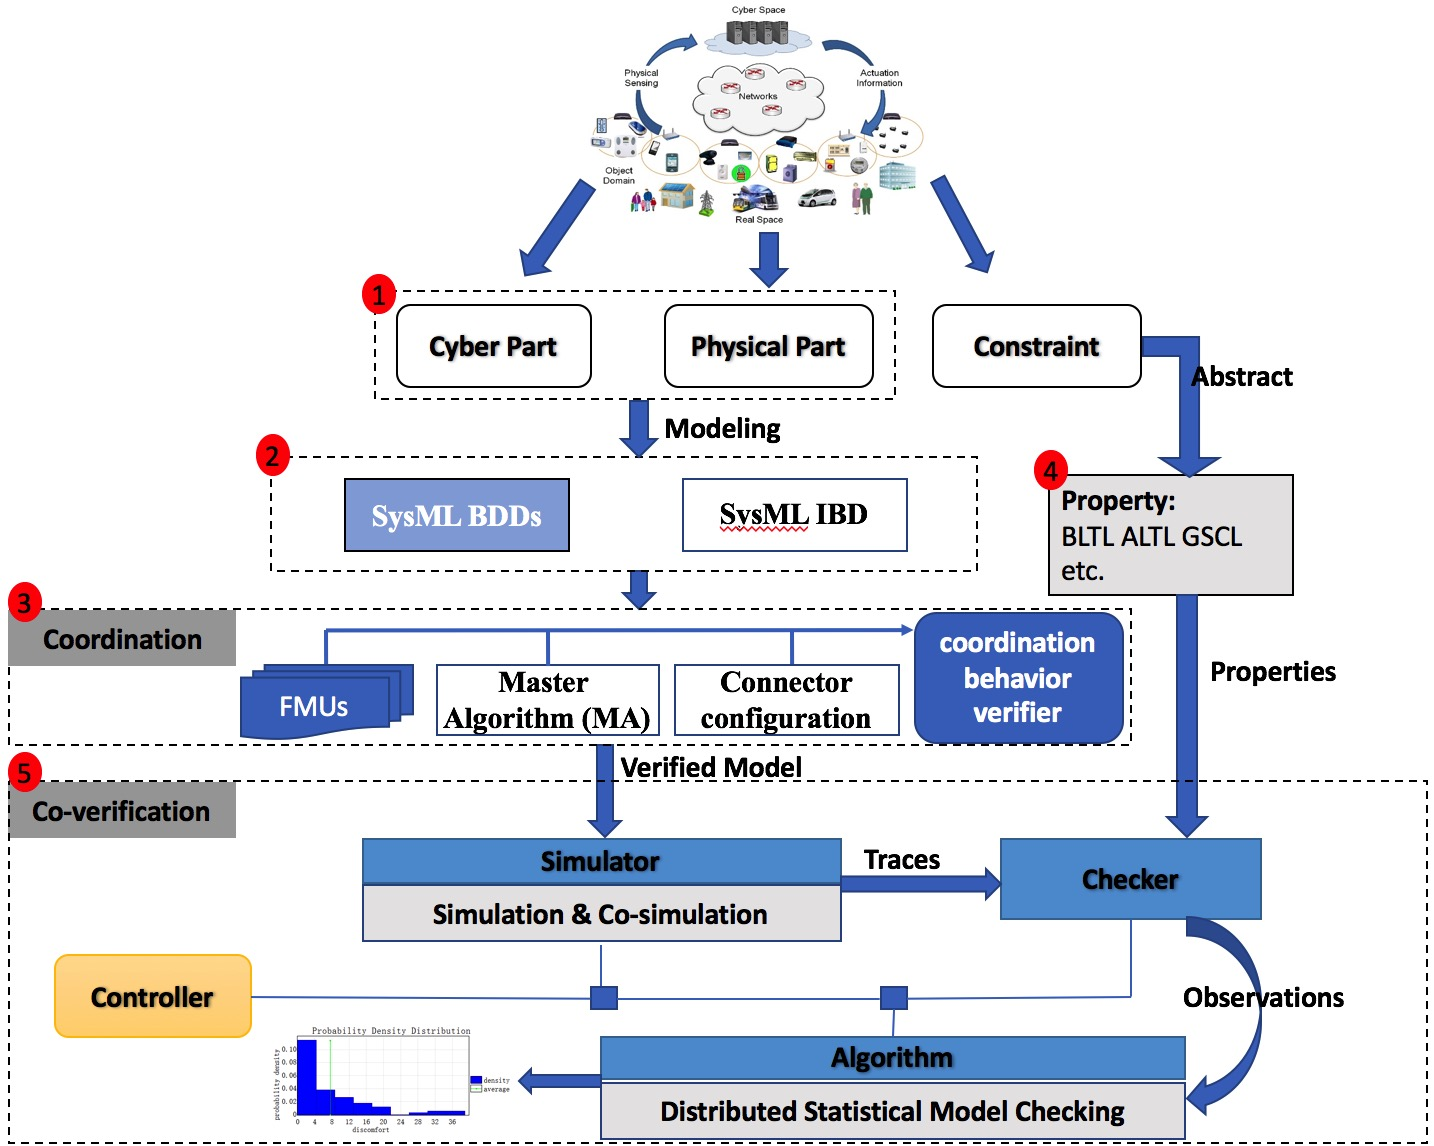
\includegraphics[width=6.0in]{fig/1/paper-framework.jpg}}
	%\vspace{0.10in}
	\caption{论文技术路线图}\label{pa-fra}
\end{figure}

\textbf{本文的具体研究内容和贡献点总结如下}:
\begin{enumerate}
	\item 使用SysML建模语言建模整个系统的架构,使用SysML的BDD图建模系统组件,使用SysML的IBD图来描述系统中各个组件的关联关系。
	\item 基于FMI标准实现SysML描述的系统模型,将SysML的BDD图建模的系统组件包装成FMU,并将各个组件的关联关系转化为FMU之间的接口配置文件。
    \item 使用时间自动机理论验证了基于FMI标准的多个组件的协同行为,使用时间自动机将协同仿真的主算法进行形式化描述,并使用UPPAAL \cite{•} 模型检测器来验证主算法的正确性;提出了一种从FMU到时间自动机的映射标准,通过此标准用时间自动机将多个FMU进行编码,并用时间自动机之间的通道(channel)来描述多个FMU之间的关联关系,最终将多个FMU及FMU之间的关联关系使用一个时间自动机网络进行了描述,将该时间自动机网络输入到UPPAAL之中进行验证从而来验证协同行为的正确性。
    \item 将验证属性用BLTL/ALTL/GSCL等形式化语言进行描述。
    \item 提出了一种基于抽象和学习的分布式统计模型检测算法,大大提高了统计模型检测的效率。
\end{enumerate}

\section{本文组织结构}
本文共分七章,组织结构如下:

第一章介绍了本文的研究背景及意义,并从四个方面阐述了该研究领域的国内外研究现状,其中包括信息物理融合系统的形式化建模、分布式技术、协同仿真及统计模型检测的研究现状。之后,给出了本文的技术路线和主要贡献点。最后,总结了论文组织结构。

第二章介绍了相关预备知识。首先给出了信息物理融合系统的主要概念,并详细讨论了我们本文关注的信息物理融合系统的异构性;之后,给出了概率有界线性时态逻辑和时间自动机的形式化描述,并给出了基于FMI标准的协同仿真通用接口。

第三章介绍了基于时间自动机理论来验证异构系统协同行为正确性的方法,首先我们给出了该方法的技术框架,之后我们详细描述了如何用时间自动机理论来验证协同仿真的主算法,以及如何验证整个异构系统的协同行为的正确性。

第四章重点阐述了如何用统计模型检测算法来对异构系统进行验证分析,也是本文的主要内容。首先,介绍了如何基于FMI标准对异构协同进行协同仿真并得到仿真迹,然后提出了一种基于抽象和学习的统计模型检测算法来提高统计模型检测的效率。最终,我们将协同仿真和该高效的统计模型检测算法进行结合,以此来对异构系统进行验证分析。

第五章主要介绍工具及程序实现。首先简单介绍了我们自己的CPS建模分析平台——Modana,之后给出了基于Modana平台的异构系统验证工具(Co-SMC工具)。最后,给出了Co-SMC工具的详细设计及程序实现。

第六章给出了两个案例,通过使用本文提出的方法对这两个案例进行建模、仿真和分析来验证本文提出方法的有效性。

第七章为总结和展望,总结了本文提出的基于分布式统计模型检测的异构系统验证方法,并讨论了其优点和不足,指出了未来要进一步进行研究的工作。
\section{本章小结}
本章首先说明了选题的背景和意义,指出了由于CPS的异构性而导致CPS系统的验证分析面临巨大挑战;接着介绍了信息物理融合系统的形式化建模、分布式技术、协同仿真及统计模型检测的研究现状;最后给出了本文的技术路线、主要贡献点和组织结构。下一章将介绍本文涉及到的预备知识及概念。

\chapter{预备知识与概念}
\label{ch2}
\section{功能模拟接口(FMI)}
CPS中各个组件之间的协同仿真可以基于FMI标准来实现,FMI标准最初是在2008年开始的MODELISAR项目中开发的,并得到大量软件公司和研究中心的支持。FMI支持模拟由异构组件组成的复杂系统,通过一个协同仿真环境将不同模型与自己的求解器耦合起来。实现了FMI标准接口的系统组件被称为FMU,我们可以基于FMI标准将模型转化为FMU,之后加入协同仿真的主算法就可以对系统进行协同仿真,其中主算法并不是FMI标准的一部分。FMI标准包含两个主要部分:
\begin{enumerate}
\item 协同仿真接口:一组用来实现对仿真器控制和完成多个FMU之间进行数据传输的C语言函数。
\item 协同仿真描述文件:用一个XML文件定义了模型的结构和主要的描述信息。主要包括模型的输入、输出信息,模型的仿真器和求解器等等。
\end{enumerate}
FMI至今已经有两个版本,即FMI1.0和FMI2.0\cite{Broman2013Determinate}。FMI1.0中有一个主要的函数是doStep,主函数可以调用该函数,使得FMI中的某个FMU进行一步的仿真。该函数的定义如下:\\
fmiStatus fmiDoStep( fmiComponent c, fmiReal currentCommunicationPoint, fmiReal communicationStepSize, fmiBoolean newStep); 

其中,$c$为主算法要调用的FMU组件,$currentCommunicationPoint$为主算法当前的仿真时间,$communicationStepSize$是主算法要FMU下一步进行仿真的步长。FMU接收到主算法的调用命令和调用步长时,将会接受或拒绝这一步长,如果接受这一步长则到进行仿真并到达一个新的状态,如果拒绝则需要重新调用。$newStep$用来表示当前的这一次仿真是一次新的调用还是拒绝之后的再次调用。

FMI2.0针对FMU1.0做了一定的扩展,主要是增加了$fmiGetFMUstate$和$fmiSetFMUstate$两个方法。这两个方法使得FMU可以对状态进行保存和恢复,从而支持了FMU状态的回滚。在后续章节,我们提出的支持回滚的主算法是基于这一扩展进行设计的。因此,扩展之后的doStep函数如下:\\
fmiStatus fmiDoStep(fmiComponent c, fmiReal currentCommunicationPoint, fmiReal communicationStepSize, fmiBoolean noSetFMUStatePriorToCurrentPoint);

其中,前三个参数跟FMU1.0里面的参数相同,只是最后一个参数的含义与FMI1.0有了本质的区别,通过设置$noSetFMUStatePriorToCurrentPoint$为true和false,主算法可以来控制FMU是否将之前一个状态的值设置给当前时间节点。
\section{功能模拟单元(FMU)}
我们在以上小节介绍了FMI标准接口,下面我们对实现了FMI标准接口的FMU给出形式化的语法和语义。
\begin{define}
\textbf{FMU 语法}

FMU的语法可以用一个八元组$F=(S,U,Y,D,s_{0},set,get,doStep)$表示,
\end{define}
\begin{itemize}
\item
$S$ 表示FMU的状态集合。
\item
$U$ 表示FMU的输入变量集合。
\item
$Y$ 表示FMU的输出变量集合。
\item
$D \subseteq U \times Y$ 表示多个FMU之间输入和输出之间的依赖关系集合。 $(u,y) \in D $表示输出变量$y$直接依赖于输入变量$u$的取值。 
\item
$s_{0} \in S$ 表示FMU的初始状态。
\item
$set : S \times U \times \mathbb{V} \rightarrow S$表示$set$函数对一个输入变量进行赋值。给定当前状态$s \in S$, 输入变量 $u \in U$及一个数值 $v \in \mathbb{V}$, 该函数将返回一个新的状态,此状态中$u$的值为$v$。
\item
$get : S \times Y \rightarrow \mathbb{V}$表示$get$函数返回某个输出变量的数值。给定一个状态 $s \in S$和一个输出变量$y \in Y$, $get(s,y)$返回$s$状态上$y$输出变量的取值。
\item
$doStep : S \times \mathbb{R}_{\geqslant{0}} \rightarrow S \times \mathbb{R}_{\geqslant{0}}$表示$doStep$函数进行了一步仿真。给定当前状态$s$和一个非负实数$h \in \mathbb{R}_{\geqslant{0}}$, $doStep(s,h)$返回一个元组$(s^{\prime},h^{\prime})$,且
\\
    当$h^{\prime} = h$时, $F$接受该步长并执行步长为$h$的仿真,并且迁移到了一个新的状态 $s^{\prime}$;
\\
    当$0 \leqslant h^{\prime} < h$时,$F$拒绝步长$h$,只执行步长为$h^{\prime}$的仿真,并且迁移到一个新的状态 $s^{\prime}$。
\end{itemize}
\begin{define}
\textbf{FMU 语义}
\end{define} 
给定一个FMU$F=(S,U,Y,D,s_{0},set,get,doStep)$,FMU的执行依赖于$doStep$函数,它的执行可以用一个时间输入序列(Timed Input Sequence, TIS)进行描述。TIS是一个有限的四元组序列$(t,s,v,v^{\prime})$, $t \in \mathbb{R}_{\geqslant{0}}$表示当前时刻,$s \in S$表示$F$的当前状态,$v$是一个输入变量,$v^{\prime} : Y \rightarrow \mathbb{V}$ 是一个输出变量。
 
TIS = $(t_{0},s_{0},v_{0},v_{0}^{\prime}), (t_{1},s_{1},v_{1},v_{1}^{\prime}),(t_{2},s_{2},v_{2},v_{2}^{\prime}), ..., (t_{i},$
$s_{i},v_{i},v_{i}^{\prime}), (t_{i+1},s_{i+1},v_{i+1},v_{i+1}^{\prime}), ...$定义如下:
\begin{itemize}
\item
$t_{0} = 0$时刻的$s_{0}$状态表示$F$处于初始状态位置。
\item
对于任意的$i \geqslant 1$, $t_{i} = t_{0} + \sum_{k = 1}^i h_{k}$。
\item
给定当前状态$s_{i}$,$set$函数用来将当前状态的输入参数设置为一个特定的数值$v$,之后$F$执行$doStep$函数并且迁移到一个新的状态$s_{i}^{\prime}$。$get$函数用来得到当前状态的所有输出参数的取值$v_{i}^{\prime}$。
\end{itemize}
\section{时间自动机(TA)}
时间自动机\cite{BehrmannDLHPYH06}是一个建模实时系统行为的经典理论模型。 在本小节中,我们给出时间自动机的形式化语法和语义。
\begin{define}
\textbf{时间自动机 语法}

时间自动机可以用一个四元组$\textit{A}=(L,l_{0},E,I)$来表示,其中:
\end{define}
\begin{itemize}
\item
$L$表示时间自动机中有限的位置集合;
\item
$l_{0} \in  L$为时间自动机的初始位置;
\item
约束集合$G(x)$可以用$g = x \bowtie c \mid g \land g$来表示,其中 $x \in X$, $c \in \mathbb{N}$且$\bowtie~\in \{<,\leqslant,\geqslant,>,=\}$。
\item
$E \subseteq L \times G(X) \times Act \times 2^X \times L$是一组边的集合, 该边包含约束和时钟,其中 $Act = Act_{i} \cup Act_{o}$。$Act_{i}$是一个输入动作的集合,$Act_{o}$是一个输出动作的集合。
\item
$I : L \rightarrow G(X)$将不变量指定给位置。
\end{itemize}
\begin{define}
\textbf{时间自动机语义} 

时间自动机$\textit{A}=(L,l_{0},E,I)$的语义可以用一个标签迁移系统$L_{\textit{A}} = (Proc,Lab,\lbrace {{\xrightarrow{\alpha}}} \mid \alpha \in Lab \rbrace)$进行描述,其中:
\end{define}
\begin{itemize}
\item 
$Proc = \lbrace(l,v) \mid (l,v) \in L \times (X \rightarrow \mathbb{R}_{\geqslant{0}})$且$v \models I(l) \rbrace$,其中状态是一个$(l,v)$元组,$l$是时间自动机中的位置且$v$是满足$I(l)$的一个时钟变量;
\item
$Lab = Act \cup \mathbb{R}_{\geqslant{0}}$ 是一个标签集合;
\item
迁移关系定义如下:

$(l,v) \xrightarrow{\alpha} (l^{\prime},v^{\prime})$,如果存在一个边 $(l \xrightarrow{g,\alpha,r} l^{\prime}) \in E$,则$v \models g$, $v^{\prime} = v[r]$且$v^{\prime} \models I(l^{\prime})$

$(l,v) \xrightarrow{d} (l,v+d)$,对于所有的$d \in  \mathbb{R}_{\geqslant{0}}$,则$v \models I(l)$且$v + d \models I(l)$
\end{itemize}
对于时间自动机$A$中某个位置$l$的可达性问题就是一个判断在迁移系统$L_{A}$中是否存在一个从初始状态$(l_{0},v_{0})$到状态$(l,v)$的路径。为了验证需要,我们定义了时间自动机的符号语义,该定义用到了一组包含时钟的执行序列集合。

对于一个特定的位置$l$和特定的时刻 $t \in X$,对于任意的$x \in X$,则$t + x \in X$。从该时刻位置开始的执行序列如下所示:

$(l,t) \xrightarrow{x_{1}} (l,t+x_{1}) \xrightarrow{x_{2}} (l,t+x_{1}+x_{2}) \xrightarrow{x_{3}} (l,t+x_{1}+x_{2}+x_{3}) \xrightarrow{x_{4}}...\xrightarrow{x_{i}}(l,t+x_{1}+x_{2}+x_{3}+...+x_{i}) \xrightarrow{x_{i+1}}...$

其中$x_{i} > 0$且无穷序列$x_{1} + x_{2} + . . .$ 对于$x$是收敛的。 
\section{系统建模语言(SysML)}
SysML是为模型驱动式软件开发(Model-Based Systems Engineering,MBSE)\cite{Dori16}而提出的一种通用的领域建模语言( Domain-Specific Language,DSL)\cite{SemerathBHSV17} ,它起源于国际系统工程委员会(INCOSE)的倡议\ cite {Pepper2015International}并于2001年1月发布 。SysML基于统一建模语言2.0(Unified Modeling Language2.0,UML2.0)\cite{Bjerkander2003Architecting}的一个子集,加入了其他一些建模元素的扩张。SysML的提出是用来统一复杂系统开发的各种建模语言和技术。SysML是一种基于UML建模语言,针对系统工程做了相应的扩展而构造出的一种建模语言。它为系统的建模和需求建模提供了新的方法。 在\cite{Bjerkander2003Architecting}中,Willard B.重点介绍了UML2.0的发展,并提出了SysML带来的新的可能性,他声称SysML的主要优点是“为系统工程师提供标准和全面的系统规范范例”。 SysML使用UML2.0中的图作为类或对象图,但是采取了新的语义来避免软件词汇表(例如,类和对象被块代替)。此外,加入新的图来简化需求的声明,并针对之后的仿真提出了一些相关的设计。块(block)是SysML的基本概念。 块是描述系统的每个模块单元的基本建模元素。 块定义了一组代表组件结构和行为的特征和操作。 这些块在BDD内以层级关系进行声明和组织。 在BDD中,块拥有自己的属性,这些属性将它们的特征和子元素定义为部件和端口。此外,块还拥有它们能够执行的一组操作。IBD则显示了各个块的端口之间的连接关系。

\section{概率有界线性时态逻辑(PBLTL)}
概率有界线性时态逻辑(Probabilistic Bounded Linear Temporal Logic,PBLTL)\cite{David2012Statistical}公式可以用来形式化的描述系统的验证属性。我们先给出有界线性时态逻辑(Bounded Linear Temporal Logic,BLTL)的语法和语义,然后再将其扩展为PBLTL。

给定一个模型$M$,设其状态变量的集合$SV$是一个有限的实数集,在$SV$上的一个布尔谓词约束为$y \sim v$形式。其中$y\in SV$,$\sim \in \lbrace \geq,\leq,=\rbrace$且$v\in \mathbb{R}$。BLTL的语法定义如下:
$$\varphi ::= y \sim v\mid\phi_{1}\wedge\phi_{2}\mid\phi_{1}\vee\phi_{2}\mid \neg \phi_{1}\mid\phi_{1}U^{\leq t}\phi_{2}
$$
其中,$\sim \in \lbrace \geq,\leq,=\rbrace$,$y\in SV$,$v\in \mathbb{Q}$,$t\in \mathbb{Q}_{\geq 0}$。

定义算子“$F$”表示最终会满足,$F^{\leq t}\phi = True U^{\leq t}\phi$,表示最终在$t$时间内存在$\phi$满足;

定义算子"$G$"算子表示始终满足,$G^{\leq t}\phi = \neg F^{\leq t}\neg \phi$,表示在$t$时间内$\phi$始终满足。

对于一条仿真迹$\sigma$,$\sigma^k$表示$\sigma$从第$k$步开始执行之后的部分。我们规定$V(\sigma,k,y)$表示迹 $\sigma$在第$k$步时状态变量$y$的值,$t_k$表示第$k$步需要的时间,$t$表示时间约束,则BLTL在迹$\sigma^k$上的语义定义如下:

\begin{define}\label{def:bltl_semantics}
(有界线性时态逻辑的语义).	
\begin{itemize}
\item $\sigma^{k}\vDash y \sim v $当且仅当$V(\sigma,i,y)\sim v$。
\item $\sigma^{k}\vDash\phi_{1}\vee\phi_{2}$当且仅当$\sigma^{k}\vDash\phi_{1}$或$\sigma^{k}\vDash\phi_{2}$。
\item $\sigma^{k}\vDash\phi_{1}\wedge\phi_{2}$当且仅当$\sigma^{k}\vDash\phi_{1}$且$\sigma^{k}\vDash\phi_{2}$。
\item $\sigma^{k}\vDash\neg\phi_{1}$当且仅当$\sigma^{k}\vDash\phi_{1}$不成立。
\item $\sigma^{k}\vDash\phi_{1}U^{t}\phi_{2}$当且仅当存在数值$i$使得

$ \Sigma_{0\leq l<i}$ $t_{k+1}\leq t$;

$ \sigma_{k+i}\models\phi_{2}$;

$\sigma_{k+j}\models\phi_{1}$,对于每个$ 0\leq j \leq i$。
\end{itemize}
\end{define}

\begin{define}\label{def:pbltl}
(概率有界线性时态逻辑).

一个PBLTL属性公式$\phi$可以表示为$P_{\geq \theta}(\phi')$,其中$\phi'$为BLTL公式,$\theta$为一个阈值(介于0和1之间)。对于定性分析的PBLTL验证属性,我们将其表示为$M \models P_{\geq \theta}(\phi)$,即来验证模型$M$满足BLTL属性$\phi'$的概率是否不小于$\theta$。对于定量分析的PBLTL验证属性公式,无需指定阈值$\theta$,可以将其表示为$M \models P_{=?}(\phi')$,即来验证模型$M$满足BLTL属性$\phi'$的概率是多少。
\end{define}


\section{本章小结}
本章首先介绍了实现异构系统各个组件之间协同运行的标准,即FMI标准和FMU的语法及语义;同时,给出了用于验证组件之间协同行为正确性的理论模型-时间自动机的语法和语义。最后,给出了描述本文的验证属性主要用到的逻辑公式PBLTL的语法和语义。下一章我们将介绍如何建模整个异构系统的架构以及如何基于时间自动机理论来验证异构系统中各个组件协同行为的正确性。

\chapter{异构系统协同行为的正确性验证}
\label{ch3}
在本章节,我们首先用SysML建模语言对整个异构系统的架构进行建模,其中用SysML的BDD图来建模系统的组件,用SysML的IBD图来建模系统中各个组件之间的关联关系。由于SysML只是用来建模系统的架构,该建模语言得到的模型不可执行。因此,我们基于FMI标准,将SysML的BDD描述的组件用FMU进行实现,将SysML的IBD图转化为FMU之间的接口配置文件。因此,我们只需要设计协同仿真主算法就可以完成异构系统基于FMI的协同仿真。然而,在我们将基于FMI的可仿真模型输入到协同仿真引擎之中进行仿真之前,我们需要确保该模型的协同行为的正确性,即要保证该模型可以正确的进行协同仿真。为了解决这个问题,我们需要进行两个方面的验证:(1)我们要验证协同仿真主算法的正确性,即算法没有出现死锁以及其他一些特性;(2)我们要验证系统之间各个组件之间关联顺序及数据交互的正确性,其中最主要的要保证多个FMU没有出现环路依赖。由于FMU的执行时基于时间的,而时间自动机在建模时间有较大的优势,且时间自动机的验证有着良好的工具支持,因此,在接下来的内容中,我们重点描述如何基于时间自动机理论来验证整个可仿真模型的协同行为的正确性。在第一小节,我们给出整个验证过程的技术框架;第二小节介绍如何对上述的第一个方面进行验证,即协同仿真的主算法的验证;在第三小节中,我们使用一个具体的案例来描述如何对上述的第二个方面进行验证,即异构系统协同行为的验证。
\section{技术框架}
\begin{figure}[htbp]
	\centering
	{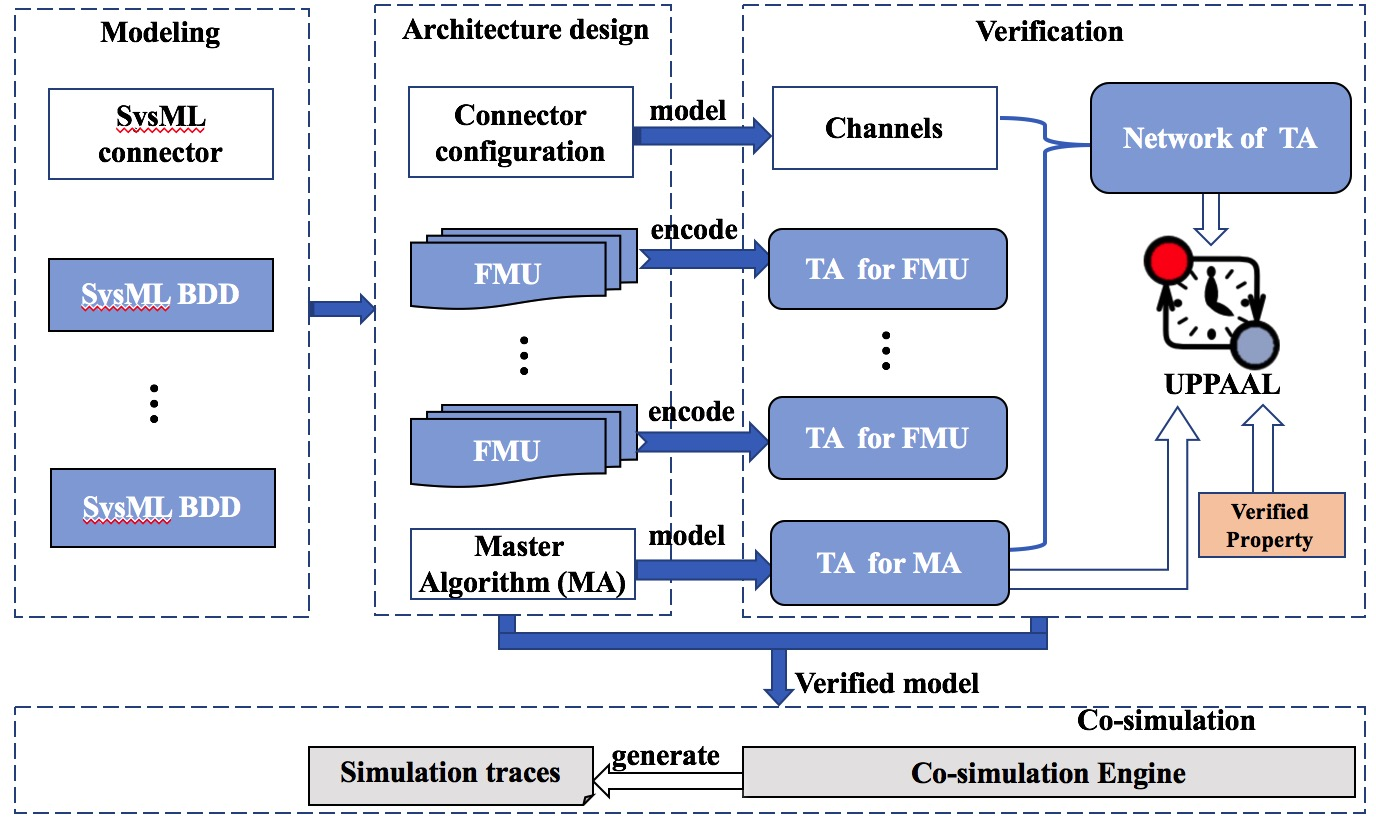
\includegraphics[width=6.0in]{fig/3/framework-3.jpg}}
	%\vspace{0.10in}
	\caption{协同行为正确性验证技术框架图}\label{fra-3}
\end{figure}
图\ref{fra-3}为异构系统协同行为正确性验证的技术框架图. 首先,我们在建模(Modeling)阶段使用SysML的BDD和IBD图来建模整个异构系统的架构。SysML的BDD中的块建模了异构系统的一个个组件;SysML的IBD图描述了各个块之间的连接关系。为了借助协同仿真技术对整个系统进行协同仿真,我们在架构设计(Architecture design)阶段将一个个块用FMU进行实现,同时将IBD图描述的关联关系转化为一个FMU之间的配置文件(Connector configuration)。接下来,我们自己设计了协同仿真的主算法(Master Algorithm,MA)来实现各个FMU之间的交互,同时来驱动协同仿真过程的执行。接下来是协同行为的验证(verification)阶段,也是我们本文的主要贡献点之一。为了验证协同行为的正确性,(1)我们先验证了协同仿真主算法的正确性:首先,我们用时间自动机对协同仿真的主算法进行形式化建模,然后将该时间自动机模型输入到UPPAAL模型检测工具中进行验证 (2)我们验证了整个系统协同行为的正确性:我们提出了一种从FMU到时间自动机的映射规则,我们根据此规则将FMU映射为时间自动机,接下来将FMU之间的配置文件转化为时间自动机的通道(Channels)。这样,我们就得到了一个时间自动机网络(Network of
TA):包括FMU映射成的时间自动机、主算法的时间自动机及各个时间自动机之间的通道)。最后我们将该时间自动机网络和要验证的属性(死锁、可达性、活性等)输入到UPPAAL中来验证该模型是否满足某些属性。一旦验证了协同行为的正确性,我们就可以将通过验证的模型输入到协同仿真的引擎之中进行协同仿真并得到协同仿真的迹。接下来,我们将详细介绍整个协同行为的验证过程。
\section{协同仿真主算法的验证}
在本小节我们首先介绍了三种协同仿真的主算法:固定步长算法、可回滚算法及可预测步长算法,之后我们用时间自动机形式化建模了这几种算法,最后将这几种算法的形式化模型输入到UPPAAL工具中,分别验证了这几种算法的有无死锁、可达性和活性的属性。
\subsection{协同仿真主算法介绍}
协同仿真的主算法用了调度和协同异构系统的多个	FMU组件的执行。每一个FMU都可以被看做一个可独自仿真的黑盒,但是多个FMU之间在某些特定的时刻需要进行数据交互和同步。图\ref{ad-fixedstep}描述了当前三种主要的协同仿真主算法的活动图。在接下来的内容中,我们对这三种算法进行简单的介绍。
\begin{figure}[htbp]
\centering{
		\subfigure[固定步长算法]{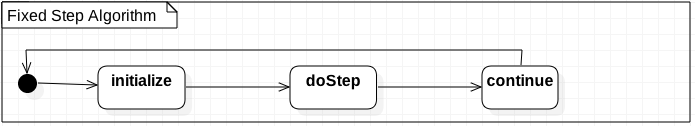
\includegraphics[width=4.5in,height=0.8in]{fig/3/MA1.png}
			\label{sd_fixedstep}}
		\hfil
		\subfigure[可回滚算法]{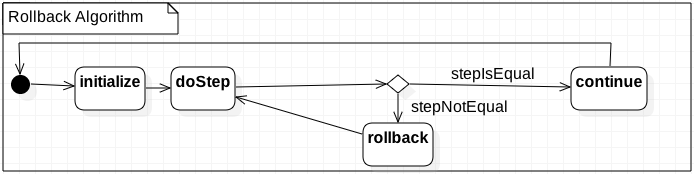
\includegraphics[width=4.5in,height=0.9in]{fig/3/MA2.png}
			\label{sd-rollback}}	
		\subfigure[可预测步长算法]{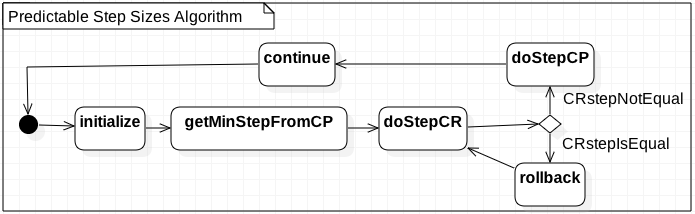
\includegraphics[width=4.5in,height=1.1in]{fig/3/MA3.png}
			\label{sd-pre}}		
	\caption{三种协同仿真主算法的活动图}
	\label{ad-fixedstep}
	}
\end{figure}
\subsubsection{固定步长算法}
对于固定步长算法\cite{BromanBGLMTW13},所有的FMU都有一个相同的步长。当协同仿真主算法在$t$时刻调用$doStep$函数执行步长$h$时,所有的FMU将从$t$时刻执行$h$步长并到达$t+h$时刻。在执行下一个$doStep$函数之前,要确保所有的FMU都执行完了上一个步长并且完成了数据交换。固定步长算法的活动图如图\ref{sd_fixedstep}所示,该活动图主要包含三个活动: $initialize$, $doStep$ 和 $continue$,首先对所有的FMU进行初始化,之后调用$deStep$函数进行仿真,最后在$continue$活动中完成FMU的数据交换。 在固定步长算法中,只要保证每个FMU的仿真是可靠的,则可以保证整个仿真过程的可靠性。但是,如果在某个FMU的仿真过程中出现错误,则会导致整个协同仿真过程出错。为了克服固定步长算法的缺陷,出现了可回滚的算法。
\subsubsection{可回滚算法}
FMI2.0相对于FMI1.0添加了几个重要的特性,它支持了对于FMU状态的保存和回滚。例如,主算法调用$FMU_{1}$和$FMU_{2}$的$doStep$函数执行$h$步长,但是$FMU_{1}$接受了该步长且$FMU_{2}$拒绝了该步长,则$FMU_{1}$和$FMU_{2}$都会执行$h$步长然后回滚到上一个时间点。可回滚算法的活动图如图\ref{sd-rollback}所示,相比固定步长算法,可回滚算法要求所有的FMU支持$rollback$方法, 且当某个FMU拒绝该步长时,所有的FMU将会回滚到上一个步长执行完之后的时间点。
\subsubsection{可预测步长算法}
如果可以预测FMU下一步能执行的最大步长(FMU在不错过事件时,能执行的仿真的最长时间),则可以大大提高协同仿真的效率。因此,论文\cite{BromanBGLMTW13}提出了$GetMaxStepSize$函数来预测FMU下一步能执行的最大步长,有了该函数的支持,就出现了可预测步长算法。图\ref{sd-pre}为可预测步长算法的活动图,首先,所有的FMU进行初始化,然后支持$GetMaxStepSize$函数的FMU在$getMinStepFromCP$活动中预测他们下一步能执行的最大步长,并且在所有的最大步长中选择最小的一个$h$作为所有FMU下一步执行的步长,之后所有的FMU执行$h$步长,如果所有的FMU都接受了该步长,则所有的FMU仿真该步长然后进行下一步。如果有FMU拒绝了该步长,则将所有的FMU回滚到上一个时间点,然后选择一个更小的步长进行仿真。
\subsection{协同仿真主算法的建模和验证} 
\label{sec:ma}
我们用时间自动机将三种不同类型的主算法进行形式化建模,图\ref{ta-master}是三种主算法的时间自动机模型。固定步长算法的时间自动机模型包含$Init$和$doStep$两个状态,且与$FMU$通过$continue$信道进行通信。 可回滚算法包括$Init$、$DoStep$和$Continue$三个状态。如果所有的FMU都接受了下一步要进行仿真的步长,则可回滚算法对应的时间自动机将发送$continue$信号,且迁移到$Continue$状态;否则,将发送$rollback$信号,且返回到上一个状态。可预测步长算法包括$Init$, $find \_ CP \_ MIN$, $DoStep$, $writeCP$四个状态。首先他们获得支持预测步长算法的多个FMU的最大步长,然后取所有最大步长的最小值$step1$ 。然后执行该步长,如果所有的FMU都接受则发送$continue$信号并迁移到下一个状态,否则发送$rollback$信号并回滚到$DoStep$ 状态。
\begin{figure}[htbp]
\centering{
		\subfigure[固定步长算法的时间自动机模型]{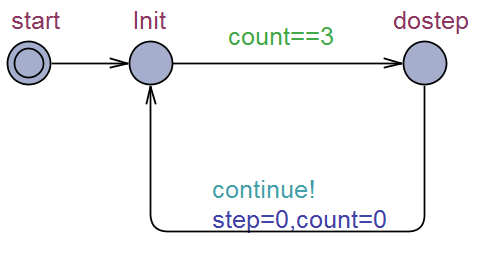
\includegraphics[width=1.5in,height=1.0in]{fig/3/fixedstep_master.png}
			\label{ta_fixedstep}}
		\hfil
		\subfigure[可回滚算法的时间自动机模型]{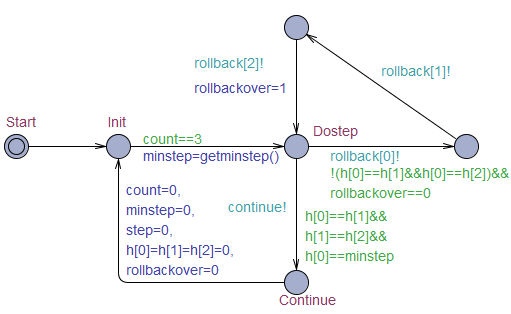
\includegraphics[width=2.5in,height=1.3in]{fig/3/rollback_master.png}
			\label{ta-rollback}}	
		\subfigure[可预测步长算法的时间自动机模型]{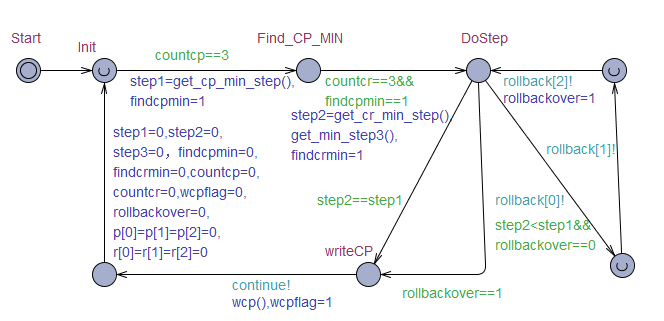
\includegraphics[width=4.5in,height=1.5in]{fig/3/pma_master.png}
			\label{ta-pre}}		
	\caption{三种不同主算法的时间自动机模型。}
	\label{ta-master}
	}
\end{figure}

UPPAAL是基于时间自动机理论对实时系统进行验证的工具,其中使用到的时间自动机模型增加了整型变量、多种数据类型及同步信号等扩展。我们使用UPPAAL工具验证了这三个模型的可达性、活性及死锁。具体的验证属性如下所示:
\begin{itemize}
\item
$E \langle\rangle master.dostep$, $E\langle\rangle master.Continue$ and $E\langle\rangle master.writeCP$是可达性验证,用来验证这些系统状态是否可达;
\item
$master.Init -> master.dostep$, $master.Init -> master.Continue$ and $master.Init -> master.Continue$是活性验证。如果主算法可以到达前一个状态,那么它最终也会到达后一个状态。
\item
$A[] not deadlock$ 是死锁的验证, 用来验证主算法是否存在死锁。
\end{itemize}
实验的结果如表\ref{ta_r}所示,从表中我们可以看出不存在死锁,且可达性和活性都满足,说明我们的主算法是正确的。例如:属性$A[]~not~deadlock$满足,说明主算法不存在死锁; 属性$E\langle\rangle~master.doStep$ 满足,说明系统最终会到达$doStep$状态。 总结来说,我们在这一小节验证了我们所用到的协同仿真的主算法的正确性。
\begin{table}
\caption{主算法的验证实验结果}
\centering
\begin{tabular}{c c c}
          \hline
          主算法 & 验证属性 & 结果\\
       \hline
        \multirow{2}{2.0cm}{固定步长}
                & $A[]~not~deadlock$ & True\\
                & $master.Init -> master.dostep$ & True\\
                & $E\langle\rangle~master.dostep$ & True\\

        \hline
        \multirow{2}{2.0cm}{可回滚}
                & $A[]~not~deadlock$ & True\\
                & $master.Init -> master.Continue$ & True\\
                & $E\langle\rangle~master.Continue$ & True\\

        \hline
        \multirow{2}{2.0cm}{可预测}
                & $A[]~not~deadlock$ & True\\
                & $master.Init -> master.writeCP$ & True\\
                & $E\langle\rangle~master.writeCP$ & True\\
        \hline
\end{tabular}
\label{ta_r}
\end{table}

\section{异构系统协同行为的验证}
在本小节,我们使用一个水箱的案例对整个协同行为的验证过程进行详细的描述。由于,在验证过程中,需要用时间自动机对FMU进行形式化描述,我们首先给出了从FMU到时间自动机的映射规则,然后我们使用SysML对整个系统进行架构设计,之后基于FMI标准对系统的各个组件进行实现,并给出多个FMU之间的连接关系配置,最后我们用时间自动机建模了FMU的形式化模型,并输入到UPPAAL工具中针对验证属性进行验证分析。
\subsection{FMU到时间自动机的映射} 
\label{sec:encode}
在本文的第二章的预备知识中,我们给出了FMU和时间自动机的语法及语义,下面我们根据第二章的语法语义给出FMU和时间自动机的映射关系。我们发现FMU和时间自动机的语义之间存在一定的关联。FMU的语义关注于FMU的执行序列,也就是状态随着时间的不断迁移;因此,时间自动机的执行迹跟FMU的执行序列十分相似,也是状态随着时间的迁移序列。因此,我们使用时间自动机来对FMU进行形式化描述,从而来分析多个FMU之间的协同行为。
给定一个FMU$F=(S,U,Y,D,s_{0},set,get,doStep)$, 我们可以根据他们执行语义之间的关联,将FMU用时间自动机$\textit{A}=(L,l_{0},E,I)$进行形式化描述:
\begin{itemize}
\item
$L$是时间自动机的有限位置集合。因此,时间自动机语义模型$L_{\textit{A}}$中的状态可以看做为FMU中的状态,即$(l,v) \Rightarrow s$。
\item
时间自动机语义模型$L_{\textit{A}}$中的初始状态可以看做为FMU中的初始状态, 即$(l_{0},v_{0}) \Rightarrow s_{0}$。
\item
FMU中的输入变量$u \in U$可以看做为时间自动机的$Act_{i} \cup \{absent\}$。
\item
FMU的输出变量$y \in Y$可以看做为时间自动机的$Act_{o} \cup \{absent\}$。
\item
时间自动机的输入动作$e \in Act_{i}$可以看做FMU中的$set$函数。
\item
时间自动机的输出动作$e \in Act_{o}$可以看做为FMU中的$get$函数。  
\item
时间自动机之间依靠channel的同步可以看做为FMU之间的依赖关系。 $(u,y) \in D$表示输出变量$y$依赖于输入变量$u$,在时间自动机中输出动作同样依赖于输入动作。
\item
对于时间自动机,一个动作$e \in Act$会触发一个迁移$s \xrightarrow{e} s^{\prime}$, 这个过程就相当于FMU里面的$doStep$执行,会使其到达下一个状态。 例如:时间自动机的迁移$l \xrightarrow{e} l^{\prime}$可以描述FMU的$doStep(s,h)$被调用,并且此FMU接受了步长$h$并到达了下一个状态 $s^{\prime}$;然而,此FMU也可能会拒绝步长$h$, 并且发生了回滚,这个过程在时间自动机里面可以用一条边$l^{\prime} \xrightarrow{e} l$来进行描述,来表示回滚到了上一个状态。

\end{itemize}
\begin{figure}[htbp]
	\centering	{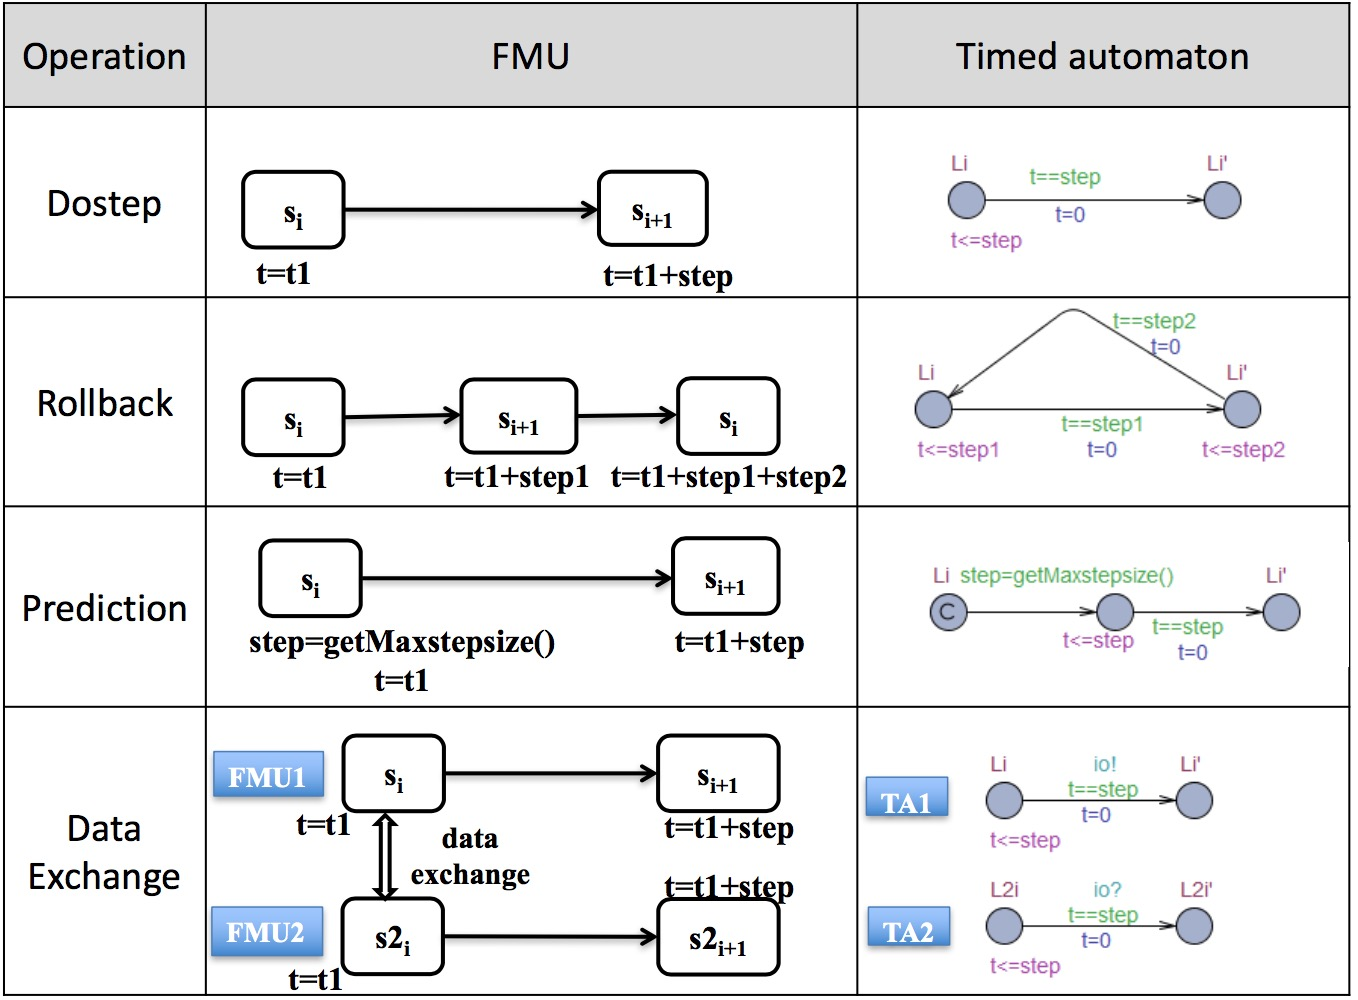
\includegraphics[width=5.0in,height=3.5in]{fig/3/abstractRole.png}}
	\caption{Encoding rules from FMU to TA.}
	\label{fmutota}
\end{figure}

将FMU直接转化为时间自动机是比较难得,S. Tripakis层在论文 \cite{Tripakis15}中将时间自动机编码为FMU。我们受到此论文的启发,根据时间自动机和FMU之间语义的关联,提出了几条从FMU到时间自动机在操作语义上的映射规则如图\ref{fmutota}所示。

给定FMU$t_{1}$时刻的当前状态$s_{i}$,操作函数$Dostep$可以使得FMU在$t_{1}+step$时刻到达$s_{i+1}$状态。这个操作可以用时间自动机的迁移来进行表示:在位置$L_{i}$延迟$step$的时间并迁移到一个新的位置$L_{i}^{\prime}$。

对于操作函数$Rollback$,给定FMU$t_{1}$时刻的当前状态$s_{i}$,FMU首先执行步长$step1$并在 $t_{1}+step1$时刻到达$s_{i+1}$状态,然后操作函数$rollback$又使得FMU回滚到上一个状态$s_{i}$。对于时间自动机来说,这个可以表示为在$L_{i}$位置延迟了$step1$时间单位并迁移到新的位置 a$L_{i}^{\prime}$,之后又迁移到了上一个位置$L_{i}$。 

对于操作函数$Prediction$,给定一个状态$s_{i}$, FMU可以由一个函数$getMaxstepsieze$得到下一步能执行的最大步长,然后执行此步长并在$t_{1}+step$时刻到达 $s_{i+1}$状态。 对于时间自动机,可以表示为在$L_{i}$位置执行了一个函数并得到要延迟的时间 $step$, 然后延迟该时间单位并迁移到一个新的位置 $L_{i}^{\prime}$ .

对于操作函数$Data Exchange$,两个FMU在$t_{1}$时刻的$s_{i}$状态执行$Data Exchange$进行了数据交换, 然后他们执行相同的步长并迁移到下一个位置$s_{i+1}$和$s2_{i+1}$。对于时间自动机,可以表示为两个时间自动机在$t_{1}$时刻通过信道$io$进行了同步,然后延迟了相同的时间并$L_{i}$位置迁移到$L_{i+1}$位置。

为了将FMU用时间自动机进行形式化描述,我们提出了以上操作语义的映射规则。为了证明我们以上规则的正确性,我们分析了FMU和时间自动机的执行片段如下所示:
\begin{itemize}
\item
对于操作函数$Dostep$的映射,在FMU和时间自动机中的执行片段为 ($s_{i}$, $t_{1}$), ($s_{i+1}$, $t_{1}+step$)和($l_{i}$, $t$), ($l_{i}^{\prime}$, $t+step$). 这说明时间自动机和FMU都执行 $step$的时间单位并到达了一个新的状态或是位置。
\item 
对于操作函数$Rollback$的映射, 在FMU和时间自动机的执行片段为($s_{i}$, $t_{1}$), ($s_{i+1}$, $t_{1}+step1$), ($s_{i}$, $t_{1}+step1+step2$) 和 ($l_{i}$, $t$), ($l_{i}^{\prime}$, $t+step1$), ($l_{i}$, $t+step1+step2$)。这说明时间自动机和FMU都首先执行了$step1$时间单位,并且到达了一个新的状态或位置,然后执行了$step2$时间单位, 又返回到了之前的状态或位置。
\item
对于操作函数$Prediction$的映射,FMU和时间自动机的执行片段为($s_{i}$, $t_{1}$), ($s_{i+1}$, $t_{1}+step$)和($l_{i}$, $t$), ($l_{i}^{\prime}$, $t+step$). 这说明时间自动机和FMU都成功预测到了步长$step$并执行了此步长。
\item
对于操作函数$Data Exchange$的映射,FMU1和时间自动机TA1的执行片段为 ($s_{i}$, $t_{1}$), ($s_{i+1}$, $t_{1}+step$)和($l_{i}$, $t$), ($l_{i}^{\prime}$, $t+step$)。FMU2和时间自动机TA2的执行片段为 ($s2_{i}$, $t_{1}$), ($s2_{i+1}$, $t_{1}+step$) 和 ($l2_{i}$, $t$), ($l2_{i}^{\prime}$, $t+step$)。这说明时间自动机和FMU在经过了数据交换后又执行了$step$时间单位。
\end{itemize}
为了更加准确的验证映射规则的正确性,我们分析了时间自动机和FMU的整个执行序列。我们通过分析得到FMU和时间自动机的执行序列是等价的,验证了映射规则的正确性。在之后几个小节的内容中,我们将此映射规则应用到了水箱的案例中,根据我们之后对案例仿真片段的分析,我们也发现映射规则是正确的。 
\subsection{基于SysML的架构建模} 
为了更好的阐述我们的方法,我们采用了水箱的案例 \cite{•} 作为驱动以更加形象的展示我们的方法。下面我们先简单的介绍一下水箱案例,然后用SysML建模语言对整个案例的架构建模。水箱案例:有一个水源可以向水箱里面注水,且水箱里面的水通过一个管道流入到一个水池当中,这个水源的流出由一个阀门控制,而阀门的开关由一个控制器进行控制。在本小节,由于水箱、阀门、控制器连接方式的不同,我们在此描述了三种不同类型的水箱系统。

SysML是为模型驱动式软件开发(Model-Based Systems Engineering,MBSE)\cite{Dori16}而提出的一种通用的领域建模语言( Domain-Specific Language,DSL)\cite{SemerathBHSV17} ,它起源于国际系统工程委员会(INCOSE)的倡议\ cite {Pepper2015International}并于2001年1月发布 。SysML的BDD图用块来描述系统中组件的结构;IBD图用来描述各个块之间的关联关系。各个块的接口由连接器进行关联,因此,系统各个组件的依赖关系可以用各个块的接口之间的连接进行表示。

图\ref{myad}是水箱案例的SysML BDD图,其中包含三个块: $Valve$, $Tank$ 和 $Controller$。 $Valve$和$Tank$是物理组件;$Controller$是信息组件。每一个组件都有自己的输入和输出接口,例如:$Valve$的输入接口是$vin$,它用来输入阀门的开关$OpenClosed$信号。
\begin{figure}[htbp]
	\centering	{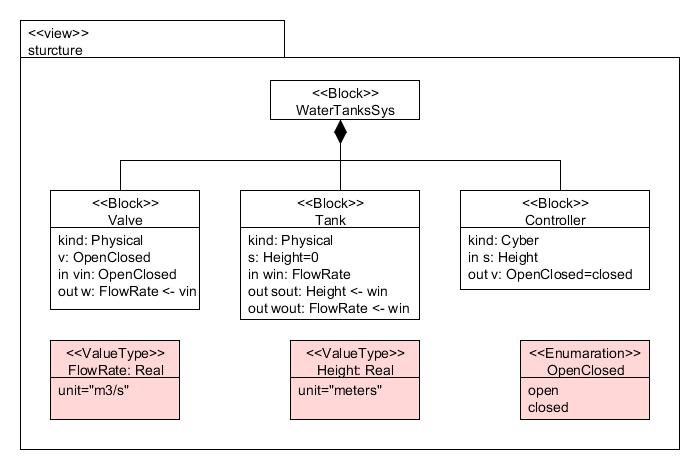
\includegraphics[width=4.5in,height=3.0in]{fig/3/AD.jpg}}
	\caption{水箱系统的SysML BDD}
	\label{myad}
\end{figure}

图\ref{cd} 是SysML的IBD图,在这里我们给出了三种连接情形。在第一种情形中,系统包含一个阀门、一个控制器和一个水箱,控制器随机的给阀门发送开关信息,导致水箱中的水位不断的变化;在第二种情形中,控制器信号的发送受到水箱水位的影响,控制器根据水箱的水位发送开关信号;在第三种情形中,我们添加了一个水箱$waterTank2$,水箱$waterTank1$中的水通过管道先流入$waterTank2$中,最后流入水池。

\begin{figure}[htbp]
\centering{
		\subfigure[情形1]{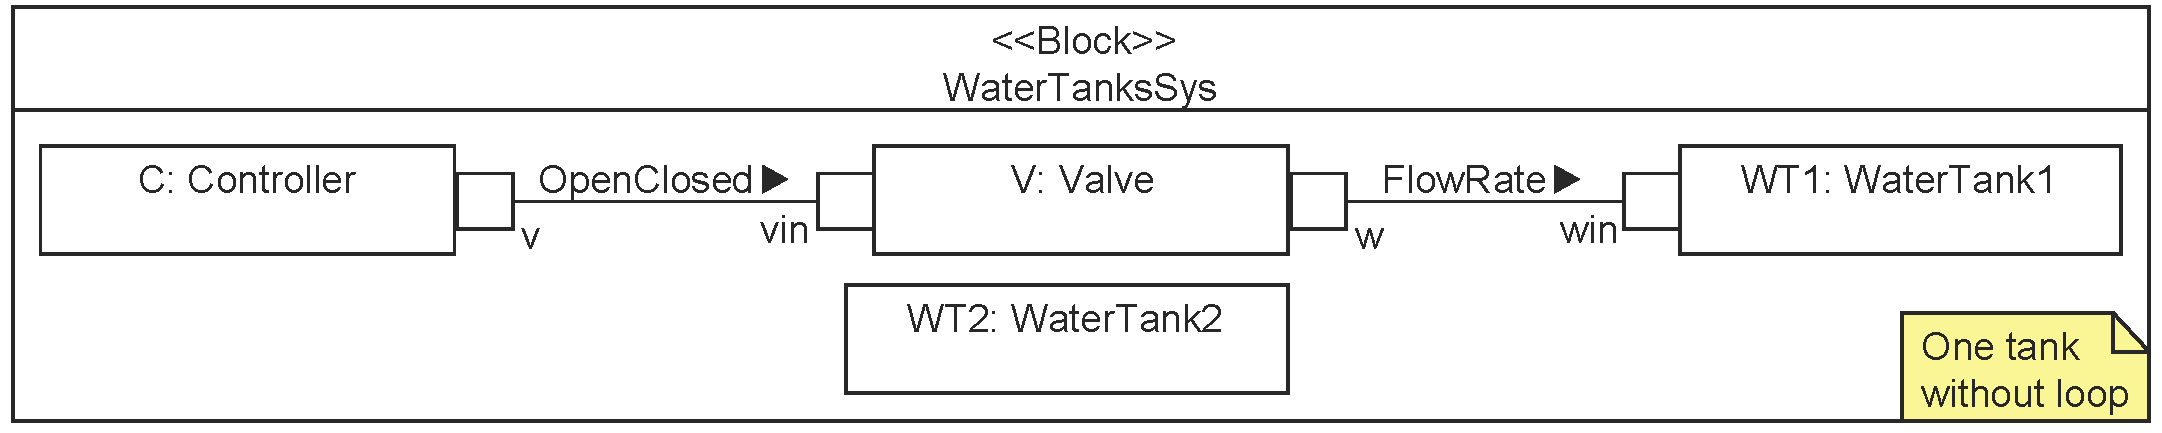
\includegraphics[width=4.5in,height=1.0in]{fig/3/CD1.png}
			\label{cd1}}
		\hfil
		\subfigure[情形2]{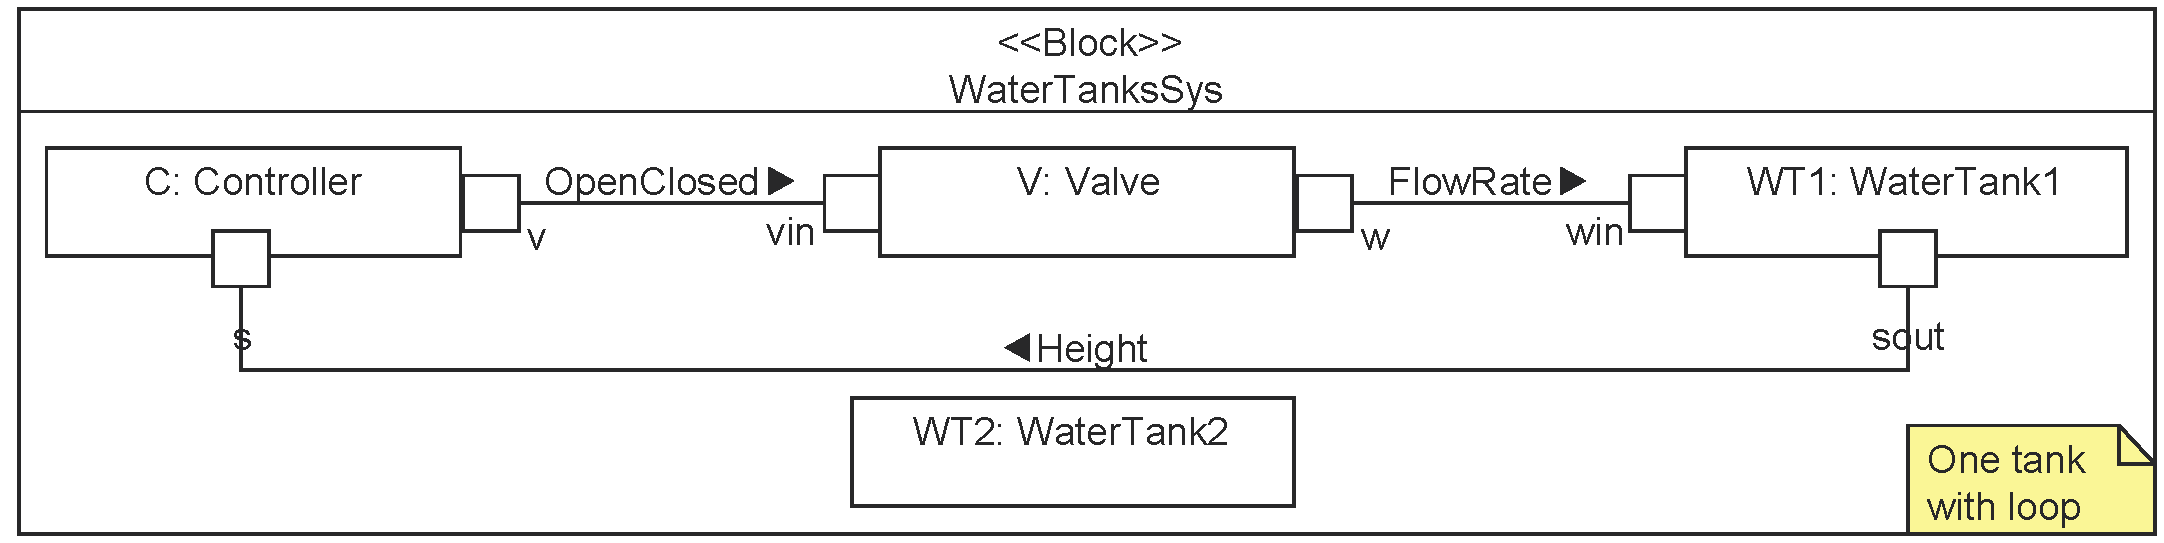
\includegraphics[width=4.5in,height=1.0in]{fig/3/CD2.png}
			\label{cd2}}
		\hfil
		\subfigure[情形3]{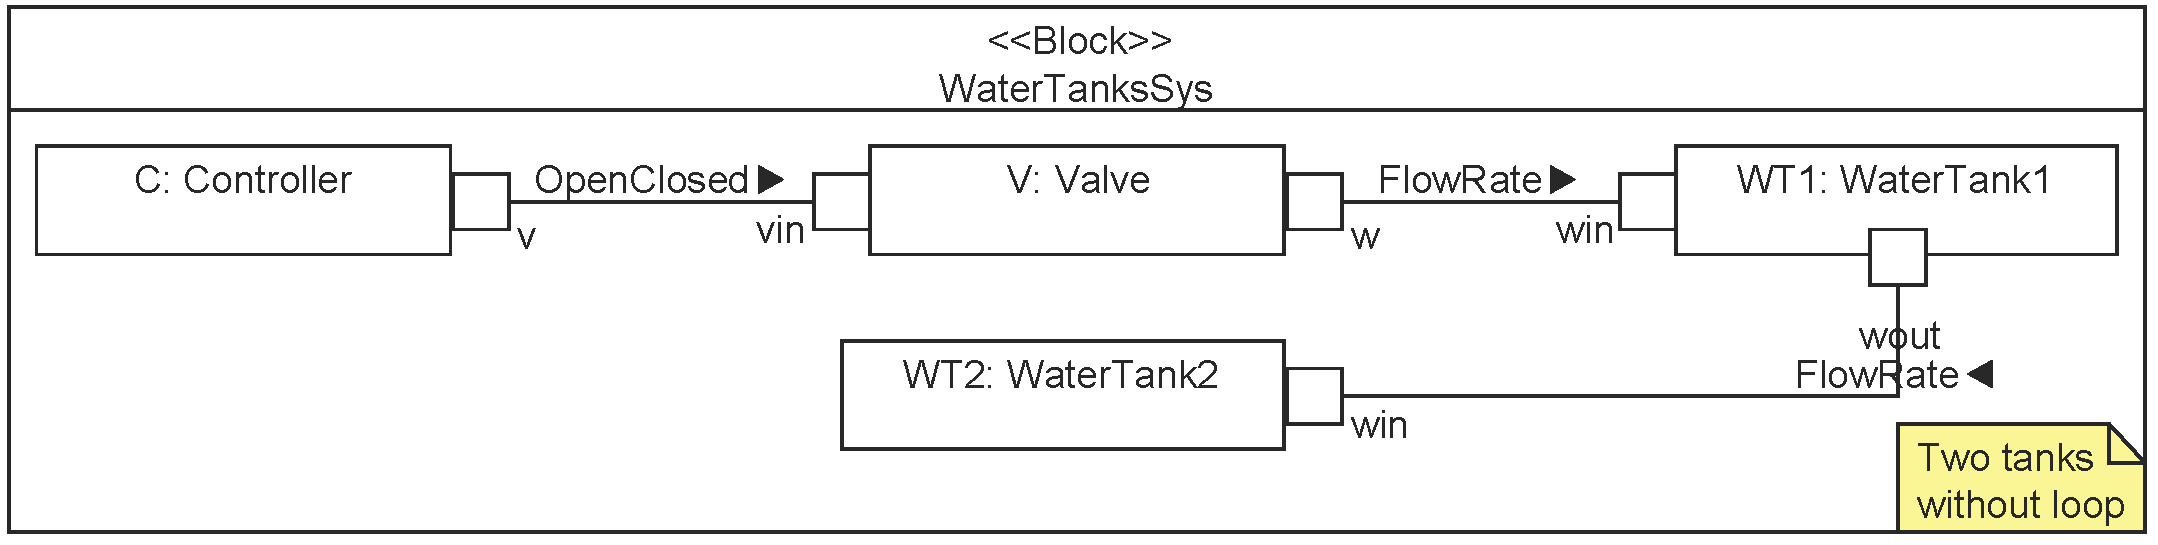
\includegraphics[width=4.5in,height=1.0in]{fig/3/CD3.png}
			\label{cd3}}
	\caption{水箱系统的SysML IBD}
	\label{cd}
	}
\end{figure}
在本小节我们用SysML BDD图描述了系统组件的结构,并用SysML的IBD图描述了各个组件之间的连接。在下一个小节,我们基于FMI标准用FMU来实现每一个系统组件,并将SysML IBD中描述的关联关系用一个FMU之间的接口配置文件进行表示。
\subsection{基于FMI的连接关系配置} 
\label{sec:case}
图\ref{fmu-con}描述的是水箱系统中的FMU组件及各个FMU之间的连接。根据图\ref{cd}给定的SysML IBD,我们也得到了三种FMU的情形。第一种情形如图\ref{fmu-con1}所示,系统中有三个FMU组件:$Controller$, $Valve$ 和$WaterTank1$和两个接口$v \_ vin$及$w \_ win$。 $Controller$ 和 $Valve$由$v \_ vin$接口连接; $Valve$ 和 $WaterTank1$ 由 $w \_ win$接口连接。第二种情形如图 \ref{fmu-con2}所示,其中在第一种情形上添加了$WaterTank1$ 和$Controller$的接口$sout \_ s$,表示控制器信号的发送受到水箱$WaterTank1$的水位影响。 图\ref{fmu-con3}是第三种情形,在第一种情形上添加了另一个水箱$WaterTank2$, 水箱$WaterTank1$ 和$WaterTank2$由接口$w \_ out$连接。 
\begin{figure}[htbp]
\centering{
		\subfigure[情形1]{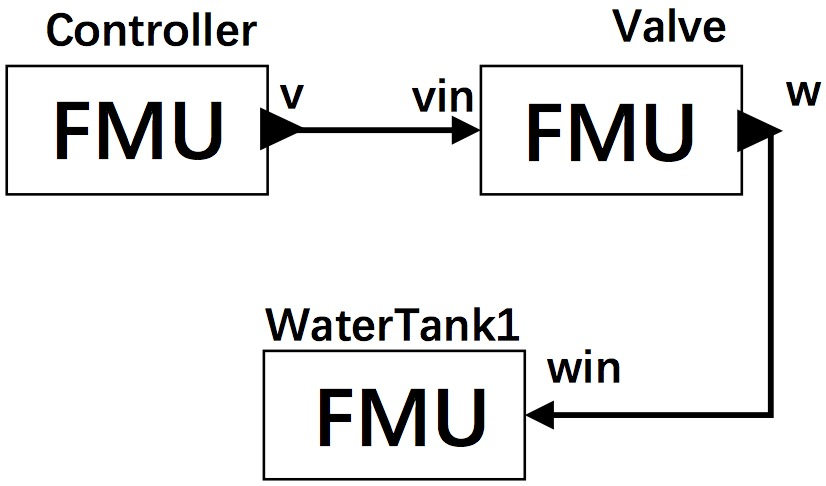
\includegraphics[width=1.5in,height=0.9in]{fig/3/fmuc1.png}
			\label{fmu-con1}}
		\hfil
		\subfigure[情形2]{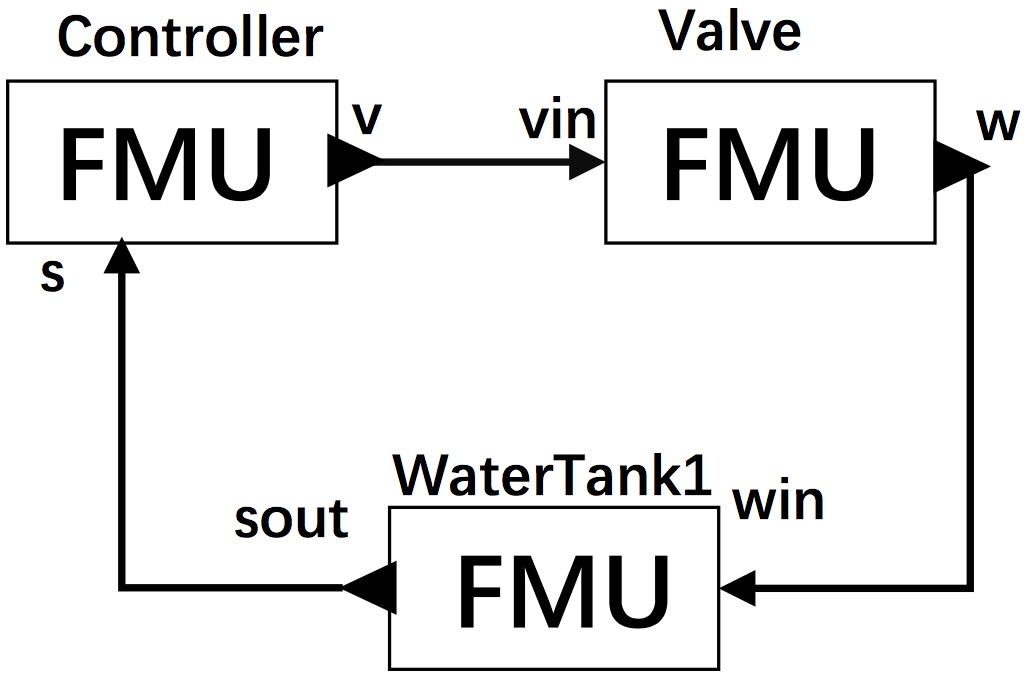
\includegraphics[width=1.5in,height=0.9in]{fig/3/fmuc2.png}
			\label{fmu-con2}}
		\hfil
		\subfigure[情形3]{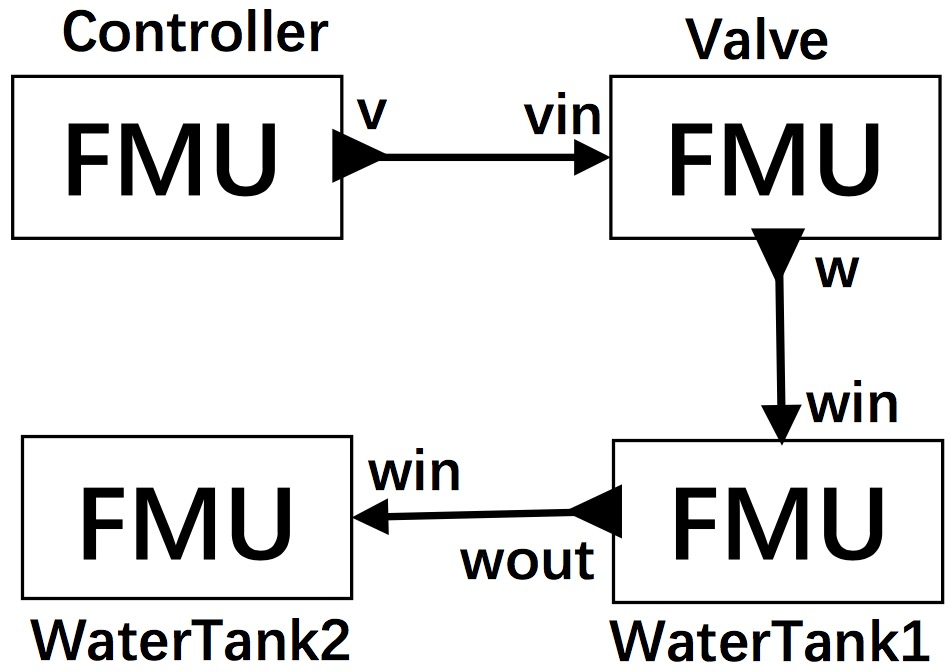
\includegraphics[width=1.5in,height=0.9in]{fig/3/fmuc3.png}
			\label{fmu-con3}}
	\caption{水箱系统中FMU的三种连接情形}
	\label{fmu-con}
	}
\end{figure}

在本小节我们设计了FMU及FMU之间的连接,我们只需要添加一个协同仿真的主算法就可以在协同仿真引擎当中对整个异构系统进行协同仿真并得到仿真迹。但是,在进行仿真之前,我们要保证各个FMU之间协同行为的正确性,因此,我们在下一个小节基于时间自动机理论对系统的协同行为进行验证,这也是我们本文的主要贡献点之一。
\subsection{协同行为的验证分析} 
\label{sec:mauppaal}
在本小节我们基于时间自动机理论对水箱系统中组件之间的协同行为的正确性进行验证。首先我们根据小节\ref{sec:encode}中提出的映射规则,将水箱系统中的FMU用时间自动机进行形式化描述,并取小节\ref{sec:ma}中建模的一个主算法(在此,采用可回滚算法作为主算法,其他算法的验证分析与该算法类似,在此不做描述),FMU之间的接口配置文件我们用时间自动机之间的信道进行描述。由此,我们得到了一个由主算法、FMU的时间自动机模型及由配置文件转化得到的信道组成的时间自动机网络。图\ref{tk-arch1}为上述小节中情形1的时间自动机网络模型。

\begin{figure}[htbp]
\centering{
		\subfigure[FMU\_controller 的时间自动机模型]{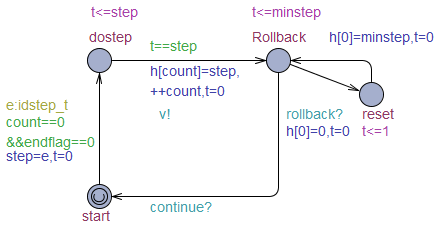
\includegraphics[width=1.6in,height=1.0in]{fig/3/2signal_controller.png}
			\label{tk_controller}}
		\hfil
		\subfigure[FMU\_valve 的时间自动机模型]{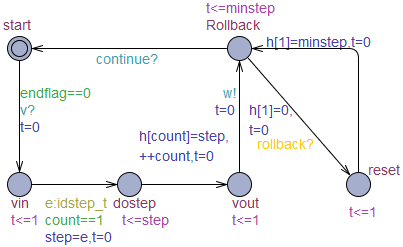
\includegraphics[width=1.6in,height=1.0in]{fig/3/2signal_v.png}
			\label{tk_v}}
			
	    \subfigure[FMU\_WaterTank1 的时间自动机模型]{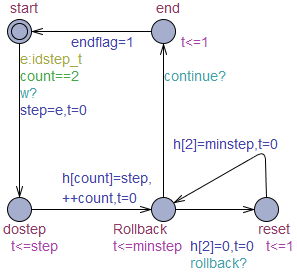
\includegraphics[width=1.5in,height=1.2in]{fig/3/2signal_wt1.png}
			\label{tk_wt1}}
		\hfil
		 \subfigure[可回滚主算法的时间自动机模型]{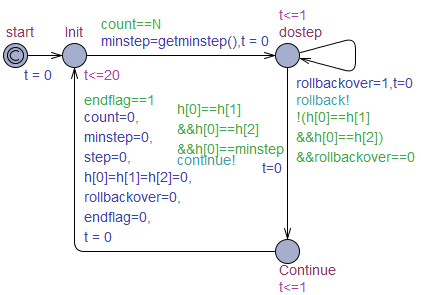
\includegraphics[width=1.7in,height=1.2in]{fig/3/2signal_master.png}
			\label{tk_ma}}		
	\caption{情形1的时间自动机网络: $controller$ $\vert\vert$ $valve$ $\vert\vert$ $WaterTank1$ $\vert\vert$ $MA$.}
	\label{tk-arch1}
	}
\end{figure}

\begin{figure}[htbp]
\centering{
		\subfigure[部分迹]{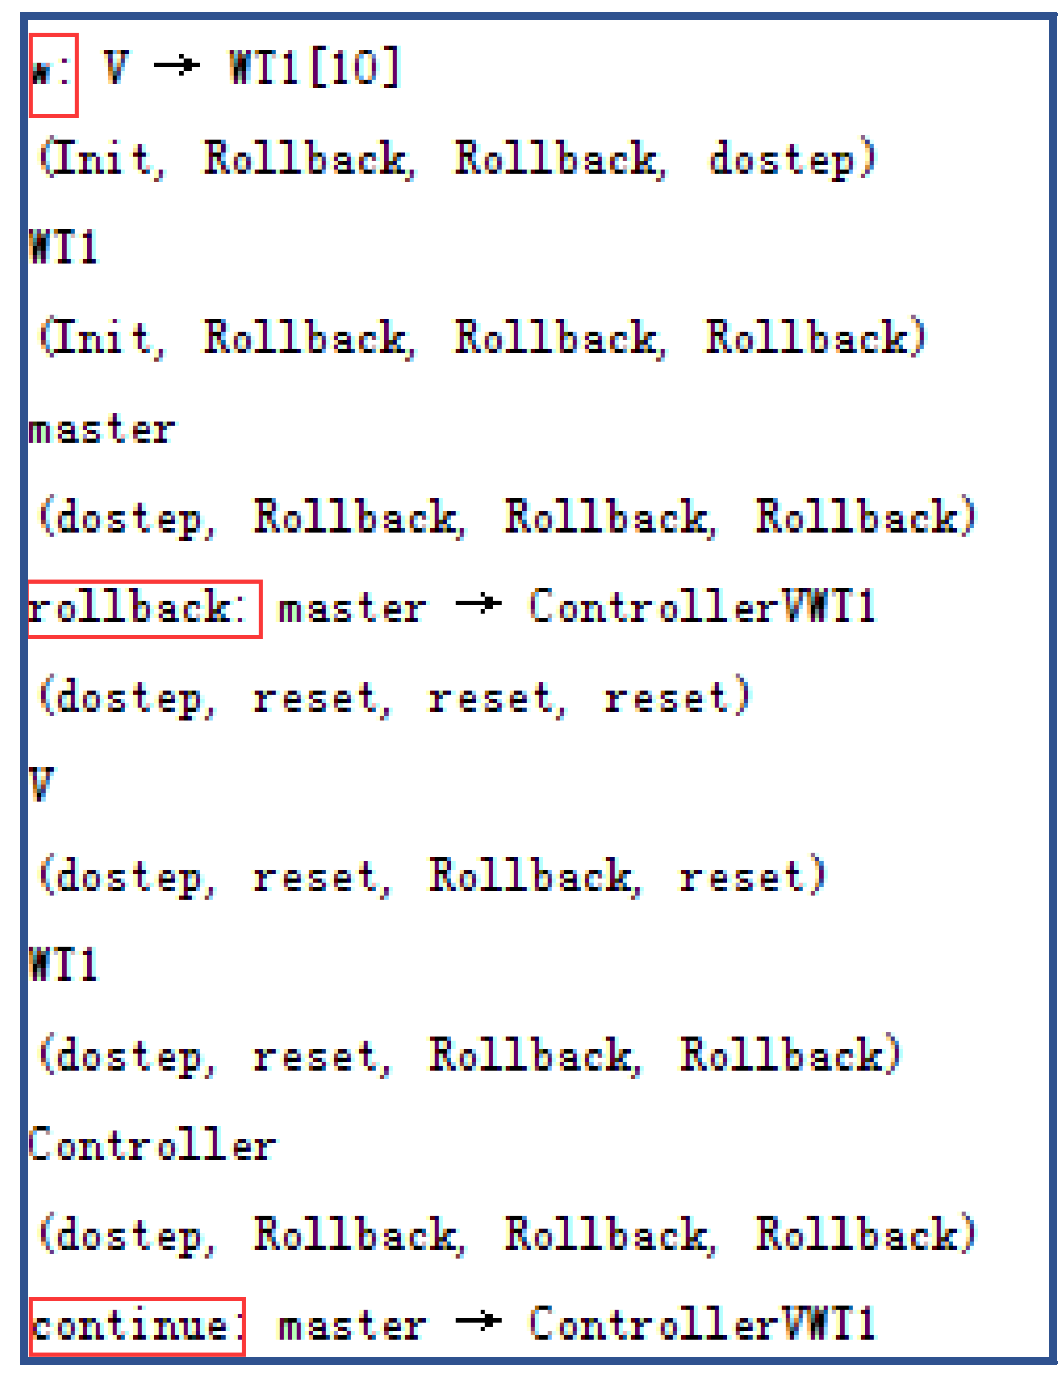
\includegraphics[width=1.6in,height=2.0in]{fig/3/trs.png}
			\label{trs}}
		\hfil
		\subfigure[执行序列图]{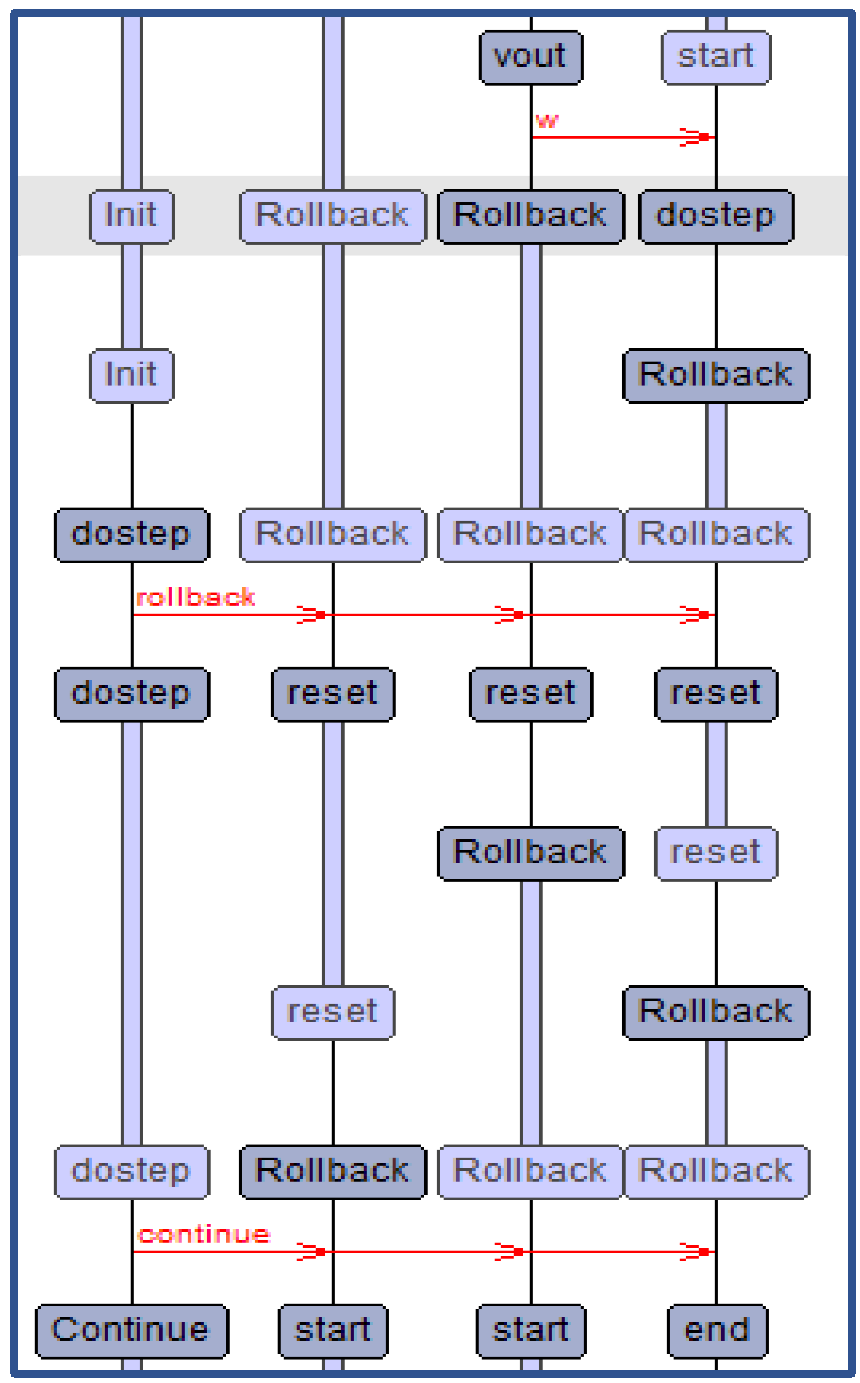
\includegraphics[width=1.6in,height=2.0in]{fig/3/seq.png}
			\label{seq}}
	\caption{协同过程在UPPAAL中的执行序列。}
	\label{trs-seq}
	}
\end{figure}

图\ref{tk_controller}, \ref{tk_v}, \ref{tk_wt1}分别是$controller$, $valve$ 和 $WaterTank1$的时间自动机模型。这些自动机都有四个主要的位置:$start$, $dostep$, $Rollback$和$reset$。图\ref{tk_controller}是 $controller$的时间自动机模型,它首先通过信道 $v$与$valve$的时间自动机模型进行交互并到达$Rollback$状态,然后等待主算法的信号,直到它收到了来自主算法的$continue$信号再与其他的FMU进行数据交互并到达$start$状态;否则,它收到$rollback$信号,并回到$Rollback$状态。$valve$和$WaterTank1$的时间自动机中位置和迁移与 $controller$类似。图\ref{tk_ma} 是主算法的时间自动机模型,首先主算法先进性参数初始化,然后根据条件来判断发出  $continue$信号或是$rollback$信号。

图\ref{trs-seq}是协同过程在UPPAAL中的执行片段,我们可以看到 $valve$ 首先发送了信号$w$ 来与 $WaterTank1$进行数据交换,然后,$WaterTank1$ 到达了 $dostep$ 状态,之后主算法广播  $rollback$信号导致FMU到达$reset$状态,最后主算法发送$continue$ 信号使得所有的FMU到达 $start$状态并开始下一步仿真。通过对执行序列的分析,我们发现模型可以正确仿真。

为了比较小节\ref{sec:case}中描述的三种情形的协同行为,我们同时用时间自动机形式化描述了其他两种情形。对于第二种情形,我们在第一种情形基础上添加了$controller$ 和 $WaterTank1$之间的信道$s$如图\ref{tk-arch2}所示;对于第三种情形我们建模了$WaterTank2$的模型并添加了信道$w2$ 如图Fig.\ref{arc3}所示。其他的模型与第一种情形中的模型类似,我们在此只给出了新增加的或有改动的模型。接下来我们将对这三种情形进行验证。
\begin{figure}[htbp]
\centering{
		\subfigure[TA for FMU\_controller]{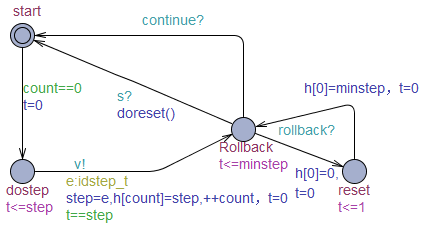
\includegraphics[width=1.8in,height=1.2in]{fig/3/2signal_cycle_controller.png}
			\label{tk2_controller}}
		\hfil
		\subfigure[TA for FMU\_WaterTank1]{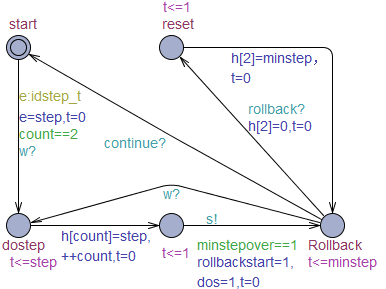
\includegraphics[width=1.5in,height=1.2in]{fig/3/2signal_cycle_wt1.png}
			\label{tk2_v}}		
	\caption{TA for connection case 2.}
	\label{tk-arch2}
	}
\end{figure}
\begin{figure}[htbp]
	\centering	{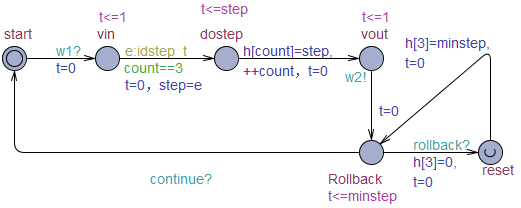
\includegraphics[width=3.5in,height=1.2in]{fig/3/4signal_wt2.png}}
	\caption{TA for FMU\_WaterTank2 of connection case 3.}\label{arc3}
\end{figure}

我们对每一种情形都验证了以下属性:
\begin{itemize}
\item
$E\langle\rangle~WT1.Rollback$和 $E\langle\rangle~master.Continue$ 为可达性验证,它表示$WaterTank1$将到达$Rollback$状态 且主算法会到达 $Continue$状态。
\item
$master.start -> master.Continue$为活性验证,它表示一旦主算法开始,它最早会到达 $Continue$状态.
\item 
$A[]~not~deadlock$为死锁的验证,它用来验证系统有无死锁。
\end{itemize}

验证结果如表\ref{rs}所示,我们发现情形1和情形3的验证属性都满足,它表示该情形的协同是正确的。然而情形2的可达性和活性不满足,是由于在该模型中出现了环路依赖,我们需要消除该环路依赖再进行下一步的仿真,在本文中我们只关注协同行为的验证,对于如何消除环路依赖在接下来的工作中我们会做进一步研究。 
\begin{table}
\caption{三种情形的验证结果}
\centering
\begin{tabular}{c c c} 
        \hline  
        情形 & 验证属性 & 结果\\
        \hline
        \multirow{2}{2.0cm}{情形1}  
                & $E\langle\rangle~WT1.Rollback$ & True\\ 
                & $E\langle\rangle~master.Continue$ & True\\ 
                & $master.start -> master.Continue$ & True\\ 
                & $A[]~not~deadlock$ & True\\   
        \hline 
        \multirow{2}{2.0cm}{情形2}  
                & $E\langle\rangle~WT1.Rollback$ & True\\ 
                & $E\langle\rangle~master.Continue$ & False\\ 
                & $master.start -> master.Continue$ & False\\ 
                & $A[]~not~deadlock$ & True\\   
        \hline 
        \multirow{2}{2.0cm}{情形3}  
                & $E\langle\rangle~WT1.Rollback$ & True\\ 
                & $E\langle\rangle~master.Continue$ & True\\ 
                & $master.start -> master.Continue$ & True\\ 
                & $A[]~not~deadlock$ & True\\   
        \hline 
\end{tabular} 
\label{rs}
\end{table}

\section{本章小结}
在本小节我们提出了一种新的方法来验证异构系统协同行为的正确性,我们首先用SysML建模语言建模了整个系统的架构,然后基于FMI标准对整个架构进行实现。之后提出了一种映射规则将FMU用时间自动机进行了形式化描述,最后基于时间自动机理论对整个系统的协同行为的正确性进行了验证。经过本小节的验证,我们可以得到通过验证的基于FMI标准的模型,该模型可以在协同仿真引擎中直接仿真并得到仿真迹,在下一个小节,我们将提出一种高效的统计模型检测方法,针对某些验证属性对协同仿真的迹进行定量的评估。
\chapter{基于分布式统计模型检测的异构系统验证分析}
\label{ch4}

%\section{基于FMI的协同仿真}
%\section{验证属性设计}
\section{基于抽象和学习的分布式统计模型检测}
\section{异构系统验证分析}

\section{本章小结}

\chapter{工具实现}
\label{ch5}

\section{异构系统验证分析工具(Co-SMC)介绍}
在本文我们提出了一种面向异构系统的验证分析方法,该方法基于协同仿真和统计模型检测,实现对异构系统行为的验证、分析。为了对该方法提供支持,我们设计、开发了异构系统验证分析工具,该工具主要由协同仿真、统计模型检测器及统计分析器三部分组成。在协同仿真器模块中,用户可以输入要进行协同仿真的多个FMU模型,然后设置仿真步长和多个FMU模型之间的参数对应关系,最后,可以从4种协同仿真算法中选择适当的协同仿真算法,对系统模型进行协同仿真并产生协同仿真的迹。统计模型检测器模块以协同仿真器产生的迹为输入,然后设置需要验证的属性,最后选择适合的统计模型检测算法进行定量的验证分析。用户可以在统计分析器模块对协同仿真器产生的迹或是统计模型检测器产生的验证结果进行统计分析,并绘制出饼状图、折线图等可视化的图形,有利于对模型的各种行为进行更加直观的分析。接下来我们对Co-SMC工具的各个部分进行详细的描述。
\begin{figure}[htbp]
	\centering
	{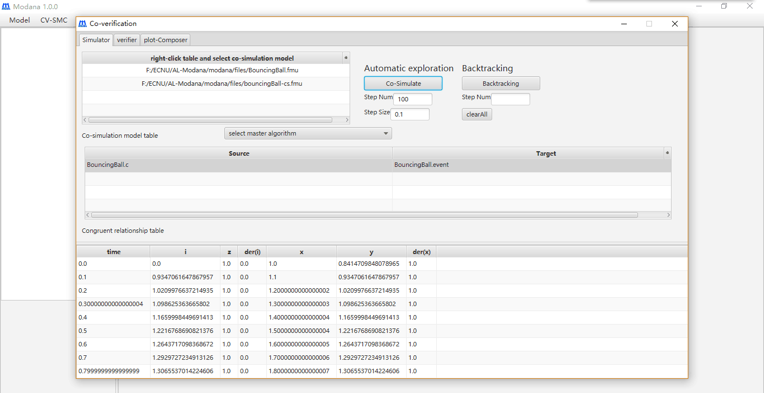
\includegraphics[width=4.0in]{fig/5/tool1.png}}
	%\vspace{0.10in}
	\caption{Co-SMC协同仿真器}\label{tool-1}
\end{figure}
\begin{figure}[htbp]
	\centering
	{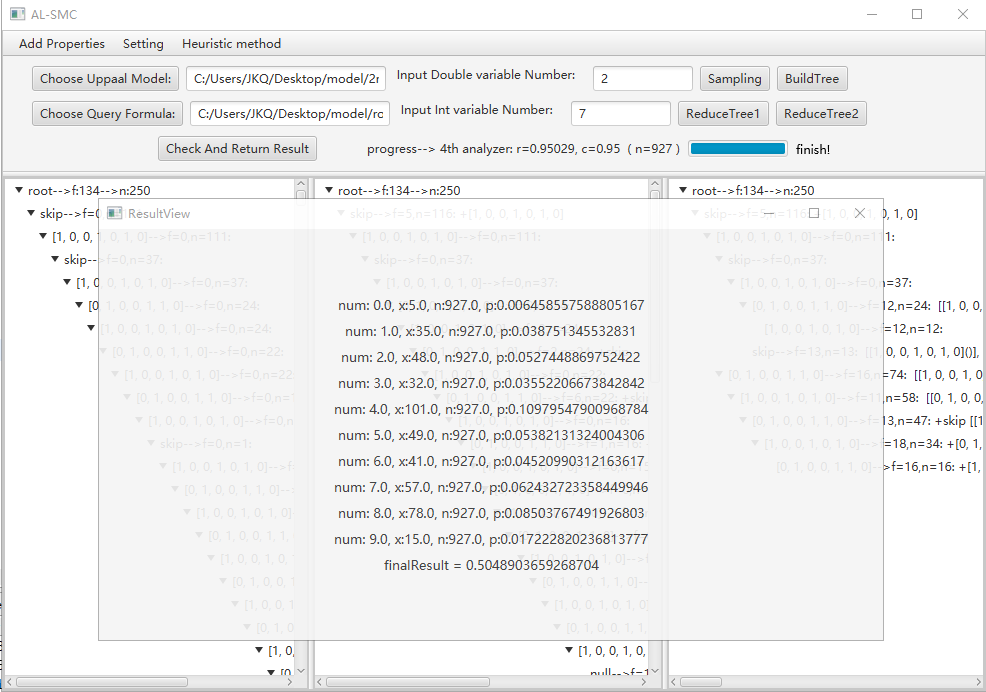
\includegraphics[width=4.0in]{fig/5/tool2.png}}
	%\vspace{0.10in}
	\caption{Co-SMC统计模型检测器}\label{tool-2}
\end{figure}
\begin{figure}[htbp]
	\centering
	{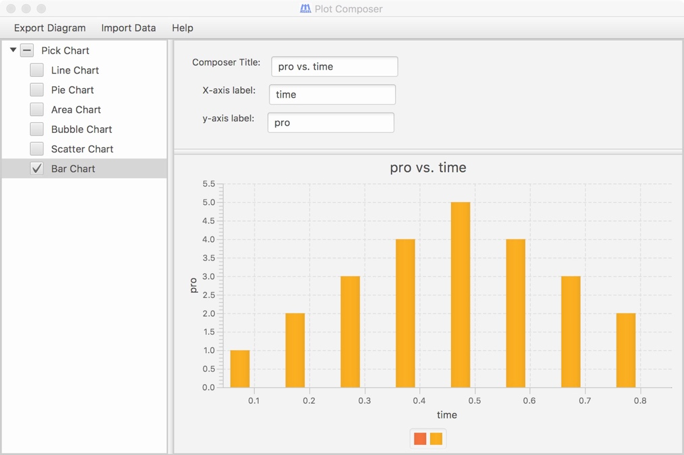
\includegraphics[width=4.0in]{fig/5/tool3.png}}
	%\vspace{0.10in}
	\caption{Co-SMC协同仿真器}\label{tool-3}
\end{figure}
图\ref{tool-1}是Co-SMC工具的协同仿真器,该工具主要包括
\section{Co-SMC程序实现}


\section{本章小结}

\chapter{案例分析与实验评估}
\label{ch6}
在本小节,我们使用两个案例(智能温控系统和机器人路径规划系统)来展示本文提出的方法的有效性。首先,我们使用SysML建模语言对这案例进行建模并根据基于FMI标准进行实现以得到基于FMI标准的仿真模型,然后我们使用章节3提出的方法对系统行为的正确性进行验证,之后将验证通过的模型进行协同仿真并将得到仿真迹用章节4提出的方法进行评估分析得到最终的评估结果。由于在章节3中我们已经使用了水箱的对整个方法进行了详细的描述,因此在本章节的案例中我们不对章节3涉及的过程做过多的描述,而是重点关注模型通过统计模型检测算法验证之后得到的评估结果及章节4提出的经过改进的算法的准确度及效率问题。
\section{案例一:智能温控系统}
智能温控系统\cite{•}在当今社会能源节约问题上起到十分重要的作用。该系统主要包含五个部分:\emph{房间温度,控制器,室外温度,加热器及用户}。控制器根据用户的行为及室内温度来控制加热器的开关,室内温度又受到室外温度、加热器及用户行为的影响。该系统的主要目的是评估某种控制策略下房间温度的舒适度及整个系统的能耗。
\subsection{系统建模与设计}

\subsection{系统验证分析}
本实验的分布式环境为五台处理器为英特尔(TM) i7-4790 (八核,主频3.6G赫兹)组成的集群。为了评估系统的行为和算法的性能,我们验证了以下三个验证属性如表 \ref{tb:property}所示。
\begin{table}[t]
	\caption{智能温控系统的验证属性}
	\label{tb:property}
	\centering
	\begin{tabular}{c c c c}
		\hline
		序号 &  $(\delta,c)$ & 验证属性 & 验证结果 \\
		\hline
		$\phi_1$ & $(0.05,0.99)$  & $P_{=?}(F^{\leq48}~energy \geq 210)$ & 0.1778 \\ 
		$\phi_2$ & $(0.01,0.99)$  & $P_{=?}(F^{\leq48}~discomfort \geq 15)$ & 0.4861\\
		$\phi_3$ & $(0.02,0.9)$ & 
		\tabincell{c}{$P_{=?}(F^{\leq48}~ discomfort \leq 15$ \\ $\wedge~energy \geq 170)$} & 0.4535 \\
		\hline
	\end{tabular}
\end{table}
我们采用贝叶斯区间估计算法对上属三条验证属性进行评估分析以得到的验证结果。下面我们对表\ref{tb:property}的验证属性及验证结果进行分析:(1)$\phi_1$用来评估在48小时内能耗超过210的概率大小,我们得到的验证结果为0.1778,表示在48小时内系统能耗超过210的可能性比较小;(2)$\phi_1$用来评估48小时内,系统的不舒适度大于15的概率,得到的验证结果为0.4861;(3)$\phi_3$用来评估在48小时内,系统的不舒适度小于15且能耗大于170的概率,得到的验证结果为0.4535。由此,可以发现本文提出的技术方法可以有效的评估异构系统的行为。

\subsection{算法评估分析}
为了评估章节4提出的算法效率,在本小节我们针对以上的三个验证属性,从产生的迹的数量,验证所需要的时间及验证误差三个方面对比了多种统计模型检测算法:贝叶斯区间估计算法(BIE)、分布式的贝叶斯区间估计算法(DBIE)、基于抽象和学习的分布式统计模型检测算法(DAL-SMC)、经过优化的基于抽象和学习的分布式统计模型检测算法(DAL-SMC opt)、分布式的APMC\cite{•}算法(DAPMC),算法对比结果如图\ref{rs_sb}所示。
\begin{figure*}[htbp]
\centering{
		\subfigure[产生的迹的数量]{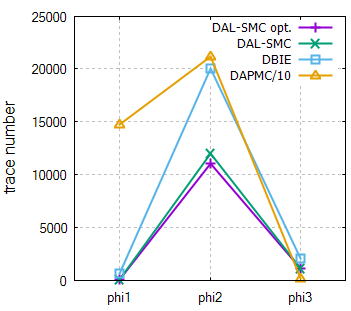
\includegraphics[width=1.5in,height=1.3in]{fig/4/sb-trace.png}
			\label{trace_sb}}
		\hfil
		\subfigure[验证时间]{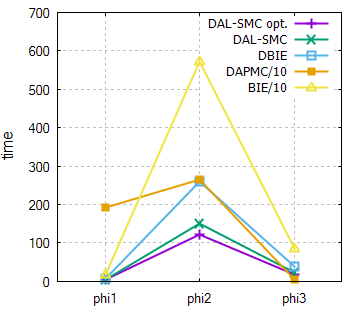
\includegraphics[width=1.5in,height=1.3in]{fig/4/sb-time.png}
			\label{time_sb}}
		\hfil
		\subfigure[验证误差]{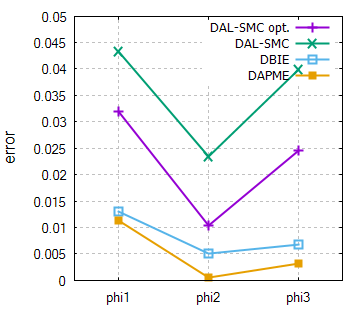
\includegraphics[width=1.5in,height=1.3in]{fig/4/sb-error.png}
			\label{error_sb}}
	\caption{智能温控系统案例算法对比}
	\label{rs_sb}
	}
\end{figure*}

图\ref{trace_sb}是算法产生的迹的数量对比,我们可以发现对于验证属性$\phi_2$,DAPMC将消耗200000条迹,然而DBIE只需要20000条迹。 DAL-SMC和 DAL-SMC opt.需要更少量的迹(大约10000条)。 算法的验证时间的对比如图 \ref{time_sb}所示,对于验证属性$\phi_2$,BIE需要6000秒,但分布式的BIE只需要大约250秒,DAL-SMC和DAL-SMC opt.需要更少的时间。图\ref{error_sb} 是算法的验证误差分析,对于验证属性$\phi1$,分布式BIE和DAPMC的误差大约为 0.013,DAL-SMC和DAL-SMC的验证误差大约为0.045和0.032。更详细的实验数据如表\ref{ta-rs}所示。 

\section{案例二:机器人路径规划系统}
在近些年来,机器人路径规划问题引起了学术界越来越多的人的关注。机器人路径规划问题的主要目标是要避免机器人与障碍物发生碰撞并最终到达目的地。本案例在经典的机器人路径规划的基础上加上能耗,即机器人在移动过程中会消耗能量且在不同的时刻消耗的能量也可能存在区别。本案例主要包含机器人及障碍物两个部分,最终我们需要评估机器人产生的能耗及机器人发生碰撞的概率大小。
\subsection{系统建模与设计}

\subsection{系统验证分析}
\begin{table}[t]
	\caption{机器人路径规划的验证属性}
	\label{tb:robot}
	\centering
	\begin{tabular}{c c c c}
		\hline
		~序号~ & $(\delta,c)$ & 验证属性 & 验证结果 \\
		\hline
		$\phi_4$ & $(0.01,0.99)$ & $P_{=?}(F^{\leq100}~robot.collision)$ & 0.2675 \\ 
		$\phi_5$ & $(0.05,0.99)$ & $P_{=?}(F^{\leq100}~energy \geq 500)$ & 0.5211 \\
		$\phi_6$ & $(0.02,0.9)$ & 
		\tabincell{c}{$P_{=?}(F^{\leq100}~robot.collision$ \\ $\wedge~energy \geq 500)$} & 0.5296\\
		\hline
	\end{tabular}
\end{table}

我们也采用贝叶斯区间估计算法对机器人路径规划的三条验证属性进行评估分析以得到验证结果。下面我们对表\ref{tb:robot}的验证属性及验证结果进行分析:(1)$\phi_4$用来评估在10小时内机器人与障碍物发生碰撞的概率大小,我们得到的验证结果为0.2675,表示在10小时内机器人与障碍物发生碰撞的可能性比较小;(2)$\phi_5$用来评估10小时内机器人消耗的能量大于500的概率大小,得到的验证结果为0.5211;(3)$\phi_6$用来评估在48小时内,10小时内机器人消耗的能量大于500的概率且不发生碰撞的概率大小,得到的验证结果为0.5296。由此,该案例也可有效说明本文提出的技术方法可以有效的评估异构系统的行为。

\subsection{算法评估分析}
通过用多种算法对机器人路径规划案例进行评估分析,得到的算法对比结果如图 \ref{rs_ro}所示:
\begin{figure*}[htbp]

\centering{
		\subfigure[产生的迹的数量]{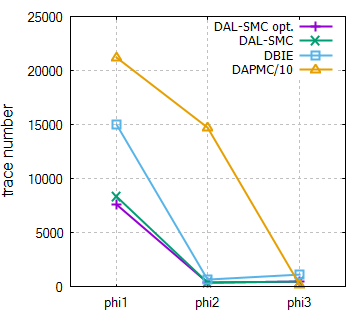
\includegraphics[width=1.5in,height=1.3in]{fig/4/ro-trace.png}
			\label{trace_ro}}
		\hfil
		\subfigure[验证时间]{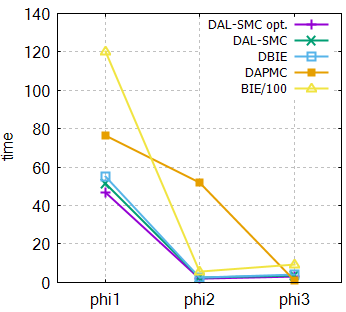
\includegraphics[width=1.5in,height=1.3in]{fig/4/ro-time.png}
			\label{time_ro}}
		\hfil
		\subfigure[验证误差]{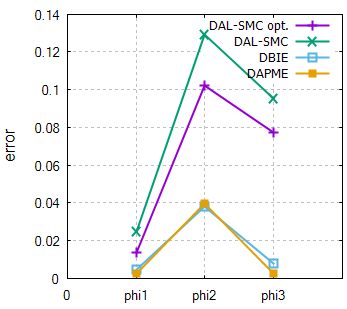
\includegraphics[width=1.5in,height=1.3in]{fig/4/ro-error.png}
			\label{error_ro}}
	\caption{机器人路径规划案例算法对比}
	\label{rs_ro}
	}
\end{figure*}

表\ref{ta-rs}给出了上述两个案例的算法对比的详细数据,下面我们针对验证属性 $\phi_2$来对算法的性能对比总结如下:
(i)DAPMC的验证需要产生最多的仿真迹,相对于DAPMC,DBIE需要的迹的数量就少很多。此外,DAL-SMC相对于DBIE又将仿真迹减少了大约一半。因此,针对产生仿真迹的数量来说,DAL-SMC是最高效的算法。

(ii)对于验证而言,产生仿真迹的过程消耗了主要的验证时间。在分布式算法之中, DAPMC消耗时间最多,DAL-SMC得益于产生较少的仿真迹而相对DBIE消耗的时间较少 。在本实验中,我们使用40个核来实现分布式算法,我们发现经典BIE算法消耗的时间大约是分布式BIE算法的25倍,由此可以说明分布式技术在提高统计模型检测算法效率上是十分有效的。

(iii)DAPMC和DBIE的验证误差较小,DAL-SMC的验证误差相对于DAPMC和DBIE较大一些。此外, 我们发现DAL-SMC opt.的误差小于DAL-SMC的验证误差,说明我们提出的参数优化方法是有效的。

总的来说,DAL-SMC opt.算法得益于分布式技术和抽象与学习技术,在验证过程中需要产生最少的仿真迹和消耗最少的验证时间,此外,由于使用了章节4提出的参数优化方法,也使得将该算法的误差控制在了一个较小的范围之内。

\begin{table*}
\caption{实验结果}
\centering
\begin{tabular}{c c c c c c} 
        \hline  
        算法 & 验证属性 & 迹的数量 & 验证时间 & 验证误差\\
        \hline
        \multirow{6}{1.5cm}{DAPMC}  
                & $\phi1(0.05,0.99)$ &  147000&  1934.31&  0.0113\\ 
                & $\phi2(0.01,0.99)$ &  \textbf{211932} &  \textbf{2649.15} &  \textbf{0.0005}\\ 
                & $\phi3(0.02,0.9)$ &  1950&     38.05& 0.0032\\ 
                & $\phi4(0.01,0.99)$ &  211930&  76.282 &  0.0024\\ 
                & $\phi5(0.05,0.99)$ &  147550&  52.206&  0.0399\\ 
                & $\phi6(0.02,0.9)$ &  1850&     1.159& 0.0026\\     
        \hline 
        \multirow{6}{1.5cm}{DBIE}  
                & $\phi1(0.05,0.99)$ &  600&  7.895&  0.0131\\ 
                & $\phi2(0.01,0.99)$ &  \textbf{20000}&  \textbf{259.275} &  \textbf{0.0051} \\ 
                & $\phi3(0.02,0.9)$ &  2100& 38.057& 0.0068\\ 
                & $\phi4(0.01,0.99)$ & 15000&  55.281 &  0.0049\\ 
                & $\phi5(0.05,0.99)$ &  702&  2.483&  0.0382\\ 
                & $\phi6(0.02,0.9)$ &  1120& 4.226& 0.0078\\      
        \hline 
        \multirow{6}{1.5cm}{DAL-SMC}  
                & $\phi1(0.05,0.99)$ &  103&  5.685&  0.0433\\ 
                & $\phi2(0.01,0.99)$ &  \textbf{12000}&  \textbf{151.785} &  \textbf{0.0235} \\ 
                & $\phi3(0.02,0.9)$ &  1137& 22.841& 0.0399\\ 
                & $\phi4(0.01,0.99)$ &  8318&  41.68 &  0.0246\\ 
                & $\phi5(0.05,0.99)$ &  384&  2.32&  0.1295\\ 
                & $\phi6(0.02,0.9)$ &  520& 3.601& \ 0.0751\\      
        \hline 
         \multirow{6}{1.5cm}{DAL-SMC opt.}  
                & $\phi1(0.05,0.99)$ &  95.79&  4.65&  0.0319\\ 
                & $\phi2(0.01,0.99)$ &  \textbf{11040}&  \textbf{121.425} &  \textbf{0.0103}\\ 
                & $\phi3(0.02,0.9)$ &  1091& 18.73& 0.0246\\ 
                & $\phi4(0.01,0.99)$ &  7569&  36.512 &  0.0138\\ 
                & $\phi5(0.05,0.99)$ &  349&  1.81&  0.102\\ 
                & $\phi6(0.02,0.9)$ &  494& 3.171& 0.0575\\     
        \hline 
         \multirow{6}{1.5cm}{BIE}  
                & $\phi1(0.05,0.99)$ &  590&  175.44&  0.0121\\ 
                & $\phi2(0.01,0.99)$ &  \textbf{19586}&  \textbf{5730.67} &  \textbf{0.0047} \\ 
                & $\phi3(0.02,0.9)$ &  2040& 845.73& 0.0063\\ 
                & $\phi4(0.01,0.99)$ & 15400&  1202.467 &  0.0044\\ 
                & $\phi5(0.05,0.99)$ &  762&  55.221&  0.0352\\ 
                & $\phi6(0.02,0.9)$ &  1150& 91.98& 0.0069\\      
        \hline 
\end{tabular} 
\label{ta-rs}
\end{table*}

\section{本章小结}
本文使用两个案例来说明本文提出的方法的可行性,首先对案例进行了建模和设计,然后重点在系统的验证分析小节中展示了本方法在对异构系统进行验证分析时的有效性,并在算法评估分析小节结合两个案例,在多个方面对比了多种算法的性能,从而展示了我们本文提出的基于抽象和学习的分布式统计模型检测算法的高效性和准确性。

\chapter{总结与展望}
\label{ch7}

%\appendix

\chapter{附录}
\vspace{-1cm}





%\begin{thebibliography}{zz}

\bibitem{built_env}
Hans-Arno Jacobsen, Randy H. Katz, Hartmut Schmeck, Christoph Goebel. Smart Buildings and Smart Grids[J]. Dagstuhl Reports, 2015, 5(2): 128-175.

\bibitem{smartbuilding}
张永坚, 周培祥, 高鹤. 智能建筑技术[M]. 中国水利水电出版社, 2007.

\bibitem{control_scheme}
Yao Jianguo, Giuseppe Tommaso Costanzo, Zhu Guchuan, Wen Bin. Power Admission Control With Predictive Thermal Management in Smart Buildings[J]. IEEE Transactions on Industrial Electronics, 2015, 62(4): 2642-2650.

\bibitem{thermal_model}
Jérôme Henri Kämpf, Darren Robinson. A simplified thermal model to support analysis of urban resource flows[J]. Energy and Buildings, 2007, 39(4): 445–453.

\bibitem{strategy_compare}
Domenico Gorni, María del Mar Castilla, José Domingo Álvarez, Antonio Visioli .A Comparison between Temperature Modeling Strategies in Smart Buildings[C]. Emerging Technologies \& Factory Automation(ETFA), 2015: 1-4.

\bibitem{performance_analysis}
Nathan Mendes, Gustavo H.C. Oliveira and Humberto X. de Araújo. Building Thermal Performance Analysis by Using matlab/simulink[C]. International Building Performance Simulation Association(IBPSA), 2001: 473-480.

\bibitem{energy1}
David A, Du Dehui, Larsen K, Mikucionis M, Skou A. An evaluation framework for energy aware buildings using statistical model checking[J]. SCIENCE CHINA Information Sciences, 2012, 55(12): 2694-2707.

\bibitem{energy2}
Chen Xiaohong, Gu Fan, Chen Mingsong, Du Dehui, Liu Jing, Sun Haiying. Evaluating Energy Consumption for Cyber-Physical Energy System: an Environment Ontology-Based Approach[C]. International Computer Software and Applications Conference, 2015: 5-14.

\bibitem{realtime}
Bouyer P, Fahrenberg U, Larsen K, Markey N. Quantitative analysis of real-time systems using priced timed automata[J]. Communications of the ACM (CACM), 2011, 54(9): 78-87.

\bibitem{uncertainty}
Chen Xiaoming, Li Xin, Sheldon X.-D. Tan. From Robust Chip to Smart Building: CAD Algorithms and Methodologies for Uncertainty Analysis of Building Performance[C]. International Conference on Computer-Aided Design(ICCAD), 2015: 457-464.

\bibitem{eval}
Du Dehui, Chen Mingsong, Liu Xiao, Yang Yun. A novel quantitative evaluation approach for software project schedules using statistical model checking[C]. International Conference on Software Engineering(ICSE), 2014: 476-479.

\bibitem{variation1}
Chen Mingsong, Yue Daian, Qin Xiaoke, Fu Xin, Mishra P. Variation-aware evaluation of MPSoC task allocation and scheduling strategies using statistical model checking[C]. Design, Automation, and Test in Europe(DATE), 2015: 199-204.

\bibitem{variation2}
Huang Saijie, Chen Mingsong, Liu Xiao, Du Dehui, Chen Xiaohong. Variation-Aware Resource Allocation Evaluation for Cloud Workflows using Statistical Model Checking[C]. International Conference on Big Data and Cloud Computing (BDCloud), 2014: 201-208.

\bibitem{pta1}
David A, Larsen K, Legay A, Mikucionis M, Poulsen D, Vliet J, Wang Zheng. Statistical Model Checking for Networks of Priced Timed Automata[C]. Formal Modeling and Analysis of Timed Systems(FORMATS), 2011: 80-96.

\bibitem{optim1}
Meysam Razmara, Guna R. Bharati, Mahdi Shahbakhti, Sumit Paudyal, Rush D. Robinett. Bidirectional Optimal Operation of Smart Building-to-Grid Systems. American Control Conference(ACC), 2015: 288-293.

\bibitem{optim2}
Zhao Hengyang, Daniel Quach, Wang Shujuan, Wang Hai, Chen Hai-Bao, Li Xin, Sheldon X.-D. Tan. Learning Based Compact Thermal Modeling for Energy-Efficient Smart Building Management[C]. International Conference on Computer-Aided Design(ICCAD), 2015: 450-456.

\bibitem{optim3}
Samuel Idowu, Saguna, Christer Åhlund, Olov Schelén. Forecasting Heat Load for Smart District Heating Systems: A Machine Learning Approach[C]. SmartGridComm, 2014: 554-559.

\bibitem{optim4}
Md. Sumon Shahriar, M. Sabbir Rahman. Urban Sensing and Smart Home Energy Optimisations: A Machine Learning Approach[C]. Internet of Things towards Applications(IoT-App), 2015: 19-22.

\bibitem{optim5}
Sakari Stenudd. A Model for Using Machine Learning in Smart Environments[C]. Grid and Pervasive Computing Workshops(GPC), 2011: 24-33.

\bibitem{ta1}
Alur R, Dill D. A theory of timed automata[J]. Theoretical Computer Science, 1994, 126(2): 183-235.

\bibitem{ta2}
Bengtsson J, Wang Yi: Timed Automata: Semantics, Algorithms and Tools[C]. Lectures on Concurrency and Petri Nets, 2003: 87-124.

\bibitem{pta2}
Behrmann G, Larsen K, Rasmussen J. Priced Timed Automata: Algorithms and Applications[C]. Formal Methods for Components and Objects, 2004: 162-182.

\bibitem{pta3}
Bulychev P, David A, Larsen K, Mikucionis M, Poulsen D, Legay A, Wang Zheng. UPPAAL-SMC: Statistical Model Checking for Priced Timed Automata[C]. Quantitative Aspects of Programming Languages and Systems, 2012: 1-16.

\bibitem{uppaal1}
Behrmann G, David A, Larsen K. A Tutorial on Uppaal[C]. Formal Methods for the Design of Real-Time Systems, 2004: 200-236.

\bibitem{model_checking}
Edmund M. Clarke, Orna Grumberg, Doron A. Peled. Model checking[M]. MIT Press, 2001.

\bibitem{smc1}
Axel Legay, Benoît Delahaye, Saddek Bensalem. Statistical Model Checking: An Overview[C]. Runtime Verification(RV), 2010: 122-135.

\bibitem{smc2}
Ananda Basu, Saddek Bensalem, Marius Bozga, Benoît Caillaud, Benoît Delahaye, Axel Legay. Statistical Abstraction and Model-Checking of Large Heterogeneous Systems[C]. Formal Techniques for Networked and Distributed Systems/Formal Methods for Open Object-Based Distributed Systems(FMOODS/FORTE), 2010: 32-46.

\bibitem{uppaal2}
UPPAAL. http://www.it.uu.se/research/group/darts/uppaal/about.shtml.

\bibitem{uppaal3}
Bengtsson J, Larsen K, Larsson F, Pettersson P, Wang Yi. UPPAAL - a Tool Suite for Automatic Verification of Real-Time Systems[C]. Hybrid Systems, 1995: 232-243.

\bibitem{smc3}
David A, Du Dehui, Larsen K, Legay A, Mikucionis M, Poulsen D, Sedwards S. Statistical Model Checking for Stochastic Hybrid Systems[J]. Hybrid Systems and Biology(HSB), 2012: 122-136.

\bibitem{smc4}
David A, Larsen K, Legay A, Mikucionis M, Wang Zheng. Time for Statistical Model Checking of Real-Time Systems[C]. Computer Aided Verification(CAV), 2011: 349-355.

\bibitem{thermal1}
Thermal System. http://lpsa.swarthmore.edu/Systems/Thermal/SysThermalIntro.html.

\bibitem{thermal2}
Deng Kun, Barooah P, Mehta P, Meyn S. Building Thermal Model Reduction via Aggregation of States[C]. American Control Conference, 2010: 5118-5123.

\bibitem{machine_learning1}
Machine learning. Wikipedia: https://en.wikipedia.org/wiki/Machine\_learning.

\bibitem{machine_learning2}
Stuart J. Russell, Peter Norvig. Artificial Intelligence - A Modern Approach (3. internat. ed.)[M]. Pearson Education, 2010.

\bibitem{ann}
I.A. Basheer, M. Hajmeer. Artificial neural networks: fundamentals, computing, design, and application[J]. Journal of Microbiological Methods, 2000, 43: 3–31.

\bibitem{nn}
Raúl Rojas. Neural Networks - A Systematic Introduction[M]. Springer, 1996.



\bibitem{cps1}
尹玲, 陈小红 ,刘静. 信息物理融合系统的时间需求一致性分析[J]. 软件学报, 2014, 25(2): 400-418.



\end{thebibliography}


{\fangsong
	\chapter*{致\qquad 谢}\vskip 2mm
	\vspace{-1cm}
	\large{

		在此论文完成之际,我首先要感谢我的导师杜德慧副教授。她严肃的科学态度,严谨的治学精神,精益求精的工作作风,深深地感染和激励着我。从课题的选择到项目的最终完成,杜老师都始终给予我细心的指导和不懈的支持。三年多来,杜老师不仅在学业上给我以精心指导,同时还在思想、生活上给我以无微不至的关怀,在此谨向杜老师致以诚挚的谢意和崇高的敬意。
		
		感谢在研究生学习期间给我诸多教诲和帮助的软件学院的各位老师和同学、以及和我一起生活两年半的室友,你们的执着、勤奋、以及对生活的态度,值得我学习。“君子和而不同”,我们正是如此!愿我们以后的人生都可以充实、快乐!
		
		最后感谢我的家人,谢谢你们在我成长道路上支持、鼓励我,让我独立地选择自己的人生道路;同时谢谢我的女朋友,在学习、生活中对我的帮助和鼓励!

	}
	
	\vspace{0.2cm}
	
	\vspace{0.2cm} \hspace{9.8cm}  
	姜~~凯强
	
	\hspace{9cm}  二零一八年五月
}
\chapter*{\large 攻读硕士学位期间发表论文、参与科研和获得荣誉情况}
\vskip 2mm
\vspace{-1cm}
\renewcommand{\labelenumi}{[\arabic{enumi}]}
{\heiti $\blacksquare$ 已完成学术论文}\vskip 3mm
\begin{enumerate}
	\item Cheng B, Wang X, Liu J, et al. Modana: An Integrated Framework for Modeling and Analysis of Energy-Aware CPSs[C]//Computer Software and Applications Conference (COMPSAC), 2015 IEEE 39th Annual. IEEE, 2015, 2: 127-136. (一作)
	\item 杜德慧, 程贝, 刘静. 面向安全攸关系统中小概率事件的统计模型检测[J]. 软件学报, 2015(2):305-320. (二作,导师一作)
	\item Cheng B, Du D. Towards a Stochastic Occurrence-Based Modeling Approach for Stochastic CPSs[C]//2014 Theoretical Aspects of Software Engineering Conference (TASE). IEEE, 2014: 162-169.(一作)
	
\end{enumerate}


{\heiti $\blacksquare$ 参与的科研课题}\vskip 3mm
\begin{enumerate}
	
	\item
	信息物理融合系统的随机行为建模与验证方法研究(国家自然科学基金面上项目, 61472140)
	
	\item
	基于统计模型检测的信息物理融合系统的验证方法研究(上海市自然科学基金项目, 14ZR1412500)
	
\end{enumerate}

{\heiti $\blacksquare$ 获得荣誉情况}\vskip 3mm
\begin{enumerate}
	
	\item
	2015年获得国家奖学金
	
	\item
	2015年获得华东师范大学优秀学生称号
	
\end{enumerate}


\begin{document}

\pagestyle{empty}

\noindent{{\zihao{4} {\large 2018} 届研究生硕士学位论文}}
\hskip 4.75cm {{\zihao{4} ~~学校代号: {\large 10269}}}\\
\hspace*{\fill} {{\zihao{4} 学号: {\large 51151500019}}}

\vskip 2cm

\begin{center}
\scalebox{1.0}{
\includegraphics[width=15cm]{fig/ecnu.eps}}
\end{center}

\vskip 3cm

\begin{center}
{\zihao{2}\bf 基于协同仿真和统计模型检测的信息物理融合系统验证分析方法}
\end{center}

\vskip 3cm {\Large
\begin{center}
\begin{tabular}{l}
院\qquad\ \ \ 系:\\
专~业~名~称:\\
研~究~方~向:\\
指~导~教~师:\\
硕士研究生:
\end{tabular}
\begin{tabular}c
~~计算机科学与软件工程学院 \\
\hline  软件工程 \\
\hline  可信软件  \\
\hline ~~杜德慧\  副教授  \\
\hline ~~姜\ 凯强\   \\
\hline
\end{tabular}
\end{center}}

\vskip 30mm

\begin{center}
{\Large 2018年5月}
\end{center}

\clearpage\ \newpage
\newpage

\pagestyle{empty}

\noindent{\large 2016 MASTER’S  DISSERTATION}
\hskip 1.4cm {\large School Code: 10269}\\
\hspace*{\fill} {\large Student Number: 51131500003}

\vskip 2cm

\begin{center}
{\Huge $\mathbb{EAST}\,\mathbb{CHINA}\,\mathbb{NORMAL}\,
\mathbb{UNIVERSITY}$}
\end{center}

\vskip 3cm

\begin{center}
{\huge \bf \scshape Statistical Model Checking Based on Abstraction and Learning}
\end{center}

\vskip 2cm {\large
\begin{center}
\begin{tabular}{l}
Department:\\
			\\
Major:\\
Research Direction:\\
Supervisor:\\
Candidate:
\end{tabular}
\begin{tabular}c
~~~School of Computer Science  \\
\hline ~~and Software Engineering  \\
\hline ~~~Software Engineering  \\
\hline ~~~Trustworthy Software  \\
\hline ~~~Associate Professor ~Dehui Du~  \\
\hline ~~~Bei~Cheng  \\
\hline
\end{tabular}
\end{center}}

\vskip 30mm

\begin{center}
{\Large May, 2016}
\end{center}

\clearpage\ \newpage
\newpage
\pagestyle{empty}
\centerline{\bf\Large 华东师范大学学位论文原创性声明}

\vskip 1cm

\normalsize \indent
郑重声明:本人呈交的学位论文《基于抽象和学习的统计模型检测研究》,是在华东师范大学攻读硕士/博士(请勾选)学位期间,在导师的指导下进行的研究工作及取得的研究成果。除文中已经注明引用的内容外,本论文不包含其他个人已经发表或撰写过的研究成果。对本文的研究做出重要贡献的个人和集体,均已在文中作了明确说明并表示谢意。
$$\\  $$

\qquad\qquad{作者签名}:$\underline{\qquad\qquad\qquad }$
\qquad \qquad\qquad \mbox {日期}:\qquad 年 \qquad  月 \qquad  日


\vskip 1cm

\centerline{\bf\Large 华东师范大学学位论文著作权使用声明}

\vskip 1cm

《基于抽象和学习的统计模型检测研究》系本人在华东师范大学攻读学位期间在导师指导下完成的硕士/博士(请勾选)学位论文,本论文的研究成果归华东师范大学所有。本人同意华东师范大学根据相关规定保留和使用此学位论文,并向主管部门和相关机构如国家图书馆、中信所和“知网”送交学位论文的印刷版和电子版;允许学位论文进入华东师范大学图书馆及数据库被查阅、借阅;同意学校将学位论文加入全国博士、硕士学位论文共建单位数据库进行检索,将学位论文的标题和摘要汇编出版,采用影印、缩印或者其它方式合理复制学位论文。

本学位论文属于(请勾选)

(  )1.经华东师范大学相关部门审查核定的“内部”或“涉密”学位论文*,
于     年    月    日解密,解密后适用上述授权。

(  )2.不保密,适用上述授权。
$$\\ $$
\qquad\qquad \mbox{导师签名}:$\underline{\qquad\qquad\qquad\qquad}$
\qquad\qquad \mbox {本人签名}:$\underline{\qquad\qquad\qquad\qquad }$

\vskip 1cm

$\rightline{ \qquad 年 \qquad  月 \qquad  日 \qquad\qquad}$

\vskip 1cm

* “涉密”学位论文应是已经华东师范大学学位评定委员会办公室或保密委员会审定过的学位论文(需附获批的《华东师范大学研究生申请学位论文“涉密”审批表》方为有效),未经上述部门审定的学位论文均为公开学位论文。此声明栏不填写的,默认为公开学位论文,均适用上述授权)。

\clearpage\ \newpage
\newpage
\pagestyle{empty}
$$\\ \\ \\ $$

\centerline{\bf\Large $\underline{\mbox{\kaishu {程贝}}}\,\,
	$硕士学位论文答辩委员会成员名单}

\vskip 10mm

\begin{center}
	{\large
		\begin{tabular}{| p{25mm}| p{30mm}| p{48mm}| p{25mm}|}\hline
			\vfill\hfill{\heiti 姓名}\hspace*{\fill} &\vfill\hfill{\heiti 职称}\hspace*{\fill} &
			\vfill\hfill{\heiti 单位}\hspace*{\fill} &\vfill\hfill {\heiti 备注} \hspace*{\fill} \\[6pt]\hline
			\vfill\hfill{\kaishu 缪淮扣}\hspace*{\fill} &\vfill\hfill{\kaishu 教授}\hspace*{\fill} &\vfill\hfill{\kaishu 上海大学}\hspace*{\fill} & \vfill\hfill {\kaishu 主席}\hspace*{\fill} \\[6pt]\hline
			\vfill\hfill{\kaishu 胡豪东}\hspace*{\fill} &\vfill\hfill{\kaishu 高级工程师}\hspace*{\fill} &\vfill\hfill{\kaishu \tabincell{c}{中航工业航空动力\\控制系统研究所} }\hspace*{\fill} & \vfill{\heiti }\\[20pt]\hline
			\vfill\hfill{\kaishu 陈铭松}\hspace*{\fill} &\vfill\hfill{\kaishu 教授}\hspace*{\fill} &\vfill\hfill{\kaishu 华东师范大学}\hspace*{\fill} & \vfill{\heiti }\\[20pt]\hline
			\vfill\hfill{\kaishu ~~~}\hspace*{\fill} &\vfill\hfill{\kaishu ~~~}\hspace*{\fill} &\vfill\hfill{\kaishu ~~~}\hspace*{\fill} & \vfill{\heiti }\\[20pt]\hline
			\vfill\hfill{\kaishu ~~~}\hspace*{\fill} &\vfill\hfill{\kaishu ~~~}\hspace*{\fill} &\vfill\hfill{\kaishu ~~~}\hspace*{\fill} & \vfill{\heiti }\\[20pt]\hline
			\vfill\hfill{\kaishu ~~~}\hspace*{\fill} &\vfill\hfill{\kaishu ~~~}\hspace*{\fill} &\vfill\hfill{\kaishu ~~~}\hspace*{\fill} & \vfill{\heiti }\\[20pt]\hline
			%              &             &              &  \vfill{\heiti }\\[20pt]\hline
		\end{tabular}
	}
\end{center}


\clearpage\ \newpage

%\newpage
\pagenumbering{roman}
\pagestyle{plain}
\vspace{-2.5cm}
\chapter*{\zihao{2}\heiti{摘~~~~要}}
%\vskip 1cm
%\vspace{-1cm}

信息物理融合系统(Cyber Physical Systems,CPS)是一种更关注计算机与物理环境交互和协作的高级嵌入式系统,自2006年此概念被提出以来,已受到了学术界与工业界的高度关注。第一,CPS应用大都安全攸关或功耗要求严苛,在保证功能的前提下,仍必须满足一定的非功能属性,如吞吐量、能耗等,因此需要验证分析以保证其可信性;第二,CPS大都是异构的混成系统,融合了连续的物理过程和离散的系统行为,且处于高度不确定的开放环境中,因此使用传统的方法(如模型检测和定理证明)难以完成验证分析。为缓解此问题,人们开始尝试使用统计算法对系统模型的仿真Trace进行分析,求得近似结果,并给出结果的误差范围,这种方法被称为统计模型检测(Statistical Model Checking,SMC)。SMC无需遍历状态空间,但当结果精度要求较高时需要产生大量Trace(多数仿真软件的Trace生成比较耗时),性能因此大大降低,本文即针对SMC的性能问题展开深入研究。

首先,对已有SMC算法的原理进行了剖析,实现了4种SMC算法,通过大量实验给出了详细的性能评估。基于实验结论,提出了一个自适应的SMC算法框架,以根据不同属性的预估概率,动态地选择合适的SMC算法。

其次,为改进自适应的SMC中贝叶斯区间估计算法的不足,提出了基于抽象和学习的SMC方法,旨在减少统计分析所需的Trace数量以提高SMC的效率。其中结合已有的抽象和学习理论(如主成分分析、随机文法推断),对随机混成自动机的仿真Trace进行了概率等价抽象和简化;并基于抽象Trace学习出概率等价的系统行为模型——前缀频率树,同时提出了树的两阶段约减算法,以有效控制树的规模,为更高效的SMC验证分析提供了良好的抽象模型。

最后,介绍了我们实现的CPS建模分析平台——Modana,基于此平台实现了本文提出的SMC改进算法,基于Modana平台建模分析了典型的CPS系统——智能温控系统;并结合3个基准测试案例,对SMC算法改进前后的性能和准确度进行了实验性评估。结果证明,本文提出的SMC改进方法正确并且有效。

\hspace{-0.5cm}
\sihao{\heiti{关键词:}} \xiaosi{信息物理融合系统;随机混成自动机;主成分分析;统计抽象;统计模型检测}

\newpage
\vspace{-1cm}
\chapter*{\zihao{-2}\heiti{ABSTRACT}}
%\vspace{-0.5cm}

Cyber Physical Systems (CPS) are advanced embedded systems concerning more the interaction and collaboration between computer and physical environment. Since 2006 when this concept was presented, they have been highlighted by both academic and industrial worlds. First, most CPS applications are safety-critical or limit demanding energy consumption; a number of non-functional requirements (e.g. throughput, energy consumption, etc) need to be met when functional ones have been guaranteed, so that they required to be checked to achieve trustworthy systems. Second, most CPS are heterogeneous hybrid systems which combine continuous physical process and discrete system behavior, and also are exposed to open environment of high uncertainty; so traditional methods (model checking and theorem proving) can hardly finish checking effectively. To mitigate this issue, statistical methods are used to analyze the traces drawn from system simulator, by which an approximate result are obtained with an error bound. This method is known as Statistical Model Checking (SMC) which does analysis without traversing the state space of systems. However, SMC with high precision usually consumes a large number of traces (generating traces is seriously time-consuming for most simulation softwares), which leads to poor performance. This paper intensely studies the performance issue of SMC.

First of all, we gives an insight into the theory of existing SMC algorithms and implement four of them for conducting large numbers of experiments of their performance in detail. Based on our conclusion, an adaptive SMC algorithm framework is presented to automatically choose appropriate SMC algorithms according to the estimated probability of properties in different cases.

Next, to overcome the shortcoming of Bayesian Interval Estimate in the adaptive SMC, we present an SMC method based on abstraction and learning, aimed at improving the efficiency of SMC via reducing the number of traces for statistical analysis. This method uses the existing related learning theories (e.g. principal components analysis and stochastic grammar inference) to abstract and simplify probabilistically equivalent traces of Stochastic Hybrid Automata. Then we learn the probabilistically equivalent system behavior model, i.e. prefix frequency tree with abstracted traces, and effectively control the size of the tree by two-phase reduction algorithms presented also in this paper. It provides a well abstract model for more efficient verification and analysis with SMC later.

Finally, we introduce Modana Platform for modeling and analysis of CPS, which is implemented by our team. Based on Modana, we further implements the improved SMC presented in this paper. And a typical CPS application - smart heating system is modeled and analyzed. Then we experimentally evaluate the performance and accuracy of both original and improved SMC algorithms with three benchmarks. It turns out that our method is correct and efficient.

%\hspace{-0.5cm}
{\sihao{\textbf{Keywords:}}} \textit{Cyber physical systems, Stochastic hybrid automata, Principal components analysis, Statistical abstraction, Statistical model checking}




































\setcounter{tocdepth}{2}
\tableofcontents

\newpage
\pagenumbering{arabic}
\pagestyle{fancy}

\CTEXsetup[format+={\zihao{3}\heiti}]{chapter}
\CTEXsetup[format+={\raggedright\zihao{4}\heiti}]{section}
\CTEXsetup[format+={\zihao{-4}\heiti}]{subsection}


\setlength{\baselineskip}{25pt}  %%正文设为25磅行间距

\chapter{绪\hskip 0.4cm 论}
\label{ch1}

\section{研究背景及意义}

信息物理融合系统(Cyber Physical System,CPS)是一种复杂的异构系统,具有以下两个特征:1)面向开放环境,存在大量不确定因素,如天气突变、信号误差、人为失误等,都需要在设计CPS 时予以考虑,以保障CPS 在未知环境下的可信性;2)除了计算机外,还结合了机械、环境、土木、电子、生物、化学、航空等诸多工程领域的模型和方法,且各领域不是简单地关联,而是深度的融合。
因此,由于CPS的不确定性、异构性及连续性,使CPS的建模分析及验证面临巨大的挑战,已有的CPS研究已经针对CPS的各个性质做了大量的工作,并相应的有了一些工具的支持,例如基于时间自动机理论的UPPAAL,基于马尔科夫模型的Prism以及对物理系统提供较好的建模仿真支持的Modelica、Simulink等等。然而,以上工作在解决CPS的建模验证及仿真问题上各有优势及不足。
本文首先提取出信息物理融合系统的信息部分(cyber part)、物理部分(physical part)以及需求约束(constraint),之后对信息部分和物理部分分别用合适领域的建模工具进行建模,同时将需求约束抽象成验证属性(property), 其次我们将针对建好的多个模型设计master算法进行协同仿真(Co-simulation),并生成协同仿真的迹(trace),最后将生成的协同仿真的迹输入到我们的验证器(checker)并使用分布式统计模型检测算法进行评估分析。本方法可以很好的结合多种建模仿真工具的的建模优势,从而更好的支持对CPS系统的建模、仿真和定量评估。 


\section{国内外研究现状}

\subsection{CPS的形式化建模}
对CPS 进行验证分析的基础是形式化建模。模型无论在系统设计还是系统分析中都处于核心地位,良好的模型可以为一个复杂的系统提供合适的抽象,并有助于理解系统行为的本质,但CPS 的内在异构性使其很难拥有一个完美的建模范式。目前常见的模型如下:
1.	Ptolemy II 是由加州大学伯克利分校的Edward A. Lee 教授团队完成,着重于解决异构系统建模、设计和仿真问题的强大工具。其基于Actor 模型,为多种不同的计算模型(Models of Computations,MoCs)提供了一种强语义,以达到在一个完整系统中融合多种MoCs 的目标。因此,Ptolemy 方法特别适用于大型的异构CPS。
2.	随机混成自动机(Stochastic Hrbrid Automata,SHA)可视作混成自动机的扩展。由于CPS 与控制论同源,而混成系统又适合于刻画一般控制系统,所以扩展的混成自动机也可用来建模CPS。在混成自动机中,常微分方程(Ordinary Differential Equation,ODE)可包含在状态中,用来表示系统停留在该状态时所进行的连续变化过程,状态之间的跳转仍然为离散行为。SHA 大体可分为两类,一类是仅仅将随机行为引入离散的状态跳转中,如Piecewise-deterministic Markov processes;另一类则更加复杂,还将随机过程引入到了连续变化中,如中提出的随机混成系统。特别的,UPPAAL-SMC 将代价时间自动机网(Network of Priced TimedAutomata,NPTA)中的时钟变化率扩展为非常数形式,其表达能力等价于第一类SHA。
3.	Petri 网是另一种常见的性能分析模型,适合描述同步并发系统,因其丰富直观的表达风格而得到广泛应用。目前Petri 网也已有针对CPS 的特点进行扩展的版本。


\subsection{分布式技术(Distributed technology)}
分布式计算技术是计算机发展过程中产生的一项科学技术,主要工作原理是通过多台计算机的分布式连接实现数据的综合处理,旨在通过多台计算机的强大的工作能力来分解复杂问题,解决一些计算难题。分布式计算技术的具体特征表现如下:首先,分布式计算能够合理分配计算内容,实现多台计算机共同工作,节约设备成本,提高工作效率。其中最核心的内容在于能够为计算程序寻找最合适的计算机来完成工作。目前,计算机领域内关于分布式计算的技术已有数百种之多,但多数并没有密切的联系,这种缺乏系统管理和统一行业规定的技术并不利于日后的广泛发展。另外,分布式计算技术主要是通过科学算法的研究,形成一种独特的计算模型,确保其超长的数据处理能力,这种发展规律导致大多数用户只单纯研究如何集结更多闲置计算机来完成实际数据的处理,并没有考虑如当某些计算机丧失处理能力后的数据归属问题。那么,就要求研究者对分布式计算技术进行更加深入、系统的研究,目前,通过虚拟网络运营机制来实现大批量数据的共同处理以及如何实现用户间数据的高速共享以初具规模。如何更大规模的集结剩余计算力量、如何科学系统的管理共享数据资源、如何更大程度的节省计算资源成本成为当今社会研究分布式计算技术的重要课题。

\subsection{协同仿真(Co-simulation)}
由于CPS包含信息和物理两个部分,并涉及各个领域,因此,对于CPS的各个部分的建模在不同的领域都有相应的工具及方法支持。如果将CPS各个部分联系在一起进行仿真分析通常有两种方法: 1)开发一个统一的CPS建模平台,将CPS的所有相关部分都在此平台建模仿真分析2)将CPS的各个部分在不同的工具中建模,使用协同仿真技术[22,23]联合CPS的各个部分进行仿真。方法一到目前为止实现起来较为复杂,所以通常采用第二种方法较多,但协同仿真技术在实际的仿真中需要消耗较多的时间,针对这一问题,我们之前提出了[24]有效的提高了协同仿真的效率。

\subsection{统计模型检测(Statistical Model Checking)}
人们利用统计知识来分析系统由来已久,SMC技术即建立在蒙特卡洛模拟、假设检验等统计方法之上,通过统计分析系统仿真运行的Trace来验证系统属性满足的情况。它最早被Sen等人提出用来验证黑盒系统\cite{sen2004statistical},即Single Sampling Plan(SSP)算法的雏形,其难点在于确定算法收敛所需的Trace总样本数量$N$以及接受原假设的阈值$C$;Younes等人在博士论文\cite{younes2005verification}中提出一种二叉搜索的算法来近似得到所需的$n$和$c$,并指出了\cite{sen2004statistical}中验证黑盒系统方法的一些错误。基于Wald的Sequential Probability Ratio Test(SPRT)\cite{wald1945sequential}原理,Younes等人还提出了基于对数的SPRT实现算法\cite{younes2005verification,younes2006statistical},用以验证系统;该方法可以最小化算法所需Trace的样本数量。SSP与SPRT用以解决定性验证问题,回答了“系统$S$满足属性$\phi '$的概率是否大于或等于某个概率阈值$\theta$”这个问题,即$S \models P_{\geq \theta} (\phi ')$。与定性算法不同,定量算法可以直接返回$S$满足$\phi '$的概率$p$,如Approximate Probabilistic Model Checking(APMC)\cite{herault2004approximate},通过计算$x/n$来计算$p$(其中$x$和$n$分别表示所需的Trace正样本数量和总数量),并通过Chernoff-Hoeffding界来限定结果的误差范围。随后,Zuliani、Clarke等人基于贝叶斯统计又提出了两个新SMC实现算法:Bayesian Hypothesis Testing(BHT)和Bayesian Interval Estimation(BIE)\cite{jha2009bayesian,zuliani2013bayesian},前者基于贝叶斯假设检验解决定性验证问题,后者基于贝叶斯区间估计解决定量评估问题。

从SSP、SPRT、APMC到BHT、BIE,SMC算法所需Trace数量逐渐减少,效率逐渐提高。为了进一步探索SMC技术,许多人将数值方法与统计方法相结合\cite{bogdoll2011partial,pavese2013automated},来进一步提升SMC效率或解决一些SMC难以应付的问题,如非确定性问题(Non-determinism)。研究SMC非确定性算法的还有Henriques等人,其博士论文讨论了如何用概率方式近似解决非确定性问题\cite{henriques2012statistical}。SMC善于验证有界(通常指时间约束,即time-bounded)的属性,因此传统模型检测中的无界“Until”属性的SMC验证方法也是研究热点之一,He、Jennings等人提出了一种将无界“Until”验证转化为有界“Until”的方法以解决此问题\cite{he2010bounded,jennings2012two}。由于SMC基于系统仿真结果,所以也不可避免地引入了仿真领域的问题,比如小概率事件在Trace中出现概率极低,使得验证过程需要产生Trace的数量过多而效率低下。Jegourel、Legay等人基于重要性取样(Importance Sampling)和重要性分割(Importance Splitting)技术提出了面向小概率属性验证的SMC算法\cite{jegourel2012cross,jegourel2013importance},大大减少了验证所需的Trace样本数量;解决类似问题还可以借助于机器学习技术,如\cite{du2015smc4rare}借助支持向量机预测事件,\cite{kumar2014efficient}借助贝叶斯推断预测事件,都可以提高SMC的效率。除此之外,SMC还有一些特殊的应用场景,如黑盒系统\cite{sen2004statistical}、异构系统\cite{basu2010statistical,vodenvcarevic2012learning},允许在系统内部结构和行为未知的条件下分析系统。

Ymer\cite{younes2005ymer}和Vesta\cite{sen2005vesta}是最早实现SMC的验证工具。Vesta采用了极易实现并行化的SSP算法的一个变种,Ymer采用的SPRT算法很快也被Younes证明同样能够被并行化。Ymer在实验中的效率高于Vesta;此外,Vesta还支持了无界“Until”的验证。目前最流行的支持SMC的验证工具则是UPPAAL-SMC\cite{bulychev2012uppaal}和Prism\cite{kwiatkowska2011prism},UPPAAL-SMC和Prism都实现了定性的SPRT算法,同时都实现了基于置信区间(Confidence Interval,CI)\cite{brown2001interval}的定量算法(文献\cite{pires2008interval}对不同版本的CI统计算法进行了对比,并根据需求的不同,给出了方法选择的建议)。UPPAAL-SMC的建模基于PTA或SHA,使用图形化建模,用户友好,对于时间和连续行为的支持较好;Prism则使用Reactive Modules Language(RML)建模,对随机(如马尔科夫链)和非确定性(如马尔科夫决策过程)模型的验证支持较好。Plasma Lab\cite{boyer2013plasma}是新出现的一款纯SMC工具,同样支持RML建模,并实现了多种SMC算法(包括重要性取样和分割等面向小概率事件的算法)。Plasma Lab允许用户以插件集成的方式为其添加新的模型输入和验证算法,如Simulink的集成。

\section{本文技术路线及主要研究内容}
信息物理融合系统是异构系统,本文针对这种异构系统的验证提出了一种解决方案,图\ref{pa-fra}为本文的技术路线图,本文的技术路线大致如下:

(1)我们通过对该系统进行分析,提取出该系统的信息部分(Cyber part)和物理部分(Physical part),除此之外我们根据自己需要验证的行为属性定义约束(Constraint)。

(2)使用SysML\cite{•} 建模语言对提取出的信息部分和物理部分进行建模,将信息系统和物理系统的组件使用SysML的BDD(SysML Block Definition Diagram )图进行建模,同时使用SysML的IBD(SysML Internal Block Diagram)图来描述系统中各个组件之间的关联。

(3)SysML只是用来建模组件内部结构和组件之间的关联,该模型不可直接进行仿真运行,因此我们将SysML BDD图建模的模型使用FMU进行实现,同时将SysML IBD图描述的系统组件关系转化为FMU之间相互依赖的接口配置文件,此时,我们只需要再设计好协同仿真的主算法(Master Algorithm)就可以进行异构系统的协同仿真。然而,在进行协同仿真之前,我们首先要保证各个FMU之间的协同是正确的,要确保FMU之间协同行为的正确性,我们需要验证主算法的正确性及各个FMU之间的连接顺序及数据交换的正确性。在本文中,我们基于时间自动机设计了一个协同行为正确性验证的验证器,我们将系统的多个FMU、协同仿真的主算法以及FMU之间的接口配置文件输入到该协同行为的验证器之中即可验证当前系统协同行为的正确性,如果验证通过则说明我们当前的模型即为正确的模型,如果验证不通过,则需要修改当前系统的协同行为,直到得到验证通过的模型之后再输入到仿真器中进行仿真。

(4)我们在进行系统的验证分析时,首先需要验证的系统模型,同时我们还需要验证的属性(Property),我们将(1)中得到的约束进行形式化描述,即可得到验证属性(该验证属性根据约束的不同可以是BLTL/ALTL/GSCL等等)。

(5)将通过第三步验证的模型(Verified Model)及第四步得到的验证属性输入到异构系统验证器(co-verification)之中进行验证分析,首先将模型输入到仿真器(Simulator)之中进行仿真或协同仿真(Co-simulation)并得到仿真迹(Traces),然后将得到的仿真迹和验证属性输入到模型验证器(Checker)之中来验证该迹是否满足某条特定的验证属性,得到结果满足为1,不满足为0,我们将该验证是否满足的结果称为观察值(Observations),多条仿真迹对于一条特定的验证属性会得到多个观察值。最后将得到的观察值输入到统计分析算法中进行统计分析,并得到评估结果。
\begin{figure}[htbp]
	\centering
	{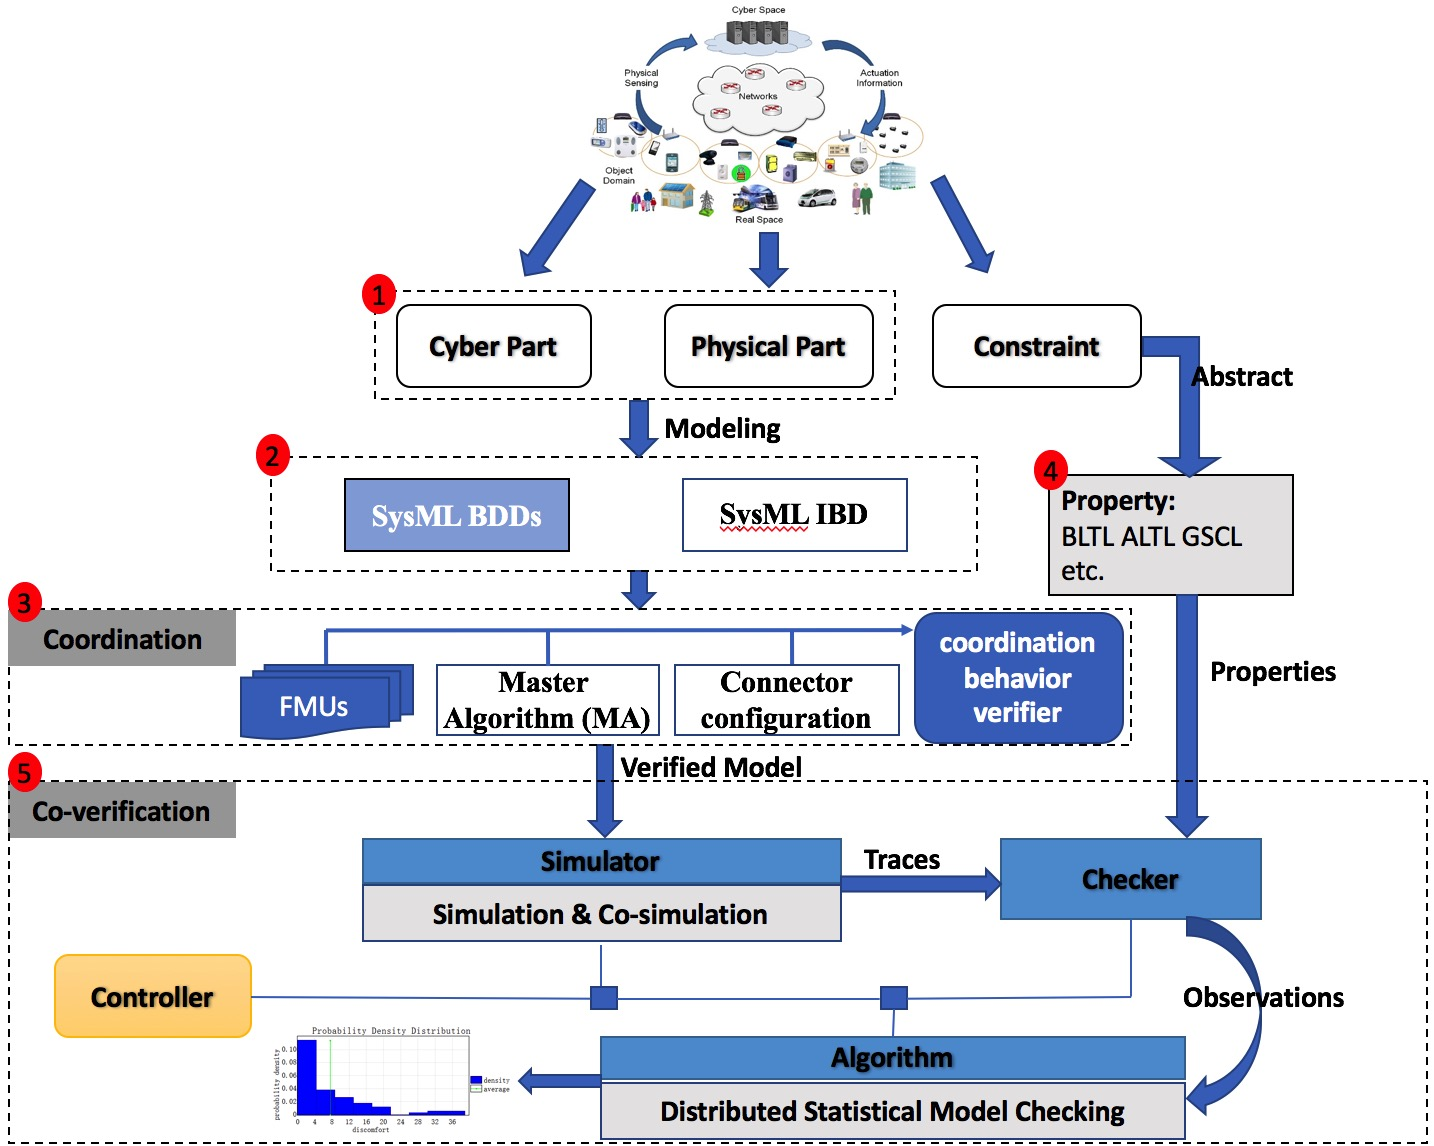
\includegraphics[width=6.0in]{fig/1/paper-framework.jpg}}
	%\vspace{0.10in}
	\caption{论文技术路线图}\label{pa-fra}
\end{figure}

\textbf{本文的具体研究内容和贡献点总结如下}:
\begin{enumerate}
	\item 使用SysML建模语言建模整个系统的架构,使用SysML的BDD图建模系统组件,使用SysML的IBD图来描述系统中各个组件的关联关系。
	\item 基于FMI标准实现SysML描述的系统模型,将SysML的BDD图建模的系统组件包装成FMU,并将各个组件的关联关系转化为FMU之间的接口配置文件。
    \item 使用时间自动机理论验证了基于FMI标准的多个组件的协同行为,使用时间自动机将协同仿真的主算法进行形式化描述,并使用UPPAAL \cite{•} 模型检测器来验证主算法的正确性;提出了一种从FMU到时间自动机的映射标准,通过此标准用时间自动机将多个FMU进行编码,并用时间自动机之间的通道(channel)来描述多个FMU之间的关联关系,最终将多个FMU及FMU之间的关联关系使用一个时间自动机网络进行了描述,将该时间自动机网络输入到UPPAAL之中进行验证从而来验证协同行为的正确性。
    \item 将验证属性用BLTL/ALTL/GSCL等形式化语言进行描述。
    \item 提出了一种基于抽象和学习的分布式统计模型检测算法,大大提高了统计模型检测的效率。
\end{enumerate}

\section{本文组织结构}
本文共分七章,组织结构如下:

第一章介绍了本文的研究背景及意义,并从四个方面阐述了该研究领域的国内外研究现状,其中包括信息物理融合系统的形式化建模、分布式技术、协同仿真及统计模型检测的研究现状。之后,给出了本文的技术路线和主要贡献点。最后,总结了论文组织结构。

第二章介绍了相关预备知识。首先给出了信息物理融合系统的主要概念,并详细讨论了我们本文关注的信息物理融合系统的异构性;之后,给出了概率有界线性时态逻辑和时间自动机的形式化描述,并给出了基于FMI标准的协同仿真通用接口。

第三章介绍了基于时间自动机理论来验证异构系统协同行为正确性的方法,首先我们给出了该方法的技术框架,之后我们详细描述了如何用时间自动机理论来验证协同仿真的主算法,以及如何验证整个异构系统的协同行为的正确性。

第四章重点阐述了如何用统计模型检测算法来对异构系统进行验证分析,也是本文的主要内容。首先,介绍了如何基于FMI标准对异构协同进行协同仿真并得到仿真迹,然后提出了一种基于抽象和学习的统计模型检测算法来提高统计模型检测的效率。最终,我们将协同仿真和该高效的统计模型检测算法进行结合,以此来对异构系统进行验证分析。

第五章主要介绍工具及程序实现。首先简单介绍了我们自己的CPS建模分析平台——Modana,之后给出了基于Modana平台的异构系统验证工具(Co-SMC工具)。最后,给出了Co-SMC工具的详细设计及程序实现。

第六章给出了两个案例,通过使用本文提出的方法对这两个案例进行建模、仿真和分析来验证本文提出方法的有效性。

第七章为总结和展望,总结了本文提出的基于分布式统计模型检测的异构系统验证方法,并讨论了其优点和不足,指出了未来要进一步进行研究的工作。
\section{本章小结}
本章首先说明了选题的背景和意义,指出了由于CPS的异构性而导致CPS系统的验证分析面临巨大挑战;接着介绍了信息物理融合系统的形式化建模、分布式技术、协同仿真及统计模型检测的研究现状;最后给出了本文的技术路线、主要贡献点和组织结构。下一章将介绍本文涉及到的预备知识及概念。

\chapter{预备知识与概念}
\label{ch2}
\section{功能模拟接口(FMI)}
CPS中各个组件之间的协同仿真可以基于FMI标准来实现,FMI标准最初是在2008年开始的MODELISAR项目中开发的,并得到大量软件公司和研究中心的支持。FMI支持模拟由异构组件组成的复杂系统,通过一个协同仿真环境将不同模型与自己的求解器耦合起来。实现了FMI标准接口的系统组件被称为FMU,我们可以基于FMI标准将模型转化为FMU,之后加入协同仿真的主算法就可以对系统进行协同仿真,其中主算法并不是FMI标准的一部分。FMI标准包含两个主要部分:
\begin{enumerate}
\item 协同仿真接口:一组用来实现对仿真器控制和完成多个FMU之间进行数据传输的C语言函数。
\item 协同仿真描述文件:用一个XML文件定义了模型的结构和主要的描述信息。主要包括模型的输入、输出信息,模型的仿真器和求解器等等。
\end{enumerate}
FMI至今已经有两个版本,即FMI1.0和FMI2.0\cite{Broman2013Determinate}。FMI1.0中有一个主要的函数是doStep,主函数可以调用该函数,使得FMI中的某个FMU进行一步的仿真。该函数的定义如下:\\
fmiStatus fmiDoStep( fmiComponent c, fmiReal currentCommunicationPoint, fmiReal communicationStepSize, fmiBoolean newStep); 

其中,$c$为主算法要调用的FMU组件,$currentCommunicationPoint$为主算法当前的仿真时间,$communicationStepSize$是主算法要FMU下一步进行仿真的步长。FMU接收到主算法的调用命令和调用步长时,将会接受或拒绝这一步长,如果接受这一步长则到进行仿真并到达一个新的状态,如果拒绝则需要重新调用。$newStep$用来表示当前的这一次仿真是一次新的调用还是拒绝之后的再次调用。

FMI2.0针对FMU1.0做了一定的扩展,主要是增加了$fmiGetFMUstate$和$fmiSetFMUstate$两个方法。这两个方法使得FMU可以对状态进行保存和恢复,从而支持了FMU状态的回滚。在后续章节,我们提出的支持回滚的主算法是基于这一扩展进行设计的。因此,扩展之后的doStep函数如下:\\
fmiStatus fmiDoStep(fmiComponent c, fmiReal currentCommunicationPoint, fmiReal communicationStepSize, fmiBoolean noSetFMUStatePriorToCurrentPoint);

其中,前三个参数跟FMU1.0里面的参数相同,只是最后一个参数的含义与FMI1.0有了本质的区别,通过设置$noSetFMUStatePriorToCurrentPoint$为true和false,主算法可以来控制FMU是否将之前一个状态的值设置给当前时间节点。
\section{功能模拟单元(FMU)}
我们在以上小节介绍了FMI标准接口,下面我们对实现了FMI标准接口的FMU给出形式化的语法和语义。
\begin{define}
\textbf{FMU 语法}

FMU的语法可以用一个八元组$F=(S,U,Y,D,s_{0},set,get,doStep)$表示,
\end{define}
\begin{itemize}
\item
$S$ 表示FMU的状态集合。
\item
$U$ 表示FMU的输入变量集合。
\item
$Y$ 表示FMU的输出变量集合。
\item
$D \subseteq U \times Y$ 表示多个FMU之间输入和输出之间的依赖关系集合。 $(u,y) \in D $表示输出变量$y$直接依赖于输入变量$u$的取值。 
\item
$s_{0} \in S$ 表示FMU的初始状态。
\item
$set : S \times U \times \mathbb{V} \rightarrow S$表示$set$函数对一个输入变量进行赋值。给定当前状态$s \in S$, 输入变量 $u \in U$及一个数值 $v \in \mathbb{V}$, 该函数将返回一个新的状态,此状态中$u$的值为$v$。
\item
$get : S \times Y \rightarrow \mathbb{V}$表示$get$函数返回某个输出变量的数值。给定一个状态 $s \in S$和一个输出变量$y \in Y$, $get(s,y)$返回$s$状态上$y$输出变量的取值。
\item
$doStep : S \times \mathbb{R}_{\geqslant{0}} \rightarrow S \times \mathbb{R}_{\geqslant{0}}$表示$doStep$函数进行了一步仿真。给定当前状态$s$和一个非负实数$h \in \mathbb{R}_{\geqslant{0}}$, $doStep(s,h)$返回一个元组$(s^{\prime},h^{\prime})$,且
\\
    当$h^{\prime} = h$时, $F$接受该步长并执行步长为$h$的仿真,并且迁移到了一个新的状态 $s^{\prime}$;
\\
    当$0 \leqslant h^{\prime} < h$时,$F$拒绝步长$h$,只执行步长为$h^{\prime}$的仿真,并且迁移到一个新的状态 $s^{\prime}$。
\end{itemize}
\begin{define}
\textbf{FMU 语义}
\end{define} 
给定一个FMU$F=(S,U,Y,D,s_{0},set,get,doStep)$,FMU的执行依赖于$doStep$函数,它的执行可以用一个时间输入序列(Timed Input Sequence, TIS)进行描述。TIS是一个有限的四元组序列$(t,s,v,v^{\prime})$, $t \in \mathbb{R}_{\geqslant{0}}$表示当前时刻,$s \in S$表示$F$的当前状态,$v$是一个输入变量,$v^{\prime} : Y \rightarrow \mathbb{V}$ 是一个输出变量。
 
TIS = $(t_{0},s_{0},v_{0},v_{0}^{\prime}), (t_{1},s_{1},v_{1},v_{1}^{\prime}),(t_{2},s_{2},v_{2},v_{2}^{\prime}), ..., (t_{i},$
$s_{i},v_{i},v_{i}^{\prime}), (t_{i+1},s_{i+1},v_{i+1},v_{i+1}^{\prime}), ...$定义如下:
\begin{itemize}
\item
$t_{0} = 0$时刻的$s_{0}$状态表示$F$处于初始状态位置。
\item
对于任意的$i \geqslant 1$, $t_{i} = t_{0} + \sum_{k = 1}^i h_{k}$。
\item
给定当前状态$s_{i}$,$set$函数用来将当前状态的输入参数设置为一个特定的数值$v$,之后$F$执行$doStep$函数并且迁移到一个新的状态$s_{i}^{\prime}$。$get$函数用来得到当前状态的所有输出参数的取值$v_{i}^{\prime}$。
\end{itemize}
\section{时间自动机(TA)}
时间自动机\cite{BehrmannDLHPYH06}是一个建模实时系统行为的经典理论模型。 在本小节中,我们给出时间自动机的形式化语法和语义。
\begin{define}
\textbf{时间自动机 语法}

时间自动机可以用一个四元组$\textit{A}=(L,l_{0},E,I)$来表示,其中:
\end{define}
\begin{itemize}
\item
$L$表示时间自动机中有限的位置集合;
\item
$l_{0} \in  L$为时间自动机的初始位置;
\item
约束集合$G(x)$可以用$g = x \bowtie c \mid g \land g$来表示,其中 $x \in X$, $c \in \mathbb{N}$且$\bowtie~\in \{<,\leqslant,\geqslant,>,=\}$。
\item
$E \subseteq L \times G(X) \times Act \times 2^X \times L$是一组边的集合, 该边包含约束和时钟,其中 $Act = Act_{i} \cup Act_{o}$。$Act_{i}$是一个输入动作的集合,$Act_{o}$是一个输出动作的集合。
\item
$I : L \rightarrow G(X)$将不变量指定给位置。
\end{itemize}
\begin{define}
\textbf{时间自动机语义} 

时间自动机$\textit{A}=(L,l_{0},E,I)$的语义可以用一个标签迁移系统$L_{\textit{A}} = (Proc,Lab,\lbrace {{\xrightarrow{\alpha}}} \mid \alpha \in Lab \rbrace)$进行描述,其中:
\end{define}
\begin{itemize}
\item 
$Proc = \lbrace(l,v) \mid (l,v) \in L \times (X \rightarrow \mathbb{R}_{\geqslant{0}})$且$v \models I(l) \rbrace$,其中状态是一个$(l,v)$元组,$l$是时间自动机中的位置且$v$是满足$I(l)$的一个时钟变量;
\item
$Lab = Act \cup \mathbb{R}_{\geqslant{0}}$ 是一个标签集合;
\item
迁移关系定义如下:

$(l,v) \xrightarrow{\alpha} (l^{\prime},v^{\prime})$,如果存在一个边 $(l \xrightarrow{g,\alpha,r} l^{\prime}) \in E$,则$v \models g$, $v^{\prime} = v[r]$且$v^{\prime} \models I(l^{\prime})$

$(l,v) \xrightarrow{d} (l,v+d)$,对于所有的$d \in  \mathbb{R}_{\geqslant{0}}$,则$v \models I(l)$且$v + d \models I(l)$
\end{itemize}
对于时间自动机$A$中某个位置$l$的可达性问题就是一个判断在迁移系统$L_{A}$中是否存在一个从初始状态$(l_{0},v_{0})$到状态$(l,v)$的路径。为了验证需要,我们定义了时间自动机的符号语义,该定义用到了一组包含时钟的执行序列集合。

对于一个特定的位置$l$和特定的时刻 $t \in X$,对于任意的$x \in X$,则$t + x \in X$。从该时刻位置开始的执行序列如下所示:

$(l,t) \xrightarrow{x_{1}} (l,t+x_{1}) \xrightarrow{x_{2}} (l,t+x_{1}+x_{2}) \xrightarrow{x_{3}} (l,t+x_{1}+x_{2}+x_{3}) \xrightarrow{x_{4}}...\xrightarrow{x_{i}}(l,t+x_{1}+x_{2}+x_{3}+...+x_{i}) \xrightarrow{x_{i+1}}...$

其中$x_{i} > 0$且无穷序列$x_{1} + x_{2} + . . .$ 对于$x$是收敛的。 
\section{系统建模语言(SysML)}
SysML是为模型驱动式软件开发(Model-Based Systems Engineering,MBSE)\cite{Dori16}而提出的一种通用的领域建模语言( Domain-Specific Language,DSL)\cite{SemerathBHSV17} ,它起源于国际系统工程委员会(INCOSE)的倡议\ cite {Pepper2015International}并于2001年1月发布 。SysML基于统一建模语言2.0(Unified Modeling Language2.0,UML2.0)\cite{Bjerkander2003Architecting}的一个子集,加入了其他一些建模元素的扩张。SysML的提出是用来统一复杂系统开发的各种建模语言和技术。SysML是一种基于UML建模语言,针对系统工程做了相应的扩展而构造出的一种建模语言。它为系统的建模和需求建模提供了新的方法。 在\cite{Bjerkander2003Architecting}中,Willard B.重点介绍了UML2.0的发展,并提出了SysML带来的新的可能性,他声称SysML的主要优点是“为系统工程师提供标准和全面的系统规范范例”。 SysML使用UML2.0中的图作为类或对象图,但是采取了新的语义来避免软件词汇表(例如,类和对象被块代替)。此外,加入新的图来简化需求的声明,并针对之后的仿真提出了一些相关的设计。块(block)是SysML的基本概念。 块是描述系统的每个模块单元的基本建模元素。 块定义了一组代表组件结构和行为的特征和操作。 这些块在BDD内以层级关系进行声明和组织。 在BDD中,块拥有自己的属性,这些属性将它们的特征和子元素定义为部件和端口。此外,块还拥有它们能够执行的一组操作。IBD则显示了各个块的端口之间的连接关系。

\section{概率有界线性时态逻辑(PBLTL)}
概率有界线性时态逻辑(Probabilistic Bounded Linear Temporal Logic,PBLTL)\cite{David2012Statistical}公式可以用来形式化的描述系统的验证属性。我们先给出有界线性时态逻辑(Bounded Linear Temporal Logic,BLTL)的语法和语义,然后再将其扩展为PBLTL。

给定一个模型$M$,设其状态变量的集合$SV$是一个有限的实数集,在$SV$上的一个布尔谓词约束为$y \sim v$形式。其中$y\in SV$,$\sim \in \lbrace \geq,\leq,=\rbrace$且$v\in \mathbb{R}$。BLTL的语法定义如下:
$$\varphi ::= y \sim v\mid\phi_{1}\wedge\phi_{2}\mid\phi_{1}\vee\phi_{2}\mid \neg \phi_{1}\mid\phi_{1}U^{\leq t}\phi_{2}
$$
其中,$\sim \in \lbrace \geq,\leq,=\rbrace$,$y\in SV$,$v\in \mathbb{Q}$,$t\in \mathbb{Q}_{\geq 0}$。

定义算子“$F$”表示最终会满足,$F^{\leq t}\phi = True U^{\leq t}\phi$,表示最终在$t$时间内存在$\phi$满足;

定义算子"$G$"算子表示始终满足,$G^{\leq t}\phi = \neg F^{\leq t}\neg \phi$,表示在$t$时间内$\phi$始终满足。

对于一条仿真迹$\sigma$,$\sigma^k$表示$\sigma$从第$k$步开始执行之后的部分。我们规定$V(\sigma,k,y)$表示迹 $\sigma$在第$k$步时状态变量$y$的值,$t_k$表示第$k$步需要的时间,$t$表示时间约束,则BLTL在迹$\sigma^k$上的语义定义如下:

\begin{define}\label{def:bltl_semantics}
(有界线性时态逻辑的语义).	
\begin{itemize}
\item $\sigma^{k}\vDash y \sim v $当且仅当$V(\sigma,i,y)\sim v$。
\item $\sigma^{k}\vDash\phi_{1}\vee\phi_{2}$当且仅当$\sigma^{k}\vDash\phi_{1}$或$\sigma^{k}\vDash\phi_{2}$。
\item $\sigma^{k}\vDash\phi_{1}\wedge\phi_{2}$当且仅当$\sigma^{k}\vDash\phi_{1}$且$\sigma^{k}\vDash\phi_{2}$。
\item $\sigma^{k}\vDash\neg\phi_{1}$当且仅当$\sigma^{k}\vDash\phi_{1}$不成立。
\item $\sigma^{k}\vDash\phi_{1}U^{t}\phi_{2}$当且仅当存在数值$i$使得

$ \Sigma_{0\leq l<i}$ $t_{k+1}\leq t$;

$ \sigma_{k+i}\models\phi_{2}$;

$\sigma_{k+j}\models\phi_{1}$,对于每个$ 0\leq j \leq i$。
\end{itemize}
\end{define}

\begin{define}\label{def:pbltl}
(概率有界线性时态逻辑).

一个PBLTL属性公式$\phi$可以表示为$P_{\geq \theta}(\phi')$,其中$\phi'$为BLTL公式,$\theta$为一个阈值(介于0和1之间)。对于定性分析的PBLTL验证属性,我们将其表示为$M \models P_{\geq \theta}(\phi)$,即来验证模型$M$满足BLTL属性$\phi'$的概率是否不小于$\theta$。对于定量分析的PBLTL验证属性公式,无需指定阈值$\theta$,可以将其表示为$M \models P_{=?}(\phi')$,即来验证模型$M$满足BLTL属性$\phi'$的概率是多少。
\end{define}


\section{本章小结}
本章首先介绍了实现异构系统各个组件之间协同运行的标准,即FMI标准和FMU的语法及语义;同时,给出了用于验证组件之间协同行为正确性的理论模型-时间自动机的语法和语义。最后,给出了描述本文的验证属性主要用到的逻辑公式PBLTL的语法和语义。下一章我们将介绍如何建模整个异构系统的架构以及如何基于时间自动机理论来验证异构系统中各个组件协同行为的正确性。

\chapter{异构系统协同行为的正确性验证}
\label{ch3}
在本章节,我们首先用SysML建模语言对整个异构系统的架构进行建模,其中用SysML的BDD图来建模系统的组件,用SysML的IBD图来建模系统中各个组件之间的关联关系。由于SysML只是用来建模系统的架构,该建模语言得到的模型不可执行。因此,我们基于FMI标准,将SysML的BDD描述的组件用FMU进行实现,将SysML的IBD图转化为FMU之间的接口配置文件。因此,我们只需要设计协同仿真主算法就可以完成异构系统基于FMI的协同仿真。然而,在我们将基于FMI的可仿真模型输入到协同仿真引擎之中进行仿真之前,我们需要确保该模型的协同行为的正确性,即要保证该模型可以正确的进行协同仿真。为了解决这个问题,我们需要进行两个方面的验证:(1)我们要验证协同仿真主算法的正确性,即算法没有出现死锁以及其他一些特性;(2)我们要验证系统之间各个组件之间关联顺序及数据交互的正确性,其中最主要的要保证多个FMU没有出现环路依赖。由于FMU的执行时基于时间的,而时间自动机在建模时间有较大的优势,且时间自动机的验证有着良好的工具支持,因此,在接下来的内容中,我们重点描述如何基于时间自动机理论来验证整个可仿真模型的协同行为的正确性。在第一小节,我们给出整个验证过程的技术框架;第二小节介绍如何对上述的第一个方面进行验证,即协同仿真的主算法的验证;在第三小节中,我们使用一个具体的案例来描述如何对上述的第二个方面进行验证,即异构系统协同行为的验证。
\section{技术框架}
\begin{figure}[htbp]
	\centering
	{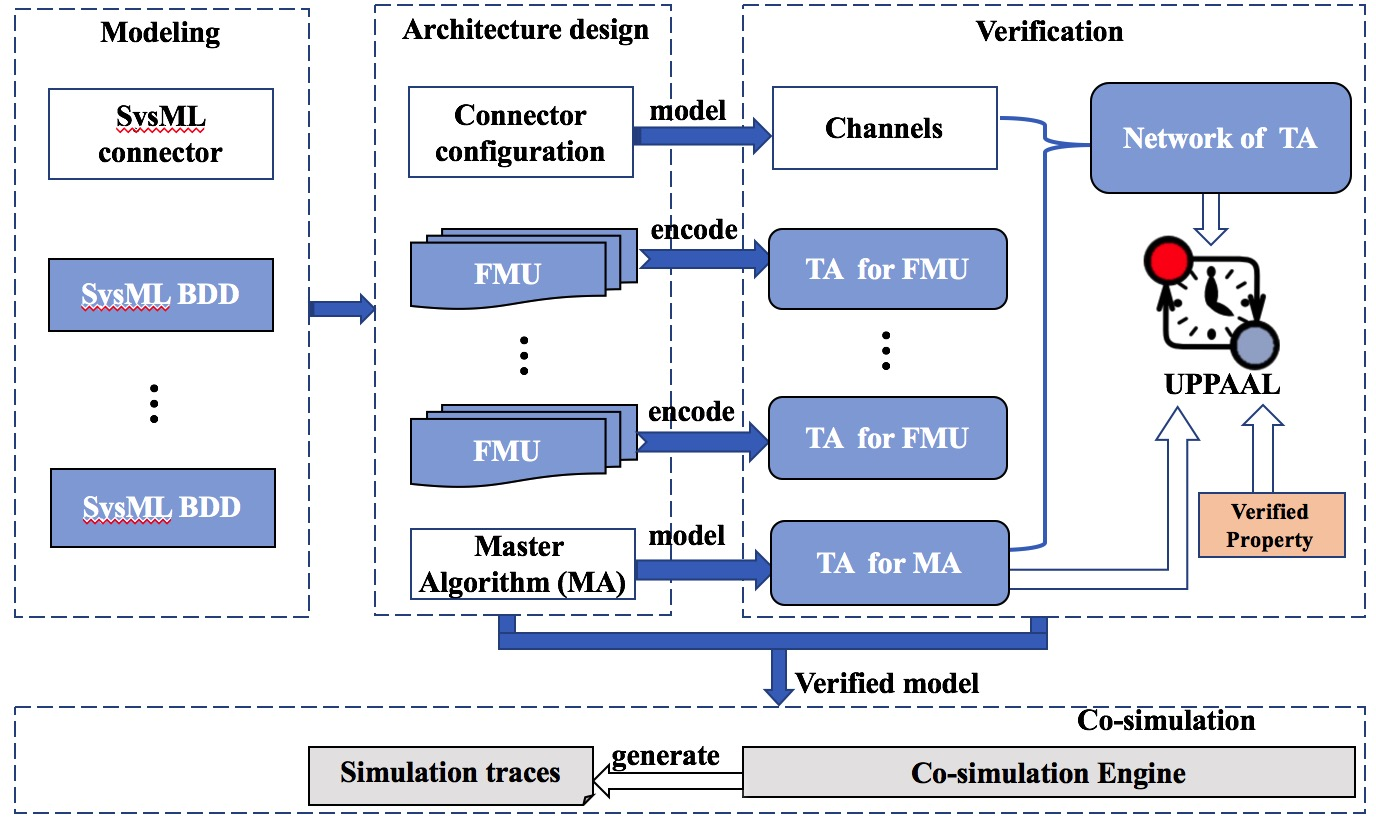
\includegraphics[width=6.0in]{fig/3/framework-3.jpg}}
	%\vspace{0.10in}
	\caption{协同行为正确性验证技术框架图}\label{fra-3}
\end{figure}
图\ref{fra-3}为异构系统协同行为正确性验证的技术框架图. 首先,我们在建模(Modeling)阶段使用SysML的BDD和IBD图来建模整个异构系统的架构。SysML的BDD中的块建模了异构系统的一个个组件;SysML的IBD图描述了各个块之间的连接关系。为了借助协同仿真技术对整个系统进行协同仿真,我们在架构设计(Architecture design)阶段将一个个块用FMU进行实现,同时将IBD图描述的关联关系转化为一个FMU之间的配置文件(Connector configuration)。接下来,我们自己设计了协同仿真的主算法(Master Algorithm,MA)来实现各个FMU之间的交互,同时来驱动协同仿真过程的执行。接下来是协同行为的验证(verification)阶段,也是我们本文的主要贡献点之一。为了验证协同行为的正确性,(1)我们先验证了协同仿真主算法的正确性:首先,我们用时间自动机对协同仿真的主算法进行形式化建模,然后将该时间自动机模型输入到UPPAAL模型检测工具中进行验证 (2)我们验证了整个系统协同行为的正确性:我们提出了一种从FMU到时间自动机的映射规则,我们根据此规则将FMU映射为时间自动机,接下来将FMU之间的配置文件转化为时间自动机的通道(Channels)。这样,我们就得到了一个时间自动机网络(Network of
TA):包括FMU映射成的时间自动机、主算法的时间自动机及各个时间自动机之间的通道)。最后我们将该时间自动机网络和要验证的属性(死锁、可达性、活性等)输入到UPPAAL中来验证该模型是否满足某些属性。一旦验证了协同行为的正确性,我们就可以将通过验证的模型输入到协同仿真的引擎之中进行协同仿真并得到协同仿真的迹。接下来,我们将详细介绍整个协同行为的验证过程。
\section{协同仿真主算法的验证}
在本小节我们首先介绍了三种协同仿真的主算法:固定步长算法、可回滚算法及可预测步长算法,之后我们用时间自动机形式化建模了这几种算法,最后将这几种算法的形式化模型输入到UPPAAL工具中,分别验证了这几种算法的有无死锁、可达性和活性的属性。
\subsection{协同仿真主算法介绍}
协同仿真的主算法用了调度和协同异构系统的多个	FMU组件的执行。每一个FMU都可以被看做一个可独自仿真的黑盒,但是多个FMU之间在某些特定的时刻需要进行数据交互和同步。图\ref{ad-fixedstep}描述了当前三种主要的协同仿真主算法的活动图。在接下来的内容中,我们对这三种算法进行简单的介绍。
\begin{figure}[htbp]
\centering{
		\subfigure[固定步长算法]{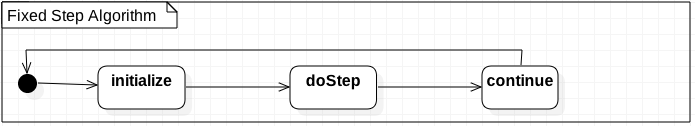
\includegraphics[width=4.5in,height=0.8in]{fig/3/MA1.png}
			\label{sd_fixedstep}}
		\hfil
		\subfigure[可回滚算法]{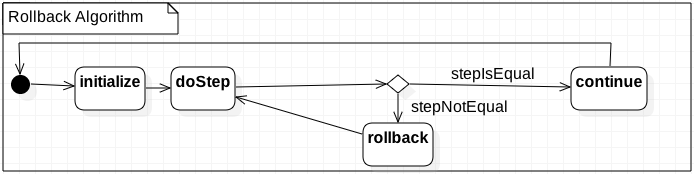
\includegraphics[width=4.5in,height=0.9in]{fig/3/MA2.png}
			\label{sd-rollback}}	
		\subfigure[可预测步长算法]{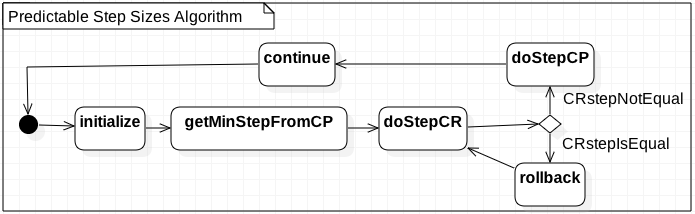
\includegraphics[width=4.5in,height=1.1in]{fig/3/MA3.png}
			\label{sd-pre}}		
	\caption{三种协同仿真主算法的活动图}
	\label{ad-fixedstep}
	}
\end{figure}
\subsubsection{固定步长算法}
对于固定步长算法\cite{BromanBGLMTW13},所有的FMU都有一个相同的步长。当协同仿真主算法在$t$时刻调用$doStep$函数执行步长$h$时,所有的FMU将从$t$时刻执行$h$步长并到达$t+h$时刻。在执行下一个$doStep$函数之前,要确保所有的FMU都执行完了上一个步长并且完成了数据交换。固定步长算法的活动图如图\ref{sd_fixedstep}所示,该活动图主要包含三个活动: $initialize$, $doStep$ 和 $continue$,首先对所有的FMU进行初始化,之后调用$deStep$函数进行仿真,最后在$continue$活动中完成FMU的数据交换。 在固定步长算法中,只要保证每个FMU的仿真是可靠的,则可以保证整个仿真过程的可靠性。但是,如果在某个FMU的仿真过程中出现错误,则会导致整个协同仿真过程出错。为了克服固定步长算法的缺陷,出现了可回滚的算法。
\subsubsection{可回滚算法}
FMI2.0相对于FMI1.0添加了几个重要的特性,它支持了对于FMU状态的保存和回滚。例如,主算法调用$FMU_{1}$和$FMU_{2}$的$doStep$函数执行$h$步长,但是$FMU_{1}$接受了该步长且$FMU_{2}$拒绝了该步长,则$FMU_{1}$和$FMU_{2}$都会执行$h$步长然后回滚到上一个时间点。可回滚算法的活动图如图\ref{sd-rollback}所示,相比固定步长算法,可回滚算法要求所有的FMU支持$rollback$方法, 且当某个FMU拒绝该步长时,所有的FMU将会回滚到上一个步长执行完之后的时间点。
\subsubsection{可预测步长算法}
如果可以预测FMU下一步能执行的最大步长(FMU在不错过事件时,能执行的仿真的最长时间),则可以大大提高协同仿真的效率。因此,论文\cite{BromanBGLMTW13}提出了$GetMaxStepSize$函数来预测FMU下一步能执行的最大步长,有了该函数的支持,就出现了可预测步长算法。图\ref{sd-pre}为可预测步长算法的活动图,首先,所有的FMU进行初始化,然后支持$GetMaxStepSize$函数的FMU在$getMinStepFromCP$活动中预测他们下一步能执行的最大步长,并且在所有的最大步长中选择最小的一个$h$作为所有FMU下一步执行的步长,之后所有的FMU执行$h$步长,如果所有的FMU都接受了该步长,则所有的FMU仿真该步长然后进行下一步。如果有FMU拒绝了该步长,则将所有的FMU回滚到上一个时间点,然后选择一个更小的步长进行仿真。
\subsection{协同仿真主算法的建模和验证} 
\label{sec:ma}
我们用时间自动机将三种不同类型的主算法进行形式化建模,图\ref{ta-master}是三种主算法的时间自动机模型。固定步长算法的时间自动机模型包含$Init$和$doStep$两个状态,且与$FMU$通过$continue$信道进行通信。 可回滚算法包括$Init$、$DoStep$和$Continue$三个状态。如果所有的FMU都接受了下一步要进行仿真的步长,则可回滚算法对应的时间自动机将发送$continue$信号,且迁移到$Continue$状态;否则,将发送$rollback$信号,且返回到上一个状态。可预测步长算法包括$Init$, $find \_ CP \_ MIN$, $DoStep$, $writeCP$四个状态。首先他们获得支持预测步长算法的多个FMU的最大步长,然后取所有最大步长的最小值$step1$ 。然后执行该步长,如果所有的FMU都接受则发送$continue$信号并迁移到下一个状态,否则发送$rollback$信号并回滚到$DoStep$ 状态。
\begin{figure}[htbp]
\centering{
		\subfigure[固定步长算法的时间自动机模型]{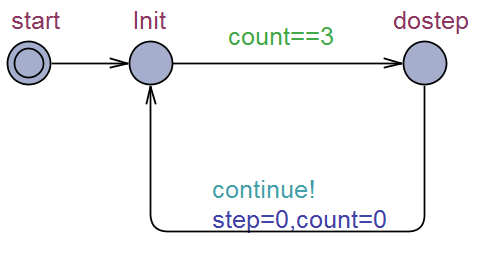
\includegraphics[width=1.5in,height=1.0in]{fig/3/fixedstep_master.png}
			\label{ta_fixedstep}}
		\hfil
		\subfigure[可回滚算法的时间自动机模型]{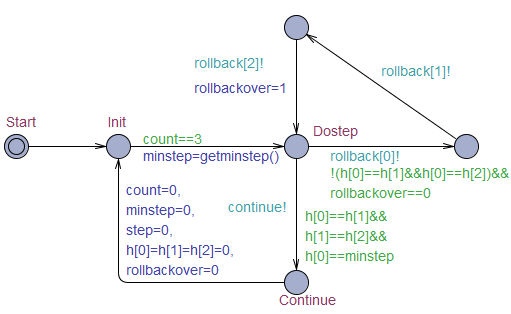
\includegraphics[width=2.5in,height=1.3in]{fig/3/rollback_master.png}
			\label{ta-rollback}}	
		\subfigure[可预测步长算法的时间自动机模型]{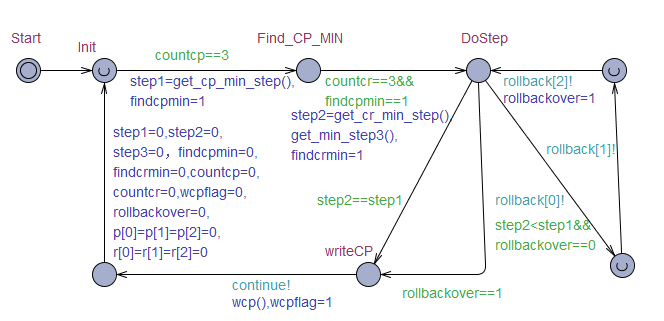
\includegraphics[width=4.5in,height=1.5in]{fig/3/pma_master.png}
			\label{ta-pre}}		
	\caption{三种不同主算法的时间自动机模型。}
	\label{ta-master}
	}
\end{figure}

UPPAAL是基于时间自动机理论对实时系统进行验证的工具,其中使用到的时间自动机模型增加了整型变量、多种数据类型及同步信号等扩展。我们使用UPPAAL工具验证了这三个模型的可达性、活性及死锁。具体的验证属性如下所示:
\begin{itemize}
\item
$E \langle\rangle master.dostep$, $E\langle\rangle master.Continue$ and $E\langle\rangle master.writeCP$是可达性验证,用来验证这些系统状态是否可达;
\item
$master.Init -> master.dostep$, $master.Init -> master.Continue$ and $master.Init -> master.Continue$是活性验证。如果主算法可以到达前一个状态,那么它最终也会到达后一个状态。
\item
$A[] not deadlock$ 是死锁的验证, 用来验证主算法是否存在死锁。
\end{itemize}
实验的结果如表\ref{ta_r}所示,从表中我们可以看出不存在死锁,且可达性和活性都满足,说明我们的主算法是正确的。例如:属性$A[]~not~deadlock$满足,说明主算法不存在死锁; 属性$E\langle\rangle~master.doStep$ 满足,说明系统最终会到达$doStep$状态。 总结来说,我们在这一小节验证了我们所用到的协同仿真的主算法的正确性。
\begin{table}
\caption{主算法的验证实验结果}
\centering
\begin{tabular}{c c c}
          \hline
          主算法 & 验证属性 & 结果\\
       \hline
        \multirow{2}{2.0cm}{固定步长}
                & $A[]~not~deadlock$ & True\\
                & $master.Init -> master.dostep$ & True\\
                & $E\langle\rangle~master.dostep$ & True\\

        \hline
        \multirow{2}{2.0cm}{可回滚}
                & $A[]~not~deadlock$ & True\\
                & $master.Init -> master.Continue$ & True\\
                & $E\langle\rangle~master.Continue$ & True\\

        \hline
        \multirow{2}{2.0cm}{可预测}
                & $A[]~not~deadlock$ & True\\
                & $master.Init -> master.writeCP$ & True\\
                & $E\langle\rangle~master.writeCP$ & True\\
        \hline
\end{tabular}
\label{ta_r}
\end{table}

\section{异构系统协同行为的验证}
在本小节,我们使用一个水箱的案例对整个协同行为的验证过程进行详细的描述。由于,在验证过程中,需要用时间自动机对FMU进行形式化描述,我们首先给出了从FMU到时间自动机的映射规则,然后我们使用SysML对整个系统进行架构设计,之后基于FMI标准对系统的各个组件进行实现,并给出多个FMU之间的连接关系配置,最后我们用时间自动机建模了FMU的形式化模型,并输入到UPPAAL工具中针对验证属性进行验证分析。
\subsection{FMU到时间自动机的映射} 
\label{sec:encode}
在本文的第二章的预备知识中,我们给出了FMU和时间自动机的语法及语义,下面我们根据第二章的语法语义给出FMU和时间自动机的映射关系。我们发现FMU和时间自动机的语义之间存在一定的关联。FMU的语义关注于FMU的执行序列,也就是状态随着时间的不断迁移;因此,时间自动机的执行迹跟FMU的执行序列十分相似,也是状态随着时间的迁移序列。因此,我们使用时间自动机来对FMU进行形式化描述,从而来分析多个FMU之间的协同行为。
给定一个FMU$F=(S,U,Y,D,s_{0},set,get,doStep)$, 我们可以根据他们执行语义之间的关联,将FMU用时间自动机$\textit{A}=(L,l_{0},E,I)$进行形式化描述:
\begin{itemize}
\item
$L$是时间自动机的有限位置集合。因此,时间自动机语义模型$L_{\textit{A}}$中的状态可以看做为FMU中的状态,即$(l,v) \Rightarrow s$。
\item
时间自动机语义模型$L_{\textit{A}}$中的初始状态可以看做为FMU中的初始状态, 即$(l_{0},v_{0}) \Rightarrow s_{0}$。
\item
FMU中的输入变量$u \in U$可以看做为时间自动机的$Act_{i} \cup \{absent\}$。
\item
FMU的输出变量$y \in Y$可以看做为时间自动机的$Act_{o} \cup \{absent\}$。
\item
时间自动机的输入动作$e \in Act_{i}$可以看做FMU中的$set$函数。
\item
时间自动机的输出动作$e \in Act_{o}$可以看做为FMU中的$get$函数。  
\item
时间自动机之间依靠channel的同步可以看做为FMU之间的依赖关系。 $(u,y) \in D$表示输出变量$y$依赖于输入变量$u$,在时间自动机中输出动作同样依赖于输入动作。
\item
对于时间自动机,一个动作$e \in Act$会触发一个迁移$s \xrightarrow{e} s^{\prime}$, 这个过程就相当于FMU里面的$doStep$执行,会使其到达下一个状态。 例如:时间自动机的迁移$l \xrightarrow{e} l^{\prime}$可以描述FMU的$doStep(s,h)$被调用,并且此FMU接受了步长$h$并到达了下一个状态 $s^{\prime}$;然而,此FMU也可能会拒绝步长$h$, 并且发生了回滚,这个过程在时间自动机里面可以用一条边$l^{\prime} \xrightarrow{e} l$来进行描述,来表示回滚到了上一个状态。

\end{itemize}
\begin{figure}[htbp]
	\centering	{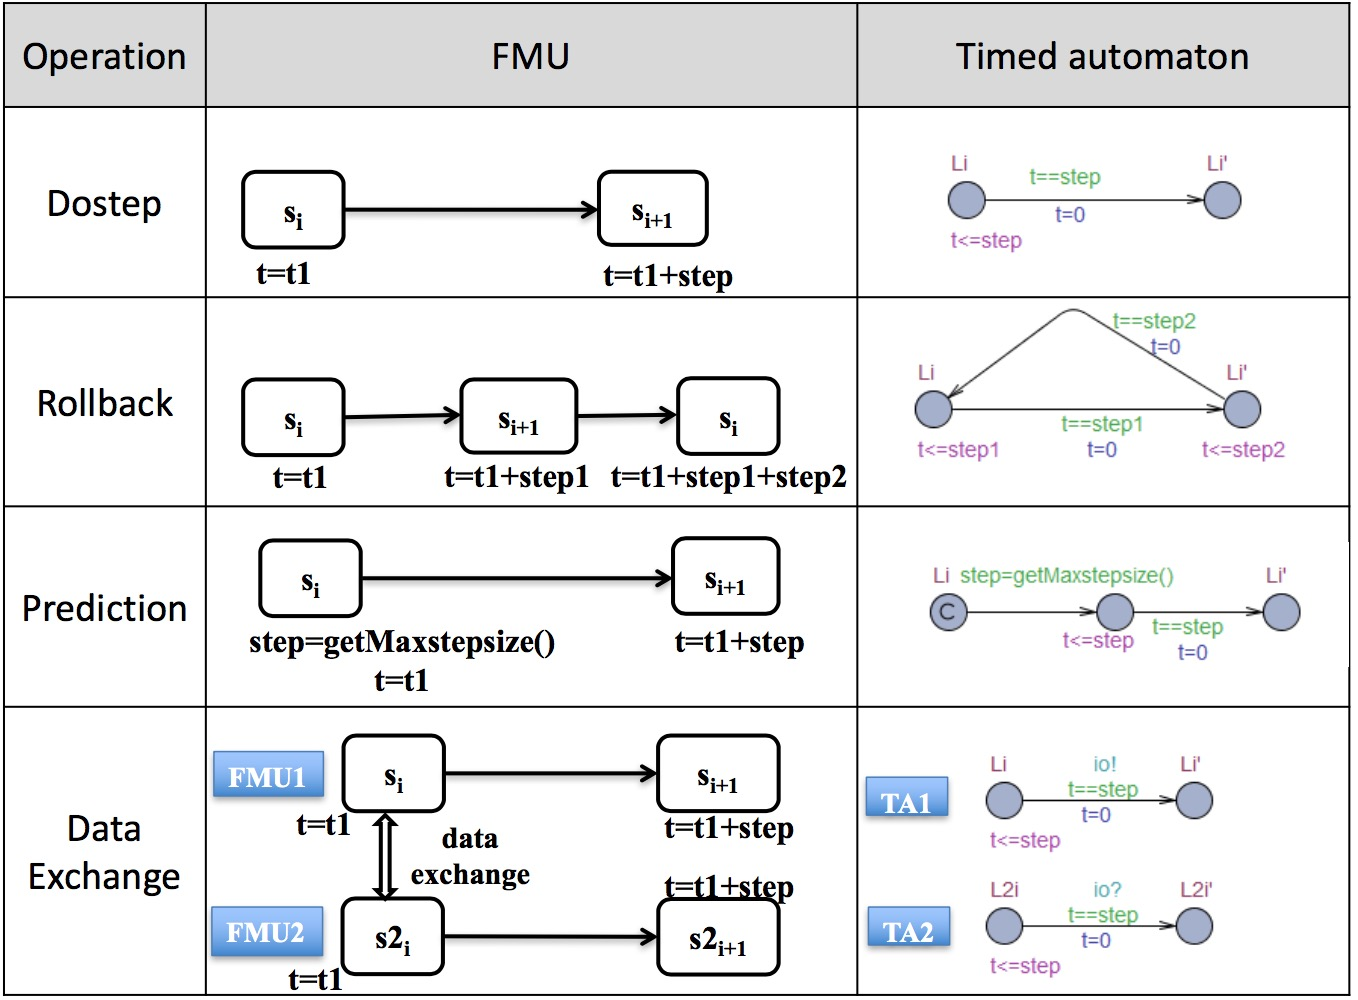
\includegraphics[width=5.0in,height=3.5in]{fig/3/abstractRole.png}}
	\caption{Encoding rules from FMU to TA.}
	\label{fmutota}
\end{figure}

将FMU直接转化为时间自动机是比较难得,S. Tripakis层在论文 \cite{Tripakis15}中将时间自动机编码为FMU。我们受到此论文的启发,根据时间自动机和FMU之间语义的关联,提出了几条从FMU到时间自动机在操作语义上的映射规则如图\ref{fmutota}所示。

给定FMU$t_{1}$时刻的当前状态$s_{i}$,操作函数$Dostep$可以使得FMU在$t_{1}+step$时刻到达$s_{i+1}$状态。这个操作可以用时间自动机的迁移来进行表示:在位置$L_{i}$延迟$step$的时间并迁移到一个新的位置$L_{i}^{\prime}$。

对于操作函数$Rollback$,给定FMU$t_{1}$时刻的当前状态$s_{i}$,FMU首先执行步长$step1$并在 $t_{1}+step1$时刻到达$s_{i+1}$状态,然后操作函数$rollback$又使得FMU回滚到上一个状态$s_{i}$。对于时间自动机来说,这个可以表示为在$L_{i}$位置延迟了$step1$时间单位并迁移到新的位置 a$L_{i}^{\prime}$,之后又迁移到了上一个位置$L_{i}$。 

对于操作函数$Prediction$,给定一个状态$s_{i}$, FMU可以由一个函数$getMaxstepsieze$得到下一步能执行的最大步长,然后执行此步长并在$t_{1}+step$时刻到达 $s_{i+1}$状态。 对于时间自动机,可以表示为在$L_{i}$位置执行了一个函数并得到要延迟的时间 $step$, 然后延迟该时间单位并迁移到一个新的位置 $L_{i}^{\prime}$ .

对于操作函数$Data Exchange$,两个FMU在$t_{1}$时刻的$s_{i}$状态执行$Data Exchange$进行了数据交换, 然后他们执行相同的步长并迁移到下一个位置$s_{i+1}$和$s2_{i+1}$。对于时间自动机,可以表示为两个时间自动机在$t_{1}$时刻通过信道$io$进行了同步,然后延迟了相同的时间并$L_{i}$位置迁移到$L_{i+1}$位置。

为了将FMU用时间自动机进行形式化描述,我们提出了以上操作语义的映射规则。为了证明我们以上规则的正确性,我们分析了FMU和时间自动机的执行片段如下所示:
\begin{itemize}
\item
对于操作函数$Dostep$的映射,在FMU和时间自动机中的执行片段为 ($s_{i}$, $t_{1}$), ($s_{i+1}$, $t_{1}+step$)和($l_{i}$, $t$), ($l_{i}^{\prime}$, $t+step$). 这说明时间自动机和FMU都执行 $step$的时间单位并到达了一个新的状态或是位置。
\item 
对于操作函数$Rollback$的映射, 在FMU和时间自动机的执行片段为($s_{i}$, $t_{1}$), ($s_{i+1}$, $t_{1}+step1$), ($s_{i}$, $t_{1}+step1+step2$) 和 ($l_{i}$, $t$), ($l_{i}^{\prime}$, $t+step1$), ($l_{i}$, $t+step1+step2$)。这说明时间自动机和FMU都首先执行了$step1$时间单位,并且到达了一个新的状态或位置,然后执行了$step2$时间单位, 又返回到了之前的状态或位置。
\item
对于操作函数$Prediction$的映射,FMU和时间自动机的执行片段为($s_{i}$, $t_{1}$), ($s_{i+1}$, $t_{1}+step$)和($l_{i}$, $t$), ($l_{i}^{\prime}$, $t+step$). 这说明时间自动机和FMU都成功预测到了步长$step$并执行了此步长。
\item
对于操作函数$Data Exchange$的映射,FMU1和时间自动机TA1的执行片段为 ($s_{i}$, $t_{1}$), ($s_{i+1}$, $t_{1}+step$)和($l_{i}$, $t$), ($l_{i}^{\prime}$, $t+step$)。FMU2和时间自动机TA2的执行片段为 ($s2_{i}$, $t_{1}$), ($s2_{i+1}$, $t_{1}+step$) 和 ($l2_{i}$, $t$), ($l2_{i}^{\prime}$, $t+step$)。这说明时间自动机和FMU在经过了数据交换后又执行了$step$时间单位。
\end{itemize}
为了更加准确的验证映射规则的正确性,我们分析了时间自动机和FMU的整个执行序列。我们通过分析得到FMU和时间自动机的执行序列是等价的,验证了映射规则的正确性。在之后几个小节的内容中,我们将此映射规则应用到了水箱的案例中,根据我们之后对案例仿真片段的分析,我们也发现映射规则是正确的。 
\subsection{基于SysML的架构建模} 
为了更好的阐述我们的方法,我们采用了水箱的案例 \cite{•} 作为驱动以更加形象的展示我们的方法。下面我们先简单的介绍一下水箱案例,然后用SysML建模语言对整个案例的架构建模。水箱案例:有一个水源可以向水箱里面注水,且水箱里面的水通过一个管道流入到一个水池当中,这个水源的流出由一个阀门控制,而阀门的开关由一个控制器进行控制。在本小节,由于水箱、阀门、控制器连接方式的不同,我们在此描述了三种不同类型的水箱系统。

SysML是为模型驱动式软件开发(Model-Based Systems Engineering,MBSE)\cite{Dori16}而提出的一种通用的领域建模语言( Domain-Specific Language,DSL)\cite{SemerathBHSV17} ,它起源于国际系统工程委员会(INCOSE)的倡议\ cite {Pepper2015International}并于2001年1月发布 。SysML的BDD图用块来描述系统中组件的结构;IBD图用来描述各个块之间的关联关系。各个块的接口由连接器进行关联,因此,系统各个组件的依赖关系可以用各个块的接口之间的连接进行表示。

图\ref{myad}是水箱案例的SysML BDD图,其中包含三个块: $Valve$, $Tank$ 和 $Controller$。 $Valve$和$Tank$是物理组件;$Controller$是信息组件。每一个组件都有自己的输入和输出接口,例如:$Valve$的输入接口是$vin$,它用来输入阀门的开关$OpenClosed$信号。
\begin{figure}[htbp]
	\centering	{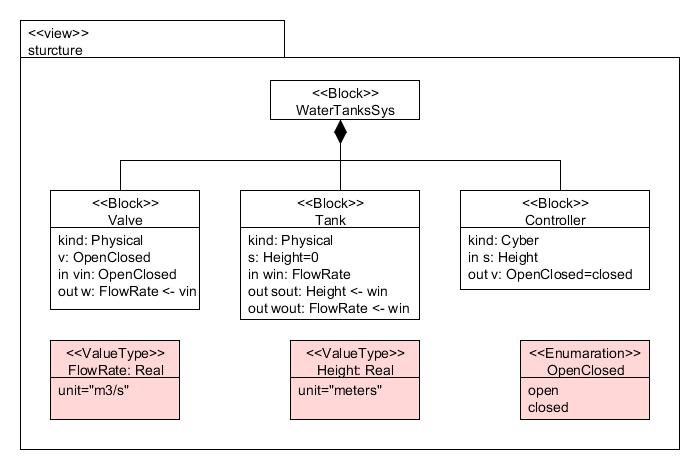
\includegraphics[width=4.5in,height=3.0in]{fig/3/AD.jpg}}
	\caption{水箱系统的SysML BDD}
	\label{myad}
\end{figure}

图\ref{cd} 是SysML的IBD图,在这里我们给出了三种连接情形。在第一种情形中,系统包含一个阀门、一个控制器和一个水箱,控制器随机的给阀门发送开关信息,导致水箱中的水位不断的变化;在第二种情形中,控制器信号的发送受到水箱水位的影响,控制器根据水箱的水位发送开关信号;在第三种情形中,我们添加了一个水箱$waterTank2$,水箱$waterTank1$中的水通过管道先流入$waterTank2$中,最后流入水池。

\begin{figure}[htbp]
\centering{
		\subfigure[情形1]{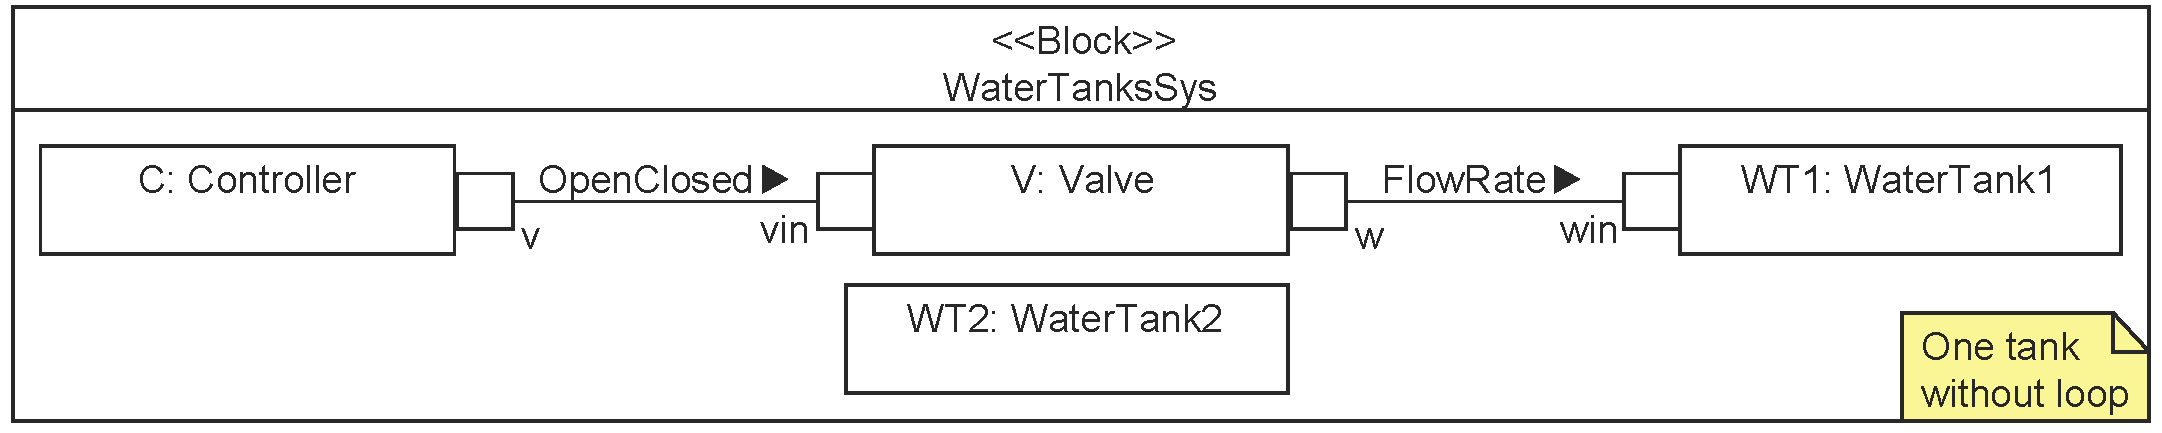
\includegraphics[width=4.5in,height=1.0in]{fig/3/CD1.png}
			\label{cd1}}
		\hfil
		\subfigure[情形2]{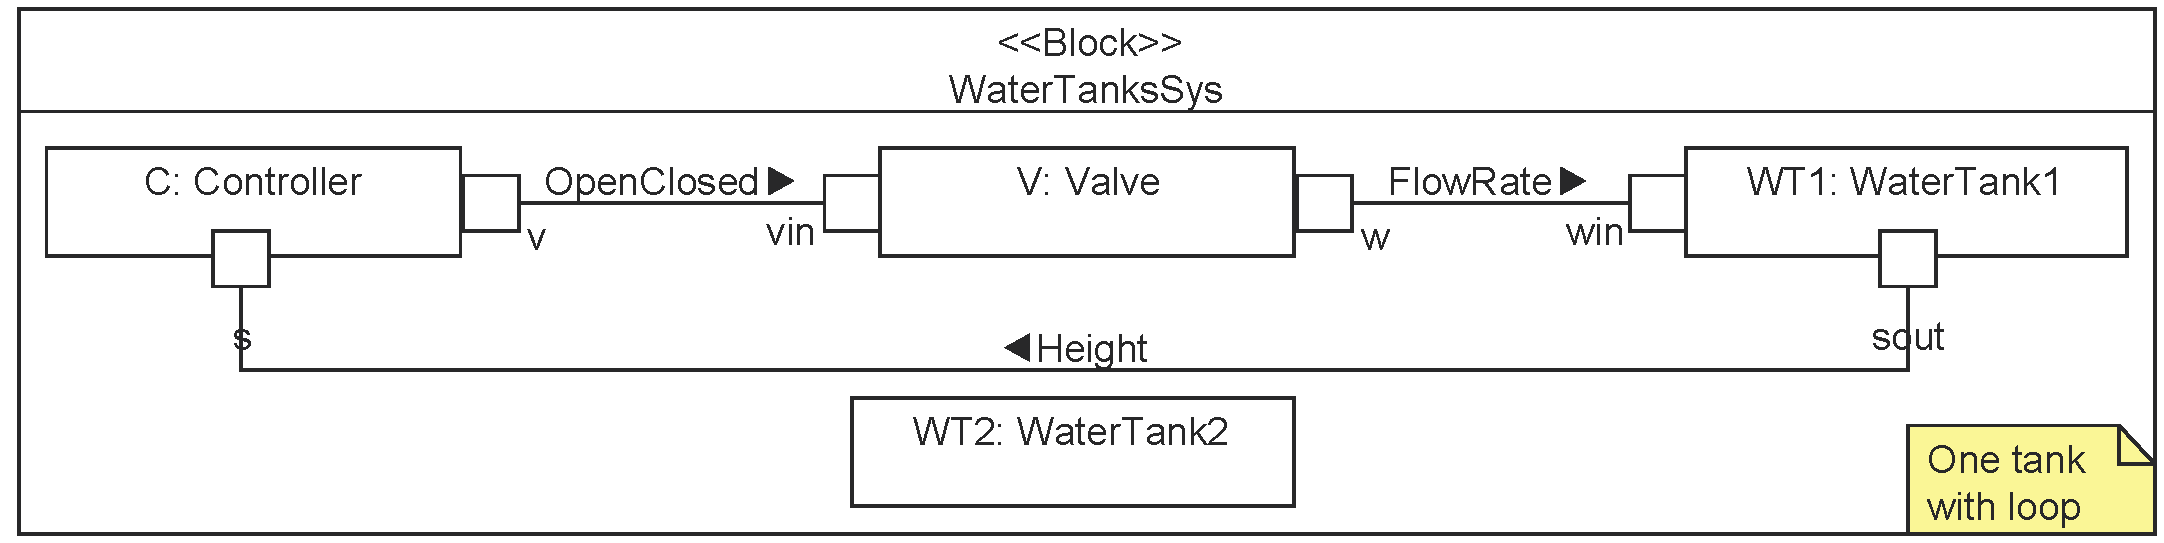
\includegraphics[width=4.5in,height=1.0in]{fig/3/CD2.png}
			\label{cd2}}
		\hfil
		\subfigure[情形3]{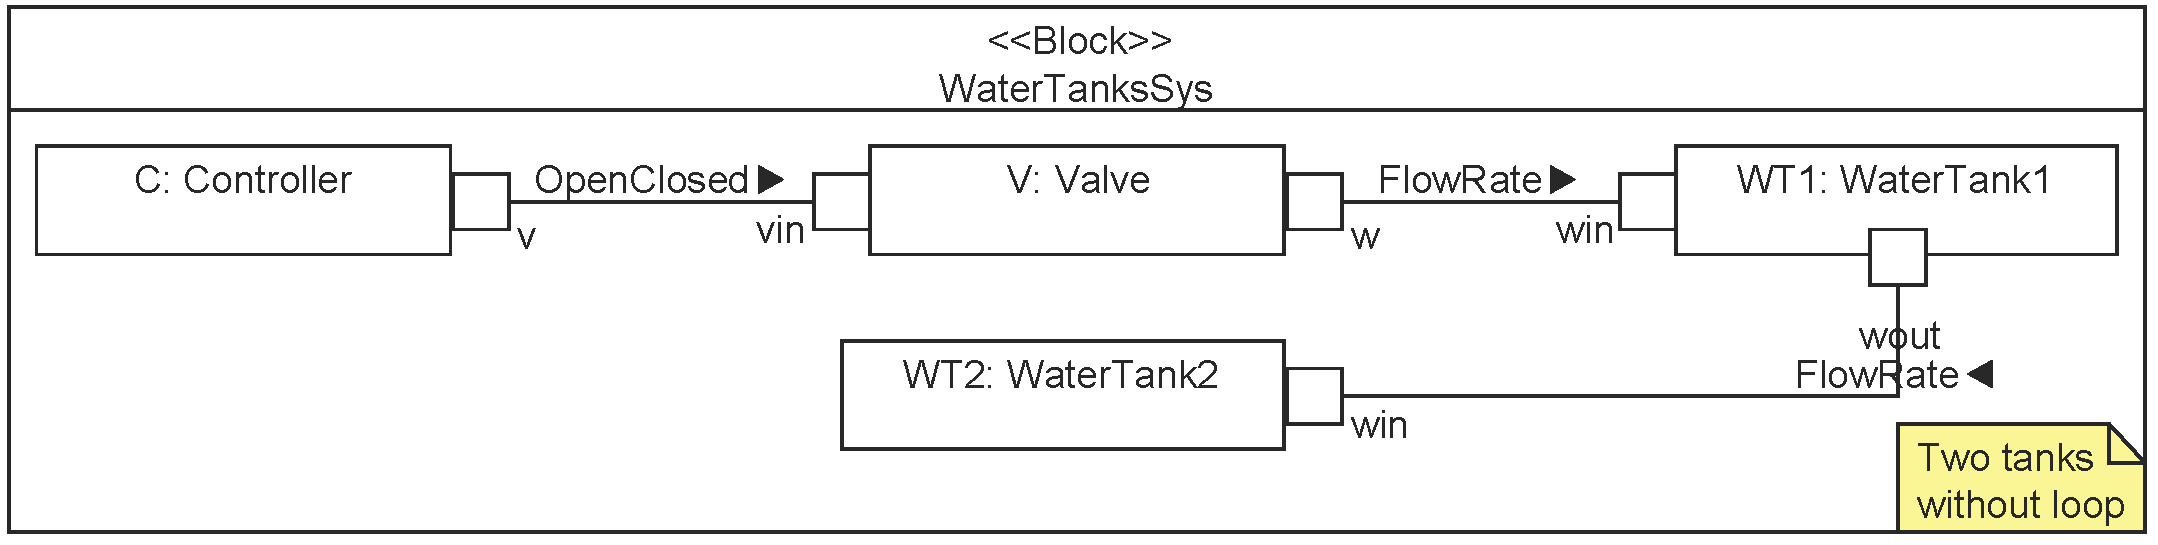
\includegraphics[width=4.5in,height=1.0in]{fig/3/CD3.png}
			\label{cd3}}
	\caption{水箱系统的SysML IBD}
	\label{cd}
	}
\end{figure}
在本小节我们用SysML BDD图描述了系统组件的结构,并用SysML的IBD图描述了各个组件之间的连接。在下一个小节,我们基于FMI标准用FMU来实现每一个系统组件,并将SysML IBD中描述的关联关系用一个FMU之间的接口配置文件进行表示。
\subsection{基于FMI的连接关系配置} 
\label{sec:case}
图\ref{fmu-con}描述的是水箱系统中的FMU组件及各个FMU之间的连接。根据图\ref{cd}给定的SysML IBD,我们也得到了三种FMU的情形。第一种情形如图\ref{fmu-con1}所示,系统中有三个FMU组件:$Controller$, $Valve$ 和$WaterTank1$和两个接口$v \_ vin$及$w \_ win$。 $Controller$ 和 $Valve$由$v \_ vin$接口连接; $Valve$ 和 $WaterTank1$ 由 $w \_ win$接口连接。第二种情形如图 \ref{fmu-con2}所示,其中在第一种情形上添加了$WaterTank1$ 和$Controller$的接口$sout \_ s$,表示控制器信号的发送受到水箱$WaterTank1$的水位影响。 图\ref{fmu-con3}是第三种情形,在第一种情形上添加了另一个水箱$WaterTank2$, 水箱$WaterTank1$ 和$WaterTank2$由接口$w \_ out$连接。 
\begin{figure}[htbp]
\centering{
		\subfigure[情形1]{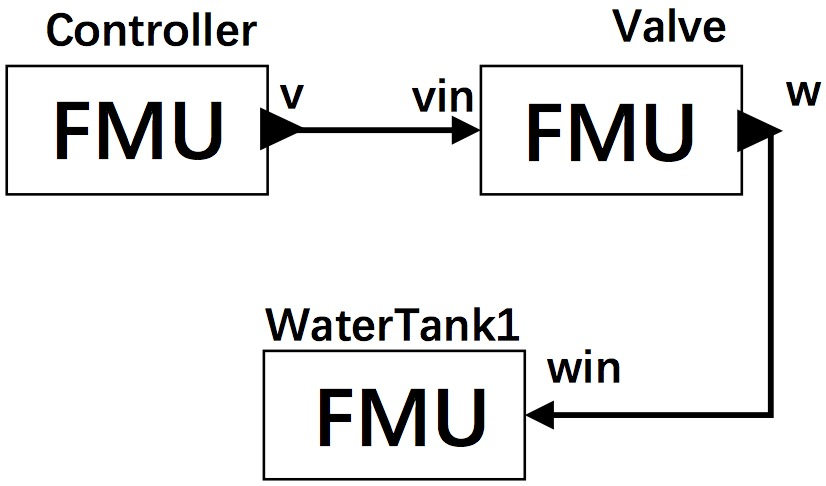
\includegraphics[width=1.5in,height=0.9in]{fig/3/fmuc1.png}
			\label{fmu-con1}}
		\hfil
		\subfigure[情形2]{\includegraphics[width=1.5in,height=0.9in]{fig/3/fmuc2.png}
			\label{fmu-con2}}
		\hfil
		\subfigure[情形3]{\includegraphics[width=1.5in,height=0.9in]{fig/3/fmuc3.png}
			\label{fmu-con3}}
	\caption{水箱系统中FMU的三种连接情形}
	\label{fmu-con}
	}
\end{figure}

在本小节我们设计了FMU及FMU之间的连接,我们只需要添加一个协同仿真的主算法就可以在协同仿真引擎当中对整个异构系统进行协同仿真并得到仿真迹。但是,在进行仿真之前,我们要保证各个FMU之间协同行为的正确性,因此,我们在下一个小节基于时间自动机理论对系统的协同行为进行验证,这也是我们本文的主要贡献点之一。
\subsection{协同行为的验证分析} 
\label{sec:mauppaal}
在本小节我们基于时间自动机理论对水箱系统中组件之间的协同行为的正确性进行验证。首先我们根据小节\ref{sec:encode}中提出的映射规则,将水箱系统中的FMU用时间自动机进行形式化描述,并取小节\ref{sec:ma}中建模的一个主算法(在此,采用可回滚算法作为主算法,其他算法的验证分析与该算法类似,在此不做描述),FMU之间的接口配置文件我们用时间自动机之间的信道进行描述。由此,我们得到了一个由主算法、FMU的时间自动机模型及由配置文件转化得到的信道组成的时间自动机网络。图\ref{tk-arch1}为上述小节中情形1的时间自动机网络模型。

\begin{figure}[htbp]
\centering{
		\subfigure[FMU\_controller 的时间自动机模型]{\includegraphics[width=1.6in,height=1.0in]{fig/3/2signal_controller.png}
			\label{tk_controller}}
		\hfil
		\subfigure[FMU\_valve 的时间自动机模型]{\includegraphics[width=1.6in,height=1.0in]{fig/3/2signal_v.png}
			\label{tk_v}}
			
	    \subfigure[FMU\_WaterTank1 的时间自动机模型]{\includegraphics[width=1.5in,height=1.2in]{fig/3/2signal_wt1.png}
			\label{tk_wt1}}
		\hfil
		 \subfigure[可回滚主算法的时间自动机模型]{\includegraphics[width=1.7in,height=1.2in]{fig/3/2signal_master.png}
			\label{tk_ma}}		
	\caption{情形1的时间自动机网络: $controller$ $\vert\vert$ $valve$ $\vert\vert$ $WaterTank1$ $\vert\vert$ $MA$.}
	\label{tk-arch1}
	}
\end{figure}

\begin{figure}[htbp]
\centering{
		\subfigure[部分迹]{\includegraphics[width=1.6in,height=2.0in]{fig/3/trs.png}
			\label{trs}}
		\hfil
		\subfigure[执行序列图]{\includegraphics[width=1.6in,height=2.0in]{fig/3/seq.png}
			\label{seq}}
	\caption{协同过程在UPPAAL中的执行序列。}
	\label{trs-seq}
	}
\end{figure}

图\ref{tk_controller}, \ref{tk_v}, \ref{tk_wt1}分别是$controller$, $valve$ 和 $WaterTank1$的时间自动机模型。这些自动机都有四个主要的位置:$start$, $dostep$, $Rollback$和$reset$。图\ref{tk_controller}是 $controller$的时间自动机模型,它首先通过信道 $v$与$valve$的时间自动机模型进行交互并到达$Rollback$状态,然后等待主算法的信号,直到它收到了来自主算法的$continue$信号再与其他的FMU进行数据交互并到达$start$状态;否则,它收到$rollback$信号,并回到$Rollback$状态。$valve$和$WaterTank1$的时间自动机中位置和迁移与 $controller$类似。图\ref{tk_ma} 是主算法的时间自动机模型,首先主算法先进性参数初始化,然后根据条件来判断发出  $continue$信号或是$rollback$信号。

图\ref{trs-seq}是协同过程在UPPAAL中的执行片段,我们可以看到 $valve$ 首先发送了信号$w$ 来与 $WaterTank1$进行数据交换,然后,$WaterTank1$ 到达了 $dostep$ 状态,之后主算法广播  $rollback$信号导致FMU到达$reset$状态,最后主算法发送$continue$ 信号使得所有的FMU到达 $start$状态并开始下一步仿真。通过对执行序列的分析,我们发现模型可以正确仿真。

为了比较小节\ref{sec:case}中描述的三种情形的协同行为,我们同时用时间自动机形式化描述了其他两种情形。对于第二种情形,我们在第一种情形基础上添加了$controller$ 和 $WaterTank1$之间的信道$s$如图\ref{tk-arch2}所示;对于第三种情形我们建模了$WaterTank2$的模型并添加了信道$w2$ 如图Fig.\ref{arc3}所示。其他的模型与第一种情形中的模型类似,我们在此只给出了新增加的或有改动的模型。接下来我们将对这三种情形进行验证。
\begin{figure}[htbp]
\centering{
		\subfigure[TA for FMU\_controller]{\includegraphics[width=1.8in,height=1.2in]{fig/3/2signal_cycle_controller.png}
			\label{tk2_controller}}
		\hfil
		\subfigure[TA for FMU\_WaterTank1]{\includegraphics[width=1.5in,height=1.2in]{fig/3/2signal_cycle_wt1.png}
			\label{tk2_v}}		
	\caption{TA for connection case 2.}
	\label{tk-arch2}
	}
\end{figure}
\begin{figure}[htbp]
	\centering	{\includegraphics[width=3.5in,height=1.2in]{fig/3/4signal_wt2.png}}
	\caption{TA for FMU\_WaterTank2 of connection case 3.}\label{arc3}
\end{figure}

我们对每一种情形都验证了以下属性:
\begin{itemize}
\item
$E\langle\rangle~WT1.Rollback$和 $E\langle\rangle~master.Continue$ 为可达性验证,它表示$WaterTank1$将到达$Rollback$状态 且主算法会到达 $Continue$状态。
\item
$master.start -> master.Continue$为活性验证,它表示一旦主算法开始,它最早会到达 $Continue$状态.
\item 
$A[]~not~deadlock$为死锁的验证,它用来验证系统有无死锁。
\end{itemize}

验证结果如表\ref{rs}所示,我们发现情形1和情形3的验证属性都满足,它表示该情形的协同是正确的。然而情形2的可达性和活性不满足,是由于在该模型中出现了环路依赖,我们需要消除该环路依赖再进行下一步的仿真,在本文中我们只关注协同行为的验证,对于如何消除环路依赖在接下来的工作中我们会做进一步研究。 
\begin{table}
\caption{三种情形的验证结果}
\centering
\begin{tabular}{c c c} 
        \hline  
        情形 & 验证属性 & 结果\\
        \hline
        \multirow{2}{2.0cm}{情形1}  
                & $E\langle\rangle~WT1.Rollback$ & True\\ 
                & $E\langle\rangle~master.Continue$ & True\\ 
                & $master.start -> master.Continue$ & True\\ 
                & $A[]~not~deadlock$ & True\\   
        \hline 
        \multirow{2}{2.0cm}{情形2}  
                & $E\langle\rangle~WT1.Rollback$ & True\\ 
                & $E\langle\rangle~master.Continue$ & False\\ 
                & $master.start -> master.Continue$ & False\\ 
                & $A[]~not~deadlock$ & True\\   
        \hline 
        \multirow{2}{2.0cm}{情形3}  
                & $E\langle\rangle~WT1.Rollback$ & True\\ 
                & $E\langle\rangle~master.Continue$ & True\\ 
                & $master.start -> master.Continue$ & True\\ 
                & $A[]~not~deadlock$ & True\\   
        \hline 
\end{tabular} 
\label{rs}
\end{table}

\section{本章小结}
在本小节我们提出了一种新的方法来验证异构系统协同行为的正确性,我们首先用SysML建模语言建模了整个系统的架构,然后基于FMI标准对整个架构进行实现。之后提出了一种映射规则将FMU用时间自动机进行了形式化描述,最后基于时间自动机理论对整个系统的协同行为的正确性进行了验证。经过本小节的验证,我们可以得到通过验证的基于FMI标准的模型,该模型可以在协同仿真引擎中直接仿真并得到仿真迹,在下一个小节,我们将提出一种高效的统计模型检测方法,针对某些验证属性对协同仿真的迹进行定量的评估。
\chapter{基于分布式统计模型检测的异构系统验证分析}
\label{ch4}

%\section{基于FMI的协同仿真}
%\section{验证属性设计}
\section{基于抽象和学习的分布式统计模型检测}
\section{异构系统验证分析}

\section{本章小结}

\chapter{工具实现}
\label{ch5}

\section{异构系统验证分析工具(Co-SMC)介绍}
在本文我们提出了一种面向异构系统的验证分析方法,该方法基于协同仿真和统计模型检测,实现对异构系统行为的验证、分析。为了对该方法提供支持,我们设计、开发了异构系统验证分析工具,该工具主要由协同仿真、统计模型检测器及统计分析器三部分组成。在协同仿真器模块中,用户可以输入要进行协同仿真的多个FMU模型,然后设置仿真步长和多个FMU模型之间的参数对应关系,最后,可以从4种协同仿真算法中选择适当的协同仿真算法,对系统模型进行协同仿真并产生协同仿真的迹。统计模型检测器模块以协同仿真器产生的迹为输入,然后设置需要验证的属性,最后选择适合的统计模型检测算法进行定量的验证分析。用户可以在统计分析器模块对协同仿真器产生的迹或是统计模型检测器产生的验证结果进行统计分析,并绘制出饼状图、折线图等可视化的图形,有利于对模型的各种行为进行更加直观的分析。接下来我们对Co-SMC工具的各个部分进行详细的描述。
\begin{figure}[htbp]
	\centering
	{\includegraphics[width=4.0in]{fig/5/tool1.png}}
	%\vspace{0.10in}
	\caption{Co-SMC协同仿真器}\label{tool-1}
\end{figure}
\begin{figure}[htbp]
	\centering
	{\includegraphics[width=4.0in]{fig/5/tool2.png}}
	%\vspace{0.10in}
	\caption{Co-SMC统计模型检测器}\label{tool-2}
\end{figure}
\begin{figure}[htbp]
	\centering
	{\includegraphics[width=4.0in]{fig/5/tool3.png}}
	%\vspace{0.10in}
	\caption{Co-SMC协同仿真器}\label{tool-3}
\end{figure}
图\ref{tool-1}是Co-SMC工具的协同仿真器,该工具主要包括
\section{Co-SMC程序实现}


\section{本章小结}

\chapter{案例分析与实验评估}
\label{ch6}
在本小节,我们使用两个案例(智能温控系统和机器人路径规划系统)来展示本文提出的方法的有效性。首先,我们使用SysML建模语言对这案例进行建模并根据基于FMI标准进行实现以得到基于FMI标准的仿真模型,然后我们使用章节3提出的方法对系统行为的正确性进行验证,之后将验证通过的模型进行协同仿真并将得到仿真迹用章节4提出的方法进行评估分析得到最终的评估结果。由于在章节3中我们已经使用了水箱的对整个方法进行了详细的描述,因此在本章节的案例中我们不对章节3涉及的过程做过多的描述,而是重点关注模型通过统计模型检测算法验证之后得到的评估结果及章节4提出的经过改进的算法的准确度及效率问题。
\section{案例一:智能温控系统}
智能温控系统\cite{•}在当今社会能源节约问题上起到十分重要的作用。该系统主要包含五个部分:\emph{房间温度,控制器,室外温度,加热器及用户}。控制器根据用户的行为及室内温度来控制加热器的开关,室内温度又受到室外温度、加热器及用户行为的影响。该系统的主要目的是评估某种控制策略下房间温度的舒适度及整个系统的能耗。
\subsection{系统建模与设计}

\subsection{系统验证分析}
本实验的分布式环境为五台处理器为英特尔(TM) i7-4790 (八核,主频3.6G赫兹)组成的集群。为了评估系统的行为和算法的性能,我们验证了以下三个验证属性如表 \ref{tb:property}所示。
\begin{table}[t]
	\caption{智能温控系统的验证属性}
	\label{tb:property}
	\centering
	\begin{tabular}{c c c c}
		\hline
		序号 &  $(\delta,c)$ & 验证属性 & 验证结果 \\
		\hline
		$\phi_1$ & $(0.05,0.99)$  & $P_{=?}(F^{\leq48}~energy \geq 210)$ & 0.1778 \\ 
		$\phi_2$ & $(0.01,0.99)$  & $P_{=?}(F^{\leq48}~discomfort \geq 15)$ & 0.4861\\
		$\phi_3$ & $(0.02,0.9)$ & 
		\tabincell{c}{$P_{=?}(F^{\leq48}~ discomfort \leq 15$ \\ $\wedge~energy \geq 170)$} & 0.4535 \\
		\hline
	\end{tabular}
\end{table}
我们采用贝叶斯区间估计算法对上属三条验证属性进行评估分析以得到的验证结果。下面我们对表\ref{tb:property}的验证属性及验证结果进行分析:(1)$\phi_1$用来评估在48小时内能耗超过210的概率大小,我们得到的验证结果为0.1778,表示在48小时内系统能耗超过210的可能性比较小;(2)$\phi_1$用来评估48小时内,系统的不舒适度大于15的概率,得到的验证结果为0.4861;(3)$\phi_3$用来评估在48小时内,系统的不舒适度小于15且能耗大于170的概率,得到的验证结果为0.4535。由此,可以发现本文提出的技术方法可以有效的评估异构系统的行为。

\subsection{算法评估分析}
为了评估章节4提出的算法效率,在本小节我们针对以上的三个验证属性,从产生的迹的数量,验证所需要的时间及验证误差三个方面对比了多种统计模型检测算法:贝叶斯区间估计算法(BIE)、分布式的贝叶斯区间估计算法(DBIE)、基于抽象和学习的分布式统计模型检测算法(DAL-SMC)、经过优化的基于抽象和学习的分布式统计模型检测算法(DAL-SMC opt)、分布式的APMC\cite{•}算法(DAPMC),算法对比结果如图\ref{rs_sb}所示。
\begin{figure*}[htbp]
\centering{
		\subfigure[产生的迹的数量]{\includegraphics[width=1.5in,height=1.3in]{fig/4/sb-trace.png}
			\label{trace_sb}}
		\hfil
		\subfigure[验证时间]{\includegraphics[width=1.5in,height=1.3in]{fig/4/sb-time.png}
			\label{time_sb}}
		\hfil
		\subfigure[验证误差]{\includegraphics[width=1.5in,height=1.3in]{fig/4/sb-error.png}
			\label{error_sb}}
	\caption{智能温控系统案例算法对比}
	\label{rs_sb}
	}
\end{figure*}

图\ref{trace_sb}是算法产生的迹的数量对比,我们可以发现对于验证属性$\phi_2$,DAPMC将消耗200000条迹,然而DBIE只需要20000条迹。 DAL-SMC和 DAL-SMC opt.需要更少量的迹(大约10000条)。 算法的验证时间的对比如图 \ref{time_sb}所示,对于验证属性$\phi_2$,BIE需要6000秒,但分布式的BIE只需要大约250秒,DAL-SMC和DAL-SMC opt.需要更少的时间。图\ref{error_sb} 是算法的验证误差分析,对于验证属性$\phi1$,分布式BIE和DAPMC的误差大约为 0.013,DAL-SMC和DAL-SMC的验证误差大约为0.045和0.032。更详细的实验数据如表\ref{ta-rs}所示。 

\section{案例二:机器人路径规划系统}
在近些年来,机器人路径规划问题引起了学术界越来越多的人的关注。机器人路径规划问题的主要目标是要避免机器人与障碍物发生碰撞并最终到达目的地。本案例在经典的机器人路径规划的基础上加上能耗,即机器人在移动过程中会消耗能量且在不同的时刻消耗的能量也可能存在区别。本案例主要包含机器人及障碍物两个部分,最终我们需要评估机器人产生的能耗及机器人发生碰撞的概率大小。
\subsection{系统建模与设计}

\subsection{系统验证分析}
\begin{table}[t]
	\caption{机器人路径规划的验证属性}
	\label{tb:robot}
	\centering
	\begin{tabular}{c c c c}
		\hline
		~序号~ & $(\delta,c)$ & 验证属性 & 验证结果 \\
		\hline
		$\phi_4$ & $(0.01,0.99)$ & $P_{=?}(F^{\leq100}~robot.collision)$ & 0.2675 \\ 
		$\phi_5$ & $(0.05,0.99)$ & $P_{=?}(F^{\leq100}~energy \geq 500)$ & 0.5211 \\
		$\phi_6$ & $(0.02,0.9)$ & 
		\tabincell{c}{$P_{=?}(F^{\leq100}~robot.collision$ \\ $\wedge~energy \geq 500)$} & 0.5296\\
		\hline
	\end{tabular}
\end{table}

我们也采用贝叶斯区间估计算法对机器人路径规划的三条验证属性进行评估分析以得到验证结果。下面我们对表\ref{tb:robot}的验证属性及验证结果进行分析:(1)$\phi_4$用来评估在10小时内机器人与障碍物发生碰撞的概率大小,我们得到的验证结果为0.2675,表示在10小时内机器人与障碍物发生碰撞的可能性比较小;(2)$\phi_5$用来评估10小时内机器人消耗的能量大于500的概率大小,得到的验证结果为0.5211;(3)$\phi_6$用来评估在48小时内,10小时内机器人消耗的能量大于500的概率且不发生碰撞的概率大小,得到的验证结果为0.5296。由此,该案例也可有效说明本文提出的技术方法可以有效的评估异构系统的行为。

\subsection{算法评估分析}
通过用多种算法对机器人路径规划案例进行评估分析,得到的算法对比结果如图 \ref{rs_ro}所示:
\begin{figure*}[htbp]

\centering{
		\subfigure[产生的迹的数量]{\includegraphics[width=1.5in,height=1.3in]{fig/4/ro-trace.png}
			\label{trace_ro}}
		\hfil
		\subfigure[验证时间]{\includegraphics[width=1.5in,height=1.3in]{fig/4/ro-time.png}
			\label{time_ro}}
		\hfil
		\subfigure[验证误差]{\includegraphics[width=1.5in,height=1.3in]{fig/4/ro-error.png}
			\label{error_ro}}
	\caption{机器人路径规划案例算法对比}
	\label{rs_ro}
	}
\end{figure*}

表\ref{ta-rs}给出了上述两个案例的算法对比的详细数据,下面我们针对验证属性 $\phi_2$来对算法的性能对比总结如下:
(i)DAPMC的验证需要产生最多的仿真迹,相对于DAPMC,DBIE需要的迹的数量就少很多。此外,DAL-SMC相对于DBIE又将仿真迹减少了大约一半。因此,针对产生仿真迹的数量来说,DAL-SMC是最高效的算法。

(ii)对于验证而言,产生仿真迹的过程消耗了主要的验证时间。在分布式算法之中, DAPMC消耗时间最多,DAL-SMC得益于产生较少的仿真迹而相对DBIE消耗的时间较少 。在本实验中,我们使用40个核来实现分布式算法,我们发现经典BIE算法消耗的时间大约是分布式BIE算法的25倍,由此可以说明分布式技术在提高统计模型检测算法效率上是十分有效的。

(iii)DAPMC和DBIE的验证误差较小,DAL-SMC的验证误差相对于DAPMC和DBIE较大一些。此外, 我们发现DAL-SMC opt.的误差小于DAL-SMC的验证误差,说明我们提出的参数优化方法是有效的。

总的来说,DAL-SMC opt.算法得益于分布式技术和抽象与学习技术,在验证过程中需要产生最少的仿真迹和消耗最少的验证时间,此外,由于使用了章节4提出的参数优化方法,也使得将该算法的误差控制在了一个较小的范围之内。

\begin{table*}
\caption{实验结果}
\centering
\begin{tabular}{c c c c c c} 
        \hline  
        算法 & 验证属性 & 迹的数量 & 验证时间 & 验证误差\\
        \hline
        \multirow{6}{1.5cm}{DAPMC}  
                & $\phi1(0.05,0.99)$ &  147000&  1934.31&  0.0113\\ 
                & $\phi2(0.01,0.99)$ &  \textbf{211932} &  \textbf{2649.15} &  \textbf{0.0005}\\ 
                & $\phi3(0.02,0.9)$ &  1950&     38.05& 0.0032\\ 
                & $\phi4(0.01,0.99)$ &  211930&  76.282 &  0.0024\\ 
                & $\phi5(0.05,0.99)$ &  147550&  52.206&  0.0399\\ 
                & $\phi6(0.02,0.9)$ &  1850&     1.159& 0.0026\\     
        \hline 
        \multirow{6}{1.5cm}{DBIE}  
                & $\phi1(0.05,0.99)$ &  600&  7.895&  0.0131\\ 
                & $\phi2(0.01,0.99)$ &  \textbf{20000}&  \textbf{259.275} &  \textbf{0.0051} \\ 
                & $\phi3(0.02,0.9)$ &  2100& 38.057& 0.0068\\ 
                & $\phi4(0.01,0.99)$ & 15000&  55.281 &  0.0049\\ 
                & $\phi5(0.05,0.99)$ &  702&  2.483&  0.0382\\ 
                & $\phi6(0.02,0.9)$ &  1120& 4.226& 0.0078\\      
        \hline 
        \multirow{6}{1.5cm}{DAL-SMC}  
                & $\phi1(0.05,0.99)$ &  103&  5.685&  0.0433\\ 
                & $\phi2(0.01,0.99)$ &  \textbf{12000}&  \textbf{151.785} &  \textbf{0.0235} \\ 
                & $\phi3(0.02,0.9)$ &  1137& 22.841& 0.0399\\ 
                & $\phi4(0.01,0.99)$ &  8318&  41.68 &  0.0246\\ 
                & $\phi5(0.05,0.99)$ &  384&  2.32&  0.1295\\ 
                & $\phi6(0.02,0.9)$ &  520& 3.601& \ 0.0751\\      
        \hline 
         \multirow{6}{1.5cm}{DAL-SMC opt.}  
                & $\phi1(0.05,0.99)$ &  95.79&  4.65&  0.0319\\ 
                & $\phi2(0.01,0.99)$ &  \textbf{11040}&  \textbf{121.425} &  \textbf{0.0103}\\ 
                & $\phi3(0.02,0.9)$ &  1091& 18.73& 0.0246\\ 
                & $\phi4(0.01,0.99)$ &  7569&  36.512 &  0.0138\\ 
                & $\phi5(0.05,0.99)$ &  349&  1.81&  0.102\\ 
                & $\phi6(0.02,0.9)$ &  494& 3.171& 0.0575\\     
        \hline 
         \multirow{6}{1.5cm}{BIE}  
                & $\phi1(0.05,0.99)$ &  590&  175.44&  0.0121\\ 
                & $\phi2(0.01,0.99)$ &  \textbf{19586}&  \textbf{5730.67} &  \textbf{0.0047} \\ 
                & $\phi3(0.02,0.9)$ &  2040& 845.73& 0.0063\\ 
                & $\phi4(0.01,0.99)$ & 15400&  1202.467 &  0.0044\\ 
                & $\phi5(0.05,0.99)$ &  762&  55.221&  0.0352\\ 
                & $\phi6(0.02,0.9)$ &  1150& 91.98& 0.0069\\      
        \hline 
\end{tabular} 
\label{ta-rs}
\end{table*}

\section{本章小结}
本文使用两个案例来说明本文提出的方法的可行性,首先对案例进行了建模和设计,然后重点在系统的验证分析小节中展示了本方法在对异构系统进行验证分析时的有效性,并在算法评估分析小节结合两个案例,在多个方面对比了多种算法的性能,从而展示了我们本文提出的基于抽象和学习的分布式统计模型检测算法的高效性和准确性。

\chapter{总结与展望}
\label{ch7}

%\input{C8-CHAP8.tex}
%\appendix

\chapter{附录}
\vspace{-1cm}







\pagestyle{plain}
\clearpage
\phantomsection
\addcontentsline{toc}{chapter}{参考文献}
%\begin{thebibliography}{zz}

\bibitem{built_env}
Hans-Arno Jacobsen, Randy H. Katz, Hartmut Schmeck, Christoph Goebel. Smart Buildings and Smart Grids[J]. Dagstuhl Reports, 2015, 5(2): 128-175.

\bibitem{smartbuilding}
张永坚, 周培祥, 高鹤. 智能建筑技术[M]. 中国水利水电出版社, 2007.

\bibitem{control_scheme}
Yao Jianguo, Giuseppe Tommaso Costanzo, Zhu Guchuan, Wen Bin. Power Admission Control With Predictive Thermal Management in Smart Buildings[J]. IEEE Transactions on Industrial Electronics, 2015, 62(4): 2642-2650.

\bibitem{thermal_model}
Jérôme Henri Kämpf, Darren Robinson. A simplified thermal model to support analysis of urban resource flows[J]. Energy and Buildings, 2007, 39(4): 445–453.

\bibitem{strategy_compare}
Domenico Gorni, María del Mar Castilla, José Domingo Álvarez, Antonio Visioli .A Comparison between Temperature Modeling Strategies in Smart Buildings[C]. Emerging Technologies \& Factory Automation(ETFA), 2015: 1-4.

\bibitem{performance_analysis}
Nathan Mendes, Gustavo H.C. Oliveira and Humberto X. de Araújo. Building Thermal Performance Analysis by Using matlab/simulink[C]. International Building Performance Simulation Association(IBPSA), 2001: 473-480.

\bibitem{energy1}
David A, Du Dehui, Larsen K, Mikucionis M, Skou A. An evaluation framework for energy aware buildings using statistical model checking[J]. SCIENCE CHINA Information Sciences, 2012, 55(12): 2694-2707.

\bibitem{energy2}
Chen Xiaohong, Gu Fan, Chen Mingsong, Du Dehui, Liu Jing, Sun Haiying. Evaluating Energy Consumption for Cyber-Physical Energy System: an Environment Ontology-Based Approach[C]. International Computer Software and Applications Conference, 2015: 5-14.

\bibitem{realtime}
Bouyer P, Fahrenberg U, Larsen K, Markey N. Quantitative analysis of real-time systems using priced timed automata[J]. Communications of the ACM (CACM), 2011, 54(9): 78-87.

\bibitem{uncertainty}
Chen Xiaoming, Li Xin, Sheldon X.-D. Tan. From Robust Chip to Smart Building: CAD Algorithms and Methodologies for Uncertainty Analysis of Building Performance[C]. International Conference on Computer-Aided Design(ICCAD), 2015: 457-464.

\bibitem{eval}
Du Dehui, Chen Mingsong, Liu Xiao, Yang Yun. A novel quantitative evaluation approach for software project schedules using statistical model checking[C]. International Conference on Software Engineering(ICSE), 2014: 476-479.

\bibitem{variation1}
Chen Mingsong, Yue Daian, Qin Xiaoke, Fu Xin, Mishra P. Variation-aware evaluation of MPSoC task allocation and scheduling strategies using statistical model checking[C]. Design, Automation, and Test in Europe(DATE), 2015: 199-204.

\bibitem{variation2}
Huang Saijie, Chen Mingsong, Liu Xiao, Du Dehui, Chen Xiaohong. Variation-Aware Resource Allocation Evaluation for Cloud Workflows using Statistical Model Checking[C]. International Conference on Big Data and Cloud Computing (BDCloud), 2014: 201-208.

\bibitem{pta1}
David A, Larsen K, Legay A, Mikucionis M, Poulsen D, Vliet J, Wang Zheng. Statistical Model Checking for Networks of Priced Timed Automata[C]. Formal Modeling and Analysis of Timed Systems(FORMATS), 2011: 80-96.

\bibitem{optim1}
Meysam Razmara, Guna R. Bharati, Mahdi Shahbakhti, Sumit Paudyal, Rush D. Robinett. Bidirectional Optimal Operation of Smart Building-to-Grid Systems. American Control Conference(ACC), 2015: 288-293.

\bibitem{optim2}
Zhao Hengyang, Daniel Quach, Wang Shujuan, Wang Hai, Chen Hai-Bao, Li Xin, Sheldon X.-D. Tan. Learning Based Compact Thermal Modeling for Energy-Efficient Smart Building Management[C]. International Conference on Computer-Aided Design(ICCAD), 2015: 450-456.

\bibitem{optim3}
Samuel Idowu, Saguna, Christer Åhlund, Olov Schelén. Forecasting Heat Load for Smart District Heating Systems: A Machine Learning Approach[C]. SmartGridComm, 2014: 554-559.

\bibitem{optim4}
Md. Sumon Shahriar, M. Sabbir Rahman. Urban Sensing and Smart Home Energy Optimisations: A Machine Learning Approach[C]. Internet of Things towards Applications(IoT-App), 2015: 19-22.

\bibitem{optim5}
Sakari Stenudd. A Model for Using Machine Learning in Smart Environments[C]. Grid and Pervasive Computing Workshops(GPC), 2011: 24-33.

\bibitem{ta1}
Alur R, Dill D. A theory of timed automata[J]. Theoretical Computer Science, 1994, 126(2): 183-235.

\bibitem{ta2}
Bengtsson J, Wang Yi: Timed Automata: Semantics, Algorithms and Tools[C]. Lectures on Concurrency and Petri Nets, 2003: 87-124.

\bibitem{pta2}
Behrmann G, Larsen K, Rasmussen J. Priced Timed Automata: Algorithms and Applications[C]. Formal Methods for Components and Objects, 2004: 162-182.

\bibitem{pta3}
Bulychev P, David A, Larsen K, Mikucionis M, Poulsen D, Legay A, Wang Zheng. UPPAAL-SMC: Statistical Model Checking for Priced Timed Automata[C]. Quantitative Aspects of Programming Languages and Systems, 2012: 1-16.

\bibitem{uppaal1}
Behrmann G, David A, Larsen K. A Tutorial on Uppaal[C]. Formal Methods for the Design of Real-Time Systems, 2004: 200-236.

\bibitem{model_checking}
Edmund M. Clarke, Orna Grumberg, Doron A. Peled. Model checking[M]. MIT Press, 2001.

\bibitem{smc1}
Axel Legay, Benoît Delahaye, Saddek Bensalem. Statistical Model Checking: An Overview[C]. Runtime Verification(RV), 2010: 122-135.

\bibitem{smc2}
Ananda Basu, Saddek Bensalem, Marius Bozga, Benoît Caillaud, Benoît Delahaye, Axel Legay. Statistical Abstraction and Model-Checking of Large Heterogeneous Systems[C]. Formal Techniques for Networked and Distributed Systems/Formal Methods for Open Object-Based Distributed Systems(FMOODS/FORTE), 2010: 32-46.

\bibitem{uppaal2}
UPPAAL. http://www.it.uu.se/research/group/darts/uppaal/about.shtml.

\bibitem{uppaal3}
Bengtsson J, Larsen K, Larsson F, Pettersson P, Wang Yi. UPPAAL - a Tool Suite for Automatic Verification of Real-Time Systems[C]. Hybrid Systems, 1995: 232-243.

\bibitem{smc3}
David A, Du Dehui, Larsen K, Legay A, Mikucionis M, Poulsen D, Sedwards S. Statistical Model Checking for Stochastic Hybrid Systems[J]. Hybrid Systems and Biology(HSB), 2012: 122-136.

\bibitem{smc4}
David A, Larsen K, Legay A, Mikucionis M, Wang Zheng. Time for Statistical Model Checking of Real-Time Systems[C]. Computer Aided Verification(CAV), 2011: 349-355.

\bibitem{thermal1}
Thermal System. http://lpsa.swarthmore.edu/Systems/Thermal/SysThermalIntro.html.

\bibitem{thermal2}
Deng Kun, Barooah P, Mehta P, Meyn S. Building Thermal Model Reduction via Aggregation of States[C]. American Control Conference, 2010: 5118-5123.

\bibitem{machine_learning1}
Machine learning. Wikipedia: https://en.wikipedia.org/wiki/Machine\_learning.

\bibitem{machine_learning2}
Stuart J. Russell, Peter Norvig. Artificial Intelligence - A Modern Approach (3. internat. ed.)[M]. Pearson Education, 2010.

\bibitem{ann}
I.A. Basheer, M. Hajmeer. Artificial neural networks: fundamentals, computing, design, and application[J]. Journal of Microbiological Methods, 2000, 43: 3–31.

\bibitem{nn}
Raúl Rojas. Neural Networks - A Systematic Introduction[M]. Springer, 1996.



\bibitem{cps1}
尹玲, 陈小红 ,刘静. 信息物理融合系统的时间需求一致性分析[J]. 软件学报, 2014, 25(2): 400-418.



\end{thebibliography}


\bibliographystyle{GBT7714-2005}
\bibliography{bib/tex}

%\pagestyle{plain}\clearpage
\pagestyle{plain}
\clearpage
\phantomsection
\addcontentsline{toc}{chapter}{致谢}
{\fangsong
	\chapter*{致\qquad 谢}\vskip 2mm
	\vspace{-1cm}
	\large{

		在此论文完成之际,我首先要感谢我的导师杜德慧副教授。她严肃的科学态度,严谨的治学精神,精益求精的工作作风,深深地感染和激励着我。从课题的选择到项目的最终完成,杜老师都始终给予我细心的指导和不懈的支持。三年多来,杜老师不仅在学业上给我以精心指导,同时还在思想、生活上给我以无微不至的关怀,在此谨向杜老师致以诚挚的谢意和崇高的敬意。
		
		感谢在研究生学习期间给我诸多教诲和帮助的软件学院的各位老师和同学、以及和我一起生活两年半的室友,你们的执着、勤奋、以及对生活的态度,值得我学习。“君子和而不同”,我们正是如此!愿我们以后的人生都可以充实、快乐!
		
		最后感谢我的家人,谢谢你们在我成长道路上支持、鼓励我,让我独立地选择自己的人生道路;同时谢谢我的女朋友,在学习、生活中对我的帮助和鼓励!

	}
	
	\vspace{0.2cm}
	
	\vspace{0.2cm} \hspace{9.8cm}  
	姜~~凯强
	
	\hspace{9cm}  二零一八年五月
}

\pagestyle{plain}
\clearpage
\phantomsection
\addcontentsline{toc}{chapter}{发表论文和科研情况}
\chapter*{\large 攻读硕士学位期间发表论文、参与科研和获得荣誉情况}
\vskip 2mm
\vspace{-1cm}
\renewcommand{\labelenumi}{[\arabic{enumi}]}
{\heiti $\blacksquare$ 已完成学术论文}\vskip 3mm
\begin{enumerate}
	\item Cheng B, Wang X, Liu J, et al. Modana: An Integrated Framework for Modeling and Analysis of Energy-Aware CPSs[C]//Computer Software and Applications Conference (COMPSAC), 2015 IEEE 39th Annual. IEEE, 2015, 2: 127-136. (一作)
	\item 杜德慧, 程贝, 刘静. 面向安全攸关系统中小概率事件的统计模型检测[J]. 软件学报, 2015(2):305-320. (二作,导师一作)
	\item Cheng B, Du D. Towards a Stochastic Occurrence-Based Modeling Approach for Stochastic CPSs[C]//2014 Theoretical Aspects of Software Engineering Conference (TASE). IEEE, 2014: 162-169.(一作)
	
\end{enumerate}


{\heiti $\blacksquare$ 参与的科研课题}\vskip 3mm
\begin{enumerate}
	
	\item
	信息物理融合系统的随机行为建模与验证方法研究(国家自然科学基金面上项目, 61472140)
	
	\item
	基于统计模型检测的信息物理融合系统的验证方法研究(上海市自然科学基金项目, 14ZR1412500)
	
\end{enumerate}

{\heiti $\blacksquare$ 获得荣誉情况}\vskip 3mm
\begin{enumerate}
	
	\item
	2015年获得国家奖学金
	
	\item
	2015年获得华东师范大学优秀学生称号
	
\end{enumerate}



\printindex
\end{document}

